% (C) Jörn Hoffmann, 2014
% Technische Informatik
% Institut für Mathematik und Informatik
% Universität Leipzig 


\documentclass[a4paper,english,twoside,BCOR1.5cm,headsepline,DIV12,appendixprefix,final,12pt]{scrbook}
%************************************************************************************************************************
%* packages
%************************************************************************************************************************
% Select language
\usepackage[english]{babel}
%\usepackage[left=3cm, right=3cm]{geometry}
%\usepackage{times}             % use times font
\usepackage{multirow}
\usepackage{tabularx}
\usepackage{lmodern}            % use lmodern fonts
\usepackage{longtable}
\usepackage{textcomp}           % for \textmu (non-italic $\mu$)
\usepackage[T1]{fontenc}
\usepackage[utf8]{inputenc}     % can use native umlauts
\setcounter{secnumdepth}{3}     % limit enumeration depth
\setcounter{tocdepth}{3}        % limit TOC depth
\usepackage[sf,bf,tight,hang,raggedright]{subfigure}
\usepackage{varioref}           % nice refs
\usepackage{amsmath}            % math fonts
\usepackage{amssymb}            % math symbols
\usepackage{graphicx}
\usepackage{setspace}           % line spacing 
%\setstretch{1.1}
\makeatletter
\usepackage{fancybox}           % provide nice boxes
%\usepackage{units}              % unified way of setting values with units
\usepackage[clearempty]{titlesec}
\pagenumbering{Roman}
\usepackage[small,sf,bf,hang]{caption}
% for geralpha
%\usepackage{babelbib} %\usepackage{bibgerm}
% space between caption & float
%\setlength{\abovecaptionskip}{-0.3cm}   % 0.5cm as an example
%\setlength{\belowcaptionskip}{-0.2cm}   % 0.5cm as an example
\usepackage{fancyvrb}           % algorithm-boxes
\usepackage{fancyhdr}
\usepackage{color}
\usepackage{remreset}
\usepackage{palatino}
\usepackage{hyphenat}

\usepackage[dvipsnames]{xcolor}
\usepackage{rotating}
\usepackage{enumerate}
\usepackage{cleveref}
\usepackage{xspace}
\usepackage{floatrow}
\usepackage{csquotes}
\usepackage[T1]{fontenc}
\usepackage[scaled=0.85]{beramono}
\usepackage{listings}
\lstset{language=SQL,morekeywords={PREFIX,java,rdf,rdfs,url}}


\usepackage{todonotes}
% custom hyphenation
%\hyphenation{cSCAN SCAN SSTF SATF FIFO in-te-res-siert}
%\lefthyphenmin=3
%\righthyphenmax=3

\usepackage[activate={true,nocompatibility},final,tracking=true,kerning=true,spacing=true,factor=1100,stretch=10,shrink=10,babel]{microtype}% Better typography

%Codelistings:
%\usepackage{minted}
\usepackage[
backend=biber,
style=numeric-comp,
sorting=nyt,
language=english
]{biblatex}
%Graphics: (Bachelor: alternatively use inkscape and export PDFs -> \include{...})
%\usepackage{tikz}


%************************************************************************************************************************
%* command changes, definitions
%************************************************************************************************************************


\newcommand{\evolvability}{{\ttfamily\scshape evolvability}\xspace}


\newcommand{\ecosystem}{{\ttfamily  DataID Ecosystem}\xspace}
\newcommand{\dataid}{{\ttfamily  DataID}\xspace}
\newcommand{\core}{{\ttfamily  DataID core}\xspace}
\newcommand{\odrl}{{\ttfamily  ODRL}\xspace}
\newcommand{\cmdi}{{\ttfamily  CMDI}\xspace}
\newcommand{\cmd}{{\ttfamily  CMD}\xspace}
\newcommand{\owl}{{\ttfamily  OWL}\xspace}
\newcommand{\rdfs}{{\ttfamily  RDFS}\xspace}
\newcommand{\org}{{\ttfamily  ORG}\xspace}
\newcommand{\dlo}{{\ttfamily  DLO}\xspace}
\newcommand{\prov}{{\ttfamily  PROV-O}\xspace}
\newcommand{\void}{{\ttfamily  VoID}\xspace}
\newcommand{\dct}{{\ttfamily  DCterms}\xspace}
\newcommand{\ckan}{{\ttfamily  CKAN}\xspace}
\newcommand{\dcat}{{\ttfamily  DCAT}\xspace}
\newcommand{\dcatap}{{\ttfamily  DCAT-AP}\xspace}
\newcommand{\dmp}{{\ttfamily  DMP}\xspace}
\newcommand{\adms}{{\ttfamily  ADMS}\xspace}
\newcommand{\cerif}{{\ttfamily  CERIF}\xspace}
\newcommand{\foaf}{{\ttfamily  FOAF}\xspace}
\newcommand{\spdx}{{\ttfamily  SPDX}\xspace}
\newcommand{\sd}{{\ttfamily  SD}\xspace}
\newcommand{\lvont}{{\ttfamily  LVONT}\xspace}
\newcommand{\metashare}{{\ttfamily  META-SHARE}\xspace}
\newcommand{\dbpedia}{{\ttfamily  DBpedia}\xspace}
\newcommand{\wikipedia}{{\ttfamily  Wikipedia}\xspace}
\newcommand{\redata}{{\ttfamily  re3data}\xspace}

\newcommand{\prop}[1]{{{\texttt{#1}}}}
\newcommand{\keyword}[1]{\textsf{\textbf{#1}}}
\newcommand{\important}[1]{\textbf{\textit{#1}}}

\newcommand\footnoteurl[1]{\footnote{\scriptsize\url{#1}}}
%\renewcommand\footnote[1]{\footnote{\scriptsize{#1}}}
\pagestyle{fancy}
\fancyhead{} % clear all header fields
\fancyhead[LE]{\iffloatpage{}{\bfseries \leftmark}}
\fancyhead[RO]{\iffloatpage{}{\bfseries \rightmark}}
\fancyfoot{} % clear all footer fields
\fancyfoot[LE,RO]{\bgroup\sffamily\thepage\egroup}

\renewcommand*{\ps@plain}{%
 \renewcommand*{\@oddhead}{}%
  \let\@evenhead\@oddhead
  \renewcommand*{\@evenfoot}{%
  \set@tempdima@hw\hss\hb@xt@ \@tempdima{\vbox{%
  \if@fsl \hrule \vskip 3\p@ \fi
  \hb@xt@ \@tempdima{{\sffamily\thepage\hfil}}}}}%
 \renewcommand*{\@oddfoot}{%
    \set@tempdima@hw\hb@xt@ \@tempdima{\vbox{%
    \if@fsl \hrule \vskip 3\p@ \fi
    \hb@xt@ \@tempdima{{\hfil\sffamily\thepage
    \if@twoside\else\hfil\fi}}}}\hss}%
}

\parindent0pt
\parskip0.5\baselineskip

\renewcommand{\headrulewidth}{0.4pt}
\renewcommand{\footrulewidth}{0pt}
\renewcommand*\contentsname{Contents}
%\definecolor{bgcolor}{rgb}{1.0,0.95,0.95}
\def\sectionmark#1{\markright{\ifnum \c@secnumdepth>\z@
\sffamily\thesection\ \relax \fi\sffamily #1}}
\def\chaptermark#1{\markboth{\ifnum \c@secnumdepth>\m@ne\sffamily\thechapter.\ \fi\sffamily #1}{}}
\renewcommand*\footnoterule{%
	\kern-3\p@\ifx\@textbottom\relax\else\vskip \z@ \@plus.1fil\fi
  \hrule\@width.1\columnwidth
  \kern 2.6\p@}

% instead of sloppy
%\tolerance 1414
%\hbadness 1414
\tolerance 2414
\hbadness 2414
\emergencystretch 1.5em
\hfuzz 0.3pt
\widowpenalty=10000     % Hurenkinder
\clubpenalty=10000      % Schusterjungen
\vfuzz \hfuzz
\raggedbottom

% use nice footnote indentation
\deffootnote[1em]{1em}{1em}{\textsuperscript{\thefootnotemark}\,}
\usepackage{xspace}

%figures
\newlength{\figurewidth}
\setlength{\figurewidth}{.077cm}

%change footnot counter to count over the whole document
\@removefromreset{footnote}{chapter}


%define listings
\lstdefinestyle{topexample}{
  float=tp,
  floatplacement=tbp,
  abovecaptionskip=-5pt
}

\lstdefinelanguage{ttl}{
basicstyle=\ttfamily\scriptsize,
sensitive=true,
breaklines=true, % wrap lines if they don't fit
frame=trbl, % draw a frame at the top, right, left and bottom of the listing
%frameround=tttt, % make the frame round at all four corners
showstringspaces=false,
%morecomment=[l][\color{grey}]{@},
abovecaptionskip=10pt,
belowcaptionskip=10pt,
morestring=[b][\color{blue}]\",
keywordstyle=\color{purple},
morekeywords={dbp,dct,dc,void,prv,owl,prov,rdf,rdfs,foaf,xml,xsd,dbo,str,sso,scms,ld, dcterms, itsrdf,sd,ex, wiktionary,dcat,nif,rlno,rlnr,olia,nif,nerd,opencalais,semitags,saple,zemanta,extractiv,yahoo,alchemyapi,wikimeta,dataid,dataid-ld,dataid-mt}
}

\def\emph{\textit}

%************************************************************************************************************************
%* common commands 
%************************************************************************************************************************
\newcommand\para[1]{\paragraph{#1}} %~\medskip\\
% ... more ...

%************************************************************************************************************************
%* pdflatex checks, custom meta informations for the pdf
%************************************************************************************************************************
% check whether we are running pdflatex
\newif\ifmypdf
\ifx\pdfoutput\undefined
\mypdffalse % we are not running pdflatex(älteren, aktuellen)
\else
\pdfoutput=1 % we are running pdflatex
\pdfcompresslevel=9     % compression level for text and image;
\mypdftrue
\fi

% remove "pagebackref" for the final version


%************************************************************************************************************************
%* begin document
%************************************************************************************************************************

\addbibresource{own.bib}
\begin{document}
\thispagestyle{empty}

\begin{center}
\large
~\\
\vspace{1cm}
\textbf{\sffamily	Universität Leipzig\\
			Fakultät für Mathematik und Informatik\\
			Institut für Informatik\\
			Abteilung für Betriebliche Informationssysteme\\}

\vspace{3cm}
{\Large\textbf{\sffamily Master Thesis }}


\large
\textbf{DataID}\\ Semantically Rich Metadata for Complex Datasets
\vspace{1cm}
\end{center}



\vfill

{\large
\begin{tabular}{p{7cm} l}
&\\
\small
Leipzig, 6th January 2017	& \small Markus Freudenberg \\
						& \small\textit{freudenberg@informatik.uni-leipzig.de}\\
\end{tabular}}

\begin{tabular}{p{7cm} l}
&\\
\small
Betreuender Hochschullehrer: 	& \small Dr.-Ing. Sebastian Hellmann and\\
								& \small Dimitris Kontokostas \\
				& \small Fakultät für Mathematik und Informatik\\
				& \small Betriebliche Informationssysteme
\end{tabular} 

\newpage
\cleardoublepage{}
\thispagestyle{empty}
\section*{Abstract}

\begin{quote}
The rapid increase of data produced in a data-centric economy emphasises the need for rich metadata descriptions of datasets, covering many domains and scenarios. I will examine the current landscape of dataset metadata, evaluating their provisions for machine-readable resources, provenance, licensing, access and their ability extend easily while being able to interoperate with other vocabularies.
The multilayer ontology of \dataid will be introduced and described in detail to contrast its abilities in providing semantically rich metadata for complex datasets with other vocabularies.
The satisfaction of complex demands on dataset metadata by \dataid will be demonstrated with the \dbpedia use case. Resulting in an evident increase in reuse, comprehension, linkability, discoverability, trust, access and processability of the published datasets. Particular attention was placed on the preservation of extensibility, to fit any given use case, while maintaining the interoperability with other metadata formats.
\end{quote}

\vfill
\section*{Acknowledgements}
I would like to thank my supervisors Sebastian Hellmann and Dimitris Konokostas for their unwavering support, patience and for all favours exchanged. My colleagues, who came to my aid on multiple occasions. Ricarda, who had to endure many stares into empty space. And my parents, for never doubting me while having my back.
\cleardoublepage{}
\tableofcontents{}

%\sloppy{}
\listoffigures
%\fussy{}

\newpage
\thispagestyle{empty}

\section*{Namespaces}

\begin{table}[!htbp]
\begin{tabular}{ |l|l| } 
 \hline
Prefix & Namespace\\
 \hline
dataid & \url{ http://dataid.dbpedia.org/ns/core#}\\
dataid-acp & \url{ http://dataid.dbpedia.org/ns/acp#}\\
dataid-ld & \url{ http://dataid.dbpedia.org/ns/ld#}\\
dataid-md & \url{ http://dataid.dbpedia.org/ns/md#}\\
dataid-mt & \url{ http://dataid.dbpedia.org/ns/mt#}\\
datacite & \url{ http://purl.org/spar/datacite/}\\
dcat & \url{ http://www.w3.org/ns/dcat#}\\
dc & \url{ http://purl.org/dc/elements/1.1/}\\
dct & \url{ http://purl.org/dc/terms/}\\
dlo & \url{ http://aligned-project.eu/ontologies/dlo#}\\
foaf & \url{ http://xmlns.com/foaf/0.1/}\\
lvont & \url{ http://lexvo.org/ontology#}\\
odrl & \url{ http://www.w3.org/ns/odrl/2/}\\
org & \url{ http://www.w3.org/ns/org#}\\
owl & \url{ http://www.w3.org/2002/07/owl#}\\
prov & \url{ http://www.w3.org/ns/prov#}\\
rdf & \url{ http://www.w3.org/1999/02/22-rdf-syntax-ns#}\\
rdfs & \url{ http://www.w3.org/2000/01/rdf-schema#}\\
r3d & \url{http://www.re3data.org/schema/3-0#}\\
sd & \url{ http://www.w3.org/ns/sparql-service-description#}\\
skos & \url{ http://www.w3.org/2004/02/skos/core#}\\
spdx & \url{ http://spdx.org/rdf/terms/#}\\
time & \url{ http://www.w3.org/2006/time#}\\
void & \url{ http://rdfs.org/ns/void#}\\
xsd & \url{ http://www.w3.org/2001/XMLSchema#}\\
 \hline
\end{tabular}
\caption{Namespaces and their prefixes used throughout this work}
 \label{tab:namespaces}
\end{table}

\newpage\thispagestyle{empty}\null
\frenchspacing
%\lefthyphenmin=3
%\righthyphenmin=3

%************************************************************************************************************************
%* main chapters
%************************************************************************************************************************
\mainmatter
%\shorthandoff{"}

\chapter{Introduction}
\label{chap:introduction}

\section{Motivation}
\label{sec:motivation}
In 2006, Clive Humby coined the phrase "the new oil" for (digital) data\footnoteurl{https://www.theguardian.com/technology/2013/aug/23/tech-giants-data}, heralding the ever-expanding realm of what is now summarised as Big Data. Attributed with the same transformative and wealth-producing abilities, once connected to crude oil bursting out of the earth, data has become a cornerstone of economic and societal visions. In fact, the amount of data generated around the world has increased dramatically over the last years, begging the question whether those visions have already come to pass. 

The steep increase in data produced can be ascribed to multiple factors. To name just a few:
\begin{itemize}
\item The growth in content and reach of the World Wide Web\footnoteurl{http://www.internetworldstats.com/emarketing.htm}.
\item The digitalising of former analogue data\footnoteurl{https://www.loc.gov/programs/national-recording-preservation-board/},\footnoteurl{https://archive.org}
\item The realisation of what is called the Internet of Things (IoT)\footnoteurl{http://siliconangle.com/blog/2015/10/28/page/3\#post-254300}.
\item The shift of classic fields of research and industry to computer-aided processes and digital resource management (e.g. digital humanities\footnoteurl{http://www.dh.uni-leipzig.de/wo/}, industry 4.0\footnoteurl{http://www.europarl.europa.eu/RegData/etudes/STUD/2016/570007/IPOL_STU(2016)570007_EN.pdf}).
\item Huge data collections about protein sequences or human disease taxonomies are established in the life sciences\footnoteurl{https://www.ncbi.nlm.nih.gov/genbank/statistics/}.
\item Research areas like Natural Language Processing or Machine Learning are generating and refining data\footnoteurl{http://deeplearning.net}. 
\item In addition, open data initiatives like the Open Knowledge Foundation\footnoteurl{https://okfn.org} are following the call for 'Raw data, Now!'\footnoteurl{http://www.wired.co.uk/news/archive/2012-11/09/raw-data} of Tim Berners-Lee, demanding open data from governments and organisations.
\end{itemize} 
%While others, like DBpedia, are publishing huge open public datasets, refining human knowledge into machine-readable data.

But with Big Data comes a big challenge. The increasing deluge of data is submerging data producers and possible consumers in a wave of unfiltered, unstructured and apparently unmanageable information. As a new discipline, data engineering is dealing with the fallout of this trend, namely with issues of how to extract, aggregate, store, refine, combine and distribute data of different sources in ways which give equal consideration to the four V's of Big Data: Volume, Velocity, Variety and Veracity\footnoteurl{http://www.ibmbigdatahub.com/infographic/four-vs-big-data}. 

Datasets are the building blocks of these endeavours. They are the combination of multiple data points bundled together by at least one dimension of distinction (such as source, topic or temporal information). When working with these chunks of data, extra data about data (or metadata) is needed. Dataset metadata enables users to discover, understand and (automatically) process the data it holds, as well as providing provenance on how a dataset came into existence. 
This data is often created, maintained and stored in diverse data repositories featuring disparate data models that are often unable to provide the necessary information to automatically process the datasets described. In addition, many use cases for dataset metadata call for more specific information than provided by most available metadata vocabularies. Extending existing metadata models to fit these scenarios is a cumbersome process resulting often in non-reusable solutions. 

One vocabulary for dataset metadata is breaking this trend. 
Since its introduction in 2013, the Data Catalog Vocabulary (\dcat) \cite{ddcat}, has been widely adopted as a foundation for dataset metadata in research, government and industry\footnoteurl{https://joinup.ec.europa.eu/sites/default/files/isa_field_path/2016-05-13_dcat-ap_intro_v0.05.pdf}. The very general approach adopted by the authors of \dcat allows for portraying any given (digital) object with this ontology. Extending \dcat is very easy and mappings to other metadata formats are not difficult to achieve. 

Conversely, the abstract approach of \dcat is often too generic where specificity is needed, resulting in:

\begin{itemize}
\item Insufficient provenance information
\item Missing relations between Datasets
\item Relations to agents are too cursory
\item Technical description of resources on the Web (e.g. API endpoints) is lacking, restricting the accessibility of the data
\item General lack of specificity, inviting non-machine-readable expressions of resources
\end{itemize}
Similar findings were concluded at the W3C/VRE4EIC workshop 'Smart Descriptions \& Smarter Vocabularies' (SDSVoc) in 2016 \cite{sdsvocW3C2016}. 

As a result of lacking specificity, current representations of datasets with \dcat are often not contributing to the main benefits of publishing data on the Web: \textit{"Reuse, Comprehension, Linkability, Discoverability, Trust, Access, Interoperability and Processability"} \cite{dwbpW3C2016}. This, in turn, amplifies broader problems with published datasets, especially in the open data community. This is reflected by the Open Data Strategy\footnoteurl{http://europa.eu/rapid/press-release_IP-11-1524_en.htm?locale=en}, defining the following six barriers for "open public data" \footnoteurl{http://europa.eu/rapid/press-release_MEMO-11-891_en.htm}, proposed by the European Commission in 2011:

\begin{enumerate}
\item a lack of information that certain data actually exists and is available,
\item a lack of clarity of which public authority holds the data,
\item a lack of clarity about the terms of re-use,
\item data made available in formats that are difficult or expensive to use,
\item complicated licensing procedures or prohibitive fees,
\item exclusive re-use agreements with one commercial actor or re-use restricted to a government-owned company.
\end{enumerate}

Many issues with \dcat itself or their manifestation in reality can be solved by existing ontologies, even when restricted only to well established and often recommended ontologies. For example, the Provenance Ontology \cite{prov}, deals with questions on how to record provenance information on a very granular level. While the Open Digital Rights Language \cite{odrl} provides machine readable descriptions of licenses and other policies. The existence of problems, like those listed above, despite these offered solutions, speaks to a larger problem of missing organisational structures for a 'landscaping of vocabularies' (offering recommendations on combining, revising and usage of ontologies). A study of 91 commonly used vocabularies concluded \cite{feeney2015linked}:

\begin{quote}
"Our validation detected a total of 6 typos, 14
missing or unavailable ontologies, 73 language level
errors, 310 instances of ontology namespace violations
and 2 class cycles which we believe to be errors."
\end{quote}

These errors accumulate when strong interdependencies exist between
vocabularies, adding logical and practical problems and aggravating unification issues of ontologies.

\section{Objectives}
\label{sec:objectives}
This thesis will present the metadata model of \dataid, a multi-layered metadata ecosystem, which, in its core, describes complex datasets and their different manifestations, their relations to other datasets and agents (such as persons or organisations) endowed with rights and responsibilities.

Improving the portrayal of Provenance, Licensing and Access, while maintaining the easy Extensibility and Interoperability of \dcat, are the linchpin objectives in my effort to present a comprehensive, extensible and interoperable metadata vocabulary.
Multiple well-established ontologies (such as \prov, \void and \foaf) are reused for maximum compatibility to establish a uniform and accepted way to describe and deliver dataset metadata for arbitrary datasets and to put existing standards into practice.

The \ecosystem is a suite of ontologies comprised of \core and multiple extension ontologies, clustered around \core. It is the result of a modularisation process, which was necessary to preserve Extensibility and Interoperability of the \dcat vocabulary, on which all ontologies are based.

I want to present my solution for most of the current problems with dataset metadata in general and \dcat in particular, following these objectives:

\begin{description}
\item[Objective 1.] Provide sufficient support for extensive and machine-readable representations for Provenance, Licensing and data Access.
\item[Objective 2.] Extend \dcat with well-established ontologies to resolve the pressing issues with dataset metadata if possible.
\item[Objective 3.] Show, that by modularising into a landscape of ontologies, \dataid preserves the general character of \dcat, supporting Extensibility and Interoperability.
\item[Objective 4.] Prove that the resulting ecosystem is capable of serving for complex demands on dataset metadata (proving Extensibility).
\item[Objective 5.] Demonstrate the Interoperability with other metadata formats.
\item[Objective 6.] Evaluate the universal applicability of \dataid for datasets against common demands on data publications.
\end{description}

In addition, \dataid shall support the FAIR Data principles \cite{fair2016} (cf. \Cref{sec:fair}) as well as the best practices defined by the Data on the Web Best Practices working group \cite{dwbpW3C2016} (cf. \Cref{sec:evaldwbp}) of the W3C (restricted to those practices where metadata is of concern).

\dataid was developed under the H2020 project ALIGNED\footnoteurl{http://aligned-project.eu} (GA-644055), following its main goals:
\begin{itemize}
\item to be part of a unified software and data engineering process;
\item describing the complete data lifecycle and domain model;
\item with an emphasis on quality, productivity and agility.
\end{itemize}

In the context of ALIGNED, \dataid is part of a shared model of software and data engineering to enable unified governance and coordination between aligned co-evolving software and data lifecycles:

\begin{figure}[!htbp]
\centering
  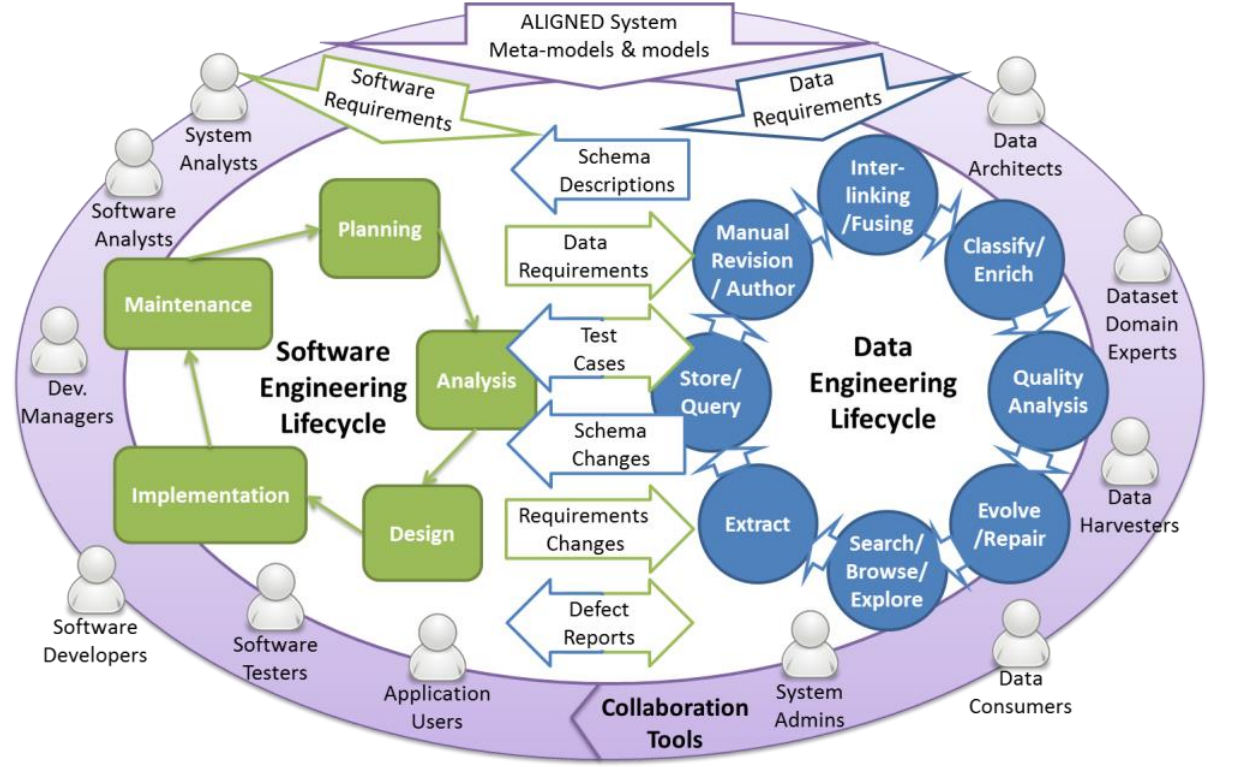
\includegraphics[width=\textwidth]{images/AlignedCircles.png}
  \caption{ALIGNED Software and Data Engineering Processes}
  \label{fig:aligned}
\end{figure}
\todo{add a last sentence?}

\section{Structure}
\label{sec:structure}
This work is a comprehensive introduction to \dataid, with a particular focus on the \core ontology, at the heart of the \ecosystem. It is largely based on four publications:
\begin{enumerate}
\item Martin Brümmer, Ciro Baron, Ivan Ermilov, \underline{Markus Freudenberg}, Dimitris Kontokostas and Sebastian Hellmann  "DataID: Towards Semantically Rich Metadata for
Complex Datasets". In: Proceedings of the 10th International Conference on
Semantic Systems. \cite{dataID2014} - An introduction to the first version of \dataid.
\item Monika Solanki, Bojan Bozic, \underline{Markus Freudenberg}, Dimitris Kontokostas, Christian Dirschl and Rob Brennan "Enabling Combined Software and Data Engineering
at Web-Scale: The ALIGNED Suite of Ontologies". In: The Semantic Web -
ISWC 2016 - 15th International Semantic Web Conference, Kobe, Japan \cite{SolankiBFKDB16} - An overview of the landscape of ontologies developed by the ALIGNED project.
\item \underline{Markus Freudenberg}, Martin Br{\"u}mmer, Jessika R{\"u}cknagel, Robert Ulrich, Thomas Eckart, Dimitris Kontokostas and Sebastian Hellmann "The Metadata Ecosystem of DataID". In: Metadata and Semantics Research: 10th International Conference, MTSR 2016, Göttingen, Germany \cite{Freudenberg2016} - An introduction to the \ecosystem.
\item DataID core Ontology: A W3C member submission of the University of Leipzig, under review by the W3C at the time of writing, authored by Martin Brümmer and me (a preliminary version\footnoteurl{http://vmdbpedia.informatik.uni-leipzig.de/temporary/html/dataid-submission-pre.html}).
\end{enumerate}

After a look at related work (\Cref{chap:relatedwork}) on the subject of dataset metadata, I will present the \ecosystem in Chapter 4, to introduce the guiding principles of this work. Chapter 5 describes the \core ontology in detail, containing a running example of a 
\dbpedia language edition (cf. \Cref{sec:dbpedia}). 
Chapter 6 provides a best practice about publishing data on the Web with \dataid, followed by an application of those practices to an application on how to solve complex metadata challenges with the \ecosystem, by looking at Data Management Plans (\Cref{chap:dmp}).
Chapter 8 provides mappings between \dataid and multiple \cmd profiles of the Component MetaData Infrastructure (\cmdi). \dataid will be evaluated in Chapter 9. A discussion on its development and future work follows in Chapter 10. 
%In a previous version of DataID\cite{dataID2014} we already provided a solution for an accessible, compatible and granular best-practice of dataset descriptions for Linked Open Data (LOD).

%We want to build on this foundation, presenting improvements in regard to Provenance, Licensing and Access. In particular, we want to address the aspects Extensibility and Interoperability of dataset metadata, demonstrating the universal applicability of DataID in any domain or scenario.
%As a proof of concept for its Extensibility we will show how to provide extensive metadata for Data Management Plans (\dmp) of research projects (cf. \Cref{dmps}) by extending the DataID model with properties specific to this scenario.
%The Interoperability with other metadata models is exemplified by the mapping of common \cmdi (CLARIN) profiles to DataID in \Cref{cmdi}.

\chapter{Foundations}
\label{chap:foundations}

\section{Data}
\label{sec:data}
\important{Data} is an almost intangible term. It is highly ambiguous and touches many fields of interest, stretching from philosophy to digital signal processing. Even in the context of Information Science, \important{Data} has multiple possible definitions. Here are some of them:

\begin{quote}
"Data is a symbol set that is quantified and/or qualified." (Prof. Aldo de Albuquerque Barreto, Brazilian Institute for Information in Science
and Technology, Brazil \cite{Zins2007})
\end{quote}

\begin{quote}
"Data are sensory stimuli that we perceive through our senses." (Prof. Shifra Baruchson–Arbib, Bar Ilan University, Israel \cite{Zins2007})
\end{quote}

\begin{quote}
"By data, we mean known facts that can be recorded and that have implicit meaning." (Prof. Shamkant Navathe, College of Computing at the Georgia Institute of Technology, USA \cite{elmasri06db})
\end{quote}

\begin{quote}
"Etymologically, data [...] 
is the plural of datum, a noun formed from the
past participle of the Latin verb dare–to give. Originally,
data were things that were given (accepted as "true"). A data
element, d, is the smallest thing which can be recognised as
a discrete element of that class of things named by a specific
attribute, for a given unit of measure with a given precision
of measurement." (Prof. Charles H. Davis, Indiana University, USA \cite{Zins2007})
\end{quote}

\begin{quote}
"Data are the basic individual items of numeric or other information,
garnered through observation; but in themselves,
without context, they are devoid of information."
(Dr. Quentin L. Burrell, Isle of Man International Business School, Isle of Man \cite{Zins2007})
\end{quote}

Information and \important{Data} seem to be closely linked and are often used interchangeably, yet they are not the same thing:

%Data has become the crude oil of the information age, to the extent where we can no longer speak of ours as an "information society". The call of new, vast, untapped data lakes representing limitless potential value has driven businesses, researchers and governments into an frenzied activities to produce, collect and spy out new data. The "data society" seems to be the appropriate branding of these new surroundings.

%\blockquote[\cite{ventre2016information}]{
%"Data represent the raw material, the resource , which feeds and flows through our systems, the global network of communications between individuals, between machines ans systems. Companies produce data, as do individual citizens, institutions, and the technical systems themselves; data have acquired a market value, a strategic value, so people steal them and resell them [...]."
%}
%Technical and social challenges arising from the ever-increasing flow of Data are plentiful and diverse (as touched on in the introduction of this work). 


\begin{quote}
"Datum is every thing or every unit that could increase the
human knowledge or could allow to enlarge our field of scientific,
theoretical or practical knowledge, and that can be
recorded, on whichever support, or orally handed. Data can
arouse information and knowledge in our mind." (Prof. Maria Teresa Biagetti, University of Rome 1, Italy; based on C. S. Peirce, 1931,
1958 \cite{Zins2007})
\end{quote}

I will take a broader look at the term \important{Data}, delineating it from the concepts of Information and Knowledge.

\subsection{Data, Information, Knowledge}
\label{sec:kids}

\important{Data} is the result of the application of syntactical rules against a set (sequence, string, etc.) of signs or signals, out of which a message between a sender and recipient is constructed \cite{bodendorf2003daten}. Additional schematics might apply, adding structural data. \important{Information} can be gleaned from \important{Data} if one can find meaning in it. The result of this semantic expansion (or interpretation) of \important{Data} can be weighted by its novelty value or exceptionalness in the context of existing \important{Information}, using Shannon's entropy \cite{shannon48}. \important{Data} becomes tokens of perceptions, or more commonly used in Information Science: instances of concepts, capable of changing the understanding of a context for the recipient of the original message. Linking \important{Information} in a context to determine their interrelations and inferring additional \important{Information} under the presumption of an intellectual goal, are the processes (\textit{Pragmatics}) turning \important{Information} into \important{Knowledge}.

\begin{figure}[t]
\centering
  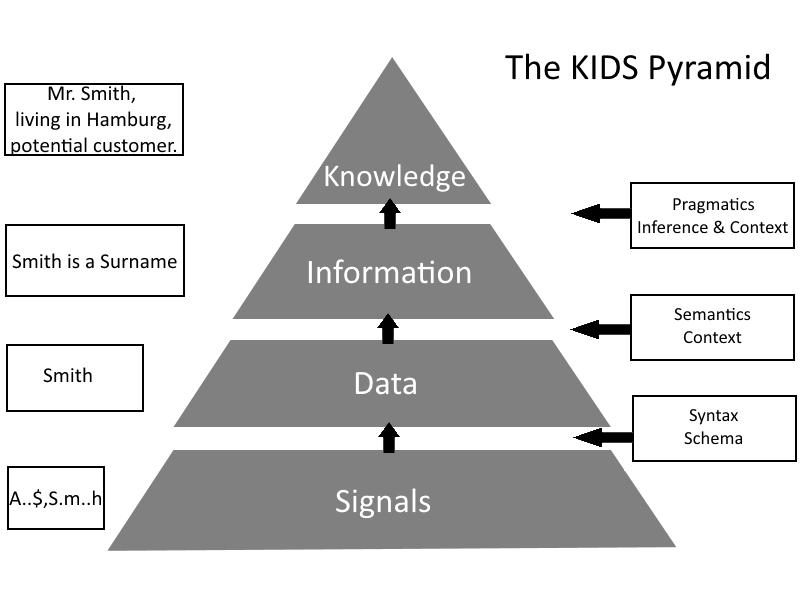
\includegraphics[width=\textwidth]{images/kidsPyramid.png}
  \caption{The KIDS Pyramid \cite{bodendorf2003daten}}
  \label{fig:kids}
\end{figure}

The pyramidal structure depicted (\Cref{fig:kids}) is often crowned by an additional field called "Wisdom" \cite{Rowley2007}. Wisdom could be described as a form of evaluated \important{Knowledge} or understanding, as the pinnacle of human endeavour or enlightenment. But in the era of fake news, pathological mistrust and truthiness\footnoteurl{https://en.wikipedia.org/wiki/Truthiness}, this last step does not seem to follow naturally.

Many authors describe this hierarchy or derivations of it. The following common aspects are presented throughout this literature \cite{Rowley2007}: 

\begin{itemize}
\item the key elements are \important{Data}, \important{Information} and \important{Knowledge},
\item these key elements are virtually always arranged in the same order, some models offer additional stages, such as wisdom, or enlightenment,
\item the higher elements in the hierarchy can be explained in terms of the lower elements by identifying an appropriate transformation process,
\item the implicit challenge is to understand and explain how \important{Data} is transformed into \important{Information} and information is transformed into \important{Knowledge}.
\end{itemize}

\subsection{Digital Data}
\label{sec:digital}
\important{Digital Data} is represented using the binary number system of ones (1) and zeros (0). Typically, these are combined into eight of their kind - named Byte. Bytes are used to identify characters of a given alphabet, which, in turn, provide the building stones for any operation, program or data point (datum).

In general, the term \important{Digital Data} is used to describes a collection of bytes, representing a digital mapping of an analogue counterpart (e.g. sound waves), or characters of an alphabet understood by humans or machines.

\important{Digital Data} is often categorised in structured and unstructured data. Unstructured data does not follow any predefined model and has to be interpreted by the recipient (reader) by its own merit (usually free text). Structured data is strictly adherent to a given data model, facilitating the interpretation of data by machines and humans alike (e.g. Schema Definition Language - XSD \cite{xsd}). 
%Semi structured data allows for unstructured parts in a structured context (e.g. XML [needs link]).

\subsection{Dataset}
\label{sec:dataset}

A \important{Dataset}\footnote{or 'data set', though this spelling seems to be replaced more and more} is a bundle of data points, which have at least one common dimension of distinction. For example, a music album of an artist can be viewed as a \important{Dataset}, where a single song represents a unit of data. Multiple songs are collected in an album with the common feature (among others) - the artist. Most commonly a \important{Dataset} corresponds to a collection of structured (digital) data in a single location (e.g. a database table, XML document etc.).

\important{Datasets} can manifest in different formats (e.g. in different file types). Therefore, the distinction between \important{Dataset} as a container for collecting data points of similar content or structure, and its final manifestation on a file system (database, service endpoint, etc.) is advisable.


\subsection{Metadata}
\label{sec:metadata}

The National Information Standards Organization\footnoteurl{http://www.niso.org/home/} (NISO), a United States non-profit standards organisation, published a paper in 2004, defining \important{Metadata} in a widely adopted manner:

\begin{quote}
"Metadata is structured information
that describes, explains,
locates, or otherwise makes it
easier to retrieve, use, or manage
an information resource. Metadata
is often called data about data or
information about information." \cite{NISO2004}
\end{quote}

\important{Metadata} does not contribute additional content to the original message, but it can ease its transmission, processing and understanding.
The meaning of the term \important{Metadata}, and for what kind of data it applies, is different, depending on context, disciplines and communities.
For example, library catalogue information about a certain book might be understood as \important{Metadata} in regard to the book itself, while in the context of a Library Management System this type of \important{Metadata} is considered data.

Specialised types of \important{Metadata} can be broadly separated into three types \cite{NISO2004}:

\begin{itemize}
\item \important{Descriptive Metadata} describes a resource for purposes such as discovery and identification. It can include elements such as title, abstract, author, and keywords. 
\item \important{Structural Metadata} indicates how compound objects are put together, for example, how pages are ordered to form chapters.
\item \important{Administrative Metadata} provides information to help manage a resource, such as when and how it was created, file type and other technical information, and who can access it. Subsets of administrative \important{Metadata} include:
\begin{itemize}
\item \important{Rights Management Metadata}, which deals with intellectual property rights and licenses.
\item \important{Preservation Metadata}, which contains information needed to archive and preserve a resource.
\end{itemize}
\end{itemize}

A \important{Metadata} record conforms to a given schema since the use of unstructured data to qualify a different data resource is an exercise in futility. Various \important{Metadata} schemata or ontologies are available, often describing similar types of data. The most commonly used \important{Metadata} vocabulary is Dublin Core\footnoteurl{http://dublincore.org/documents/dces/} (DC) by the Dublin Core Metadata Initiative (DCMI):

\begin{quote}
"The original objective of the
Dublin Core was to define a set of
elements that could be used by
authors to describe their own Web
resources. [...] the goal was to define a
few elements and some simple
rules that could be applied by
noncatalogers [sic]." \cite{NISO2004}
\end{quote}

The following example illustrates the use of Dublin Core attributes (e.g. \prop{dc:description}) to describe a publication released as a PDF file:

\begin{lstlisting}[language=ttl, captionpos=b, caption=Dublin Core example, label=lst:dcex,linewidth=\columnwidth,breaklines=true]
dc:title="Metadata Demystified"
dc:creator="Brand, Amy"
dc:creator="Daly, Frank"
dc:creator="Meyers, Barbara"
dc:subject="metadata"
dc:description="Presents an overview of metadata conventions."
dc:publisher="NISO Press"
dc:publisher="The Sheridan Press"
dc:date="2003-07-01"
dc:type="Text"
dc:format="application/pdf"
dc:identifier="http://www.niso.org/standards/resources/metadata.pdf"
dc:language="en"
\end{lstlisting}

All Dublin Core attributes are optional, repeatable (non-functional) and present without order. 
%Controlled vocabularies\footnote{a set of predefined values, controlled by an institution or a body of experts} are recommended to be used in connection with some fields (such as \prop{dc:subject}).
Since its introduction in 1995, the initial list of 15 attributes has been revised and extended, forming the so-called DCMI Metadata Terms\footnoteurl{http://dublincore.org/documents/dcmi-terms/} (DCT). The very general character of this vocabulary provides a useful foundation for more complex schemata reusing DC (e.g. the Data Catalog Vocabulary).

\important{Metadata} can describe any resource in any state or aggregation (single resource, collections, a part of a resource), at any abstraction level of a domain model.
The International Federation of Library Associations and Institutions\footnoteurl{http://www.ifla.org} (IFLA) defined the "Functional Requirements for Bibliographic Records" \cite{IFLA-Functional-1998}, a conceptual model for retrieval and access in online library catalogues and bibliographic databases: \textbf{Item} is an example of a \textbf{Manifestation}, which embodies an \textbf{Expression}, realising a \textbf{Work} of an author.

"For example, a \important{Metadata} record could describe a report, a particular edition of the report, or a specific copy of that edition of the report." \cite{NISO2004}

\important{Metadata} can be embedded in the described digital object, alongside the object (e.g. in the same directory) or stored separately. HTML documents often keep \important{Metadata} in the HTML header or completely emerged in the document (cf. RDFa \cite{McCarronRDFaW3C2015}). While a close coupling between data and \important{Metadata} is useful when updating them together, a separate approach often simplifies the management of large numbers of records.

The advantages of reliable \important{Metadata} for digital objects are manifold. These are the more noteworthy attributions of \important{Metadata}:

\begin{description}
\item [Resource Discovery:] \important{Metadata} is the foremost source of information which aids agents (persons, software, etc.) to discover wanted data.
\item [Organising Electronic Resources:] Entities (e.g. books in a library) are organised in catalogues with the help of their digital \important{Metadata} records.
\item [Interoperability:] The interoperability of two digital resources can be determined by comparing their \important{Metadata} entries, on a syntactical as well as on a semantic level.
\item [Digital Identification:] Digital identifiers (such as URIs \Cref{sec:semweb}) are stored with \important{Metadata} records.
\item [Provenance:] An extensive record on provenance is a key for trustworthiness, detailing facts like source data, responsible agents or origin activities.
\item [Quality:] The quality of a data source can be enhanced significantly by rich \important{Metadata} records.
\item [Reusability:] Increasing discoverability, interoperability, provenance and quality are instrumental requirements for increasing reusability. 
\item [Preservation:] "Metadata is key to ensuring that resources will survive and continue to be accessible into the future." \cite{NISO2004}
\end{description}

In the chain of processes transforming Signals, Data, Information into Knowledge (\Cref{sec:kids}), \important{Metadata} can help with all transformation steps:

\begin{itemize}
\item To provide information about schemata to which a set of structured data adheres or the syntax description needed to understand the signs transmitted.
\item To advance the interpretation of data by providing context information (e.g. geographical or temporal).
\item To point out related (web-) resources to broaden the context of information (e.g. links to similar \important{Datasets} or related website).
\end{itemize}

Based on the observations of \cite{NISO2004}, as well as the concepts common to all domains of \important{Metadata} (discussed in \cite{MetadataPrinciples}), \important{Good Metadata} follows these principles:

\begin{description}
\item[Simplicity] "Key to the simplicity of [a language] is both limited vocabulary and simple structure." \cite{SimplicityComplexity} In the context of \important{Metadata} vocabularies:
A few general metadata terms which are applicable to any domain or use case and are understood by anyone.
\item[Modularity] "It allows designers of metadata schemas to create new assemblies based [...]." \cite{MetadataPrinciples}
on established \important{Metadata} schemas and benefit from observed best practice.
\item[Reusability] "Reuse is the extent to which [an object] can operate effectively for a variety of users in a variety of [...] contexts over time to achieve the same or a different objective from that envisaged by its supplier." \cite{Palmer}
\item[Extensibility] A set of core elements can be extended with further elements to describe the specific data of particular relevance to a community.
\item[Interoperability] "[...] is the ability of multiple systems with different hardware and software platforms, data structures, and interfaces to exchange data with minimal loss of content and functionality." \cite{NISO2004}
\end{description}

In general, the argument can be made that simplicity and modularity are prerequisites for reusability, extensibility and interoperability.

%Metadata for datasets should provide for all of these benefits and reflect the FAIR principles (see next section \ref{sec:fair}). Specifically, dataset metadata should feature:

%\begin{itemize}
%\item machine readable resources (no free text if possible);
%\item well defined abstraction levels (e.g. dataset, dataset catalogue etc.);
%\item a detailed portrayal of internal hierarchies (sub-datsets);
%\item exhaustive descriptions for data access (e.g. access procedures, capacity limitations etc.)
%\item detailed license and rights portrayal
%\item capability for an extensive description of provenance information (involved agents, source datasets etc.)
%\end{itemize}

%These demands on dataset metadata are not particularly unique features, but are of enormous importance to automatically process and evaluate metadata and the described data alike.
\pagebreak
\subsection{The FAIR Data Principles}
\label{sec:fair}

In 2014, a workshop in Leiden, Netherlands, was held, named "Jointly Designing a Data Fairport". A wide group of academics and representatives of companies and other organisations concluded the workshop by drafting a concise set of principles to overcome common obstacles, impeding data discovery and reuse of (scientific) data for humans and machines alike.

\begin{quote}
"[...] humans increasingly rely on computational
agents to undertake discovery and integration tasks on their behalf. This necessitates machines to be capable of autonomously and appropriately acting when faced with the wide range of types, formats, and access-mechanisms/protocols [...]. It also necessitates that the machines keep an exquisite record of provenance such that the data they are collecting can be accurately and adequately cited." \cite{fair2016}
\end{quote}

% According to Wilkonson: "the FAIR Principles put specific emphasis on enhancing the ability of machines to automatically find and use the data, in addition to supporting its reuse by individuals

The \textbf{FAIR} Guiding Principles as drafted by the attendees of this workshop \cite{fair2016}:

\begin{enumerate}
\item[\textbf{F}] \textbf{To be Findable:}
\begin{enumerate}[1]
\item (meta)data are assigned a globally unique and persistent identifier
\item data are described with rich metadata (defined by R1 below)
\item metadata clearly and explicitly include the identifier of the data it describes
\item (meta)data are registered or indexed in a searchable resource
\end{enumerate}
\item[\textbf{A}] \textbf{To be Accessible:}
\begin{enumerate}[1]
\item (meta)data are retrievable by their identifier using a standardized communications protocol
\begin{enumerate}
\item the protocol is open, free, and universally implementable
\item the protocol allows for an authentication and authorization procedure, where necessary
\end{enumerate}
\item metadata are accessible, even when the data are no longer available
\end{enumerate}
\item[\textbf{I}] \textbf{To be Interoperable:}
\begin{enumerate}[1]
\item (meta)data use a formal, accessible, shared, and broadly applicable language for knowledge representation.
\item (meta)data use vocabularies that follow FAIR principles
\item (meta)data include qualified references to other (meta)data
\end{enumerate}
\item[\textbf{R}] \textbf{To be Reusable:}
\begin{enumerate}[1]
\item (meta)data are richly described with a plurality of relevant attributes
\item (meta)data are released with a clear and accessible data usage license
\item (meta)data are associated with detailed provenance
\item (meta)data meet domain-relevant community standards
\end{enumerate}
\end{enumerate}

The basic notion reflected by these principles is, that a minimal set of community-agreed guiding principles would help to access, appropriately integrate, re-use and cite the vast amount of data (generated continuously around the world). Which is especially important for machines, for their lack of an "intuitive sense of 'semantics'" \cite{fair2016}.

Additionally, a scale for reflecting the 'FAIRness' of a repository or its contained data objects was formulated. The different 'levels for FAIRness' are \cite{force11}:

\begin{enumerate}
\item Each Data Object has a PID\footnote{persistent identifier} and intrinsic FAIR metadata (in essence 'static')
\item Each Data Object has 'user defined' (and updated) metadata to give rich provenance in FAIR format of the data, what happened to it, what it has been used for, can be used for etc., which could also be seen as rich FAIR annotations.
\item The Data Elements themselves in the Data Objects are 'technically' also FAIR, but not fully Open Access and not Reusable without restrictions (for instance Patient data or Proprietary data).
\item The metadata as well as the data elements themselves are fully FAIR and completely public, under well defined license. (Non-licensed data considered 'public' by their owner will still be excluded from integration projects by for instance Pharmaceutical companies).
\end{enumerate}

\begin{figure}[!htbp]
\centering
  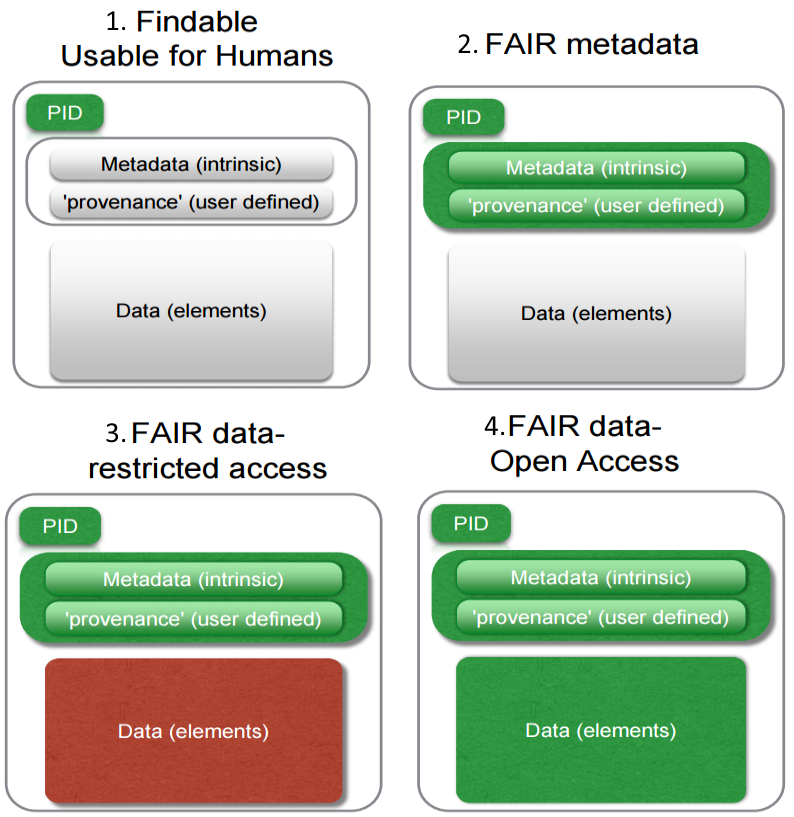
\includegraphics[width=\textwidth]{images/LevelsOfFairData.png}
  \caption{Data Objects with different 'levels of FAIRness' \cite{force11}}
  \label{fig:evalfairlevels}
\end{figure}

\pagebreak
\section{Semantic Web}
\label{sec:semweb}

I presented the common understanding of how data can herald information and knowledge in \Cref{sec:kids}. I refrained from specifying which step or state might be restricted to humans or machines. None of those restrictions would probably be correct. While I don't want to elaborate on the question of: "Can machines have Knowledge?", I do state that machines can glean information from data. To interpret a message and derive meaning is not limited to the human mind. All that is needed is context and an understanding of the concepts and relations constituting a domain (semantics).

In 2001, Tim Berners-Lee, Hendler, and Lassila laid out their expectation of how the World Wide Web will eventually extend to become a Semantic Web \cite{Semweb1}. The simple extension of web resources with structured, well-defined data (or metadata) would give meaning to resources, previously only decipherable by humans. To identify these data resources uniquely by Universal Resource Identifiers (URI) and provide links to other resources, would be the first steps in the direction towards a "web of data" \cite{Semweb1} that can be processed directly by machines.

\begin{quote}
"The Semantic Web is not a separate Web but an extension of the current one, in which information is given well-defined meaning, better enabling
computers and people to work in cooperation." \cite{Semweb1}
\end{quote}

Tim Berners-Lee is the director of the World Wide Web Consortium\footnoteurl{https://w3.org} (W3C), which is responsible for the development of open standards for the World Wide Web, and by extension for the Semantic Web. At its core, the Semantic Web is defined by a collection of standards, which are \textit{Recommendations} by the W3C. "Semantic Web technologies enable people to create data stores on the Web, build vocabularies, and write rules for handling data." \footnoteurl{https://w3.org/standards/semanticweb/}.

\subsection{Resource Description Framework (RDF)}
\label{sec:rdf}

This foundational technology of the Semantic Web and recommendation of the W3C \cite{RDF11} is used to describe any resource, using URIs as identifiers. Resources are defined by a set of characteristics which are expressed as attributes or relations to other resources. Statements in the form of "subject, predicate, object" (named "triples") are used to convey such characteristics. The resource described is uniquely identified by the URI of the subject. The object corresponds to the content or reference of the statement. Literals (strings) are used to serialise content (or values), URIs of resources provide the target of a reference. The predicate is the semantic link between the subject and the object and defines the meaning of this statement.
This simple linguistic construct makes RDF data understandable for humans and machines alike:

\begin{lstlisting}[language=ttl, label=lst:triple,linewidth=\columnwidth,breaklines=true]
<http://dbpedia.org> -> publisher -> "DBpedia Association"
\end{lstlisting}

This triple describes the resource http://dbpedia.org (identified by the URI of the subject). Its object is the literal "DBpedia Association" connected to the subject with the predicate: publisher. Without the predicate, no meaning could be ascribed to the datum "DBpedia Association", as the type of relation between subject and object would be unknown. Thus, the predicate is what lends meaning to a statement.

The same information about the publisher of a website could be expressed differently in RDF data model. Since "DBpedia Association" represents an organisation, it could be introduced and described as an instance of a concept named "Organisation". This instance is capable of providing multiple attributes:

\begin{lstlisting}[language=ttl, label=lst:graph,linewidth=\columnwidth,breaklines=true]
<http://dbpedia.org> -> publisher -> <http://dbpedia.org/DBpediaAssociation>
<http://dbpedia.org/DBpediaAssociation> -> type -> "Organisation"
<http://dbpedia.org/DBpediaAssociation> -> name -> "DBpedia Association"
<http://dbpedia.org/DBpediaAssociation> -> headquarter -> "Leipzig" 
\end{lstlisting}

It is obvious that the instantiation of the objects "Organisation" and "Leipzig" would bear the same benefits. 
By extending this list of statements, describing additional resources and their characteristics, a directed graph is constructed, where nodes are represented by a resource and vertices are relations between resources. A URI can identify a resource without ambiguity (when carefully constructed based on HTTP domain names). This allows for linking of resources without regard to resource locations (datasets, service endpoints, etc.), data restrictions (e.g. licenses) or accessibility, creating, what is called, "Linked Data" (\Cref{sec:ld}).

While labels like "publisher" have meaning for humans, they are ambiguous and could be misinterpreted. 
Especially machines cannot resolve this ambiguity and could not infer meaning from such statements. 
To address this issue, predicates are also identified by URIs that can be looked up for further information. The example below displays a valid RDF syntax called N-Triples.

\begin{lstlisting}[language=ttl, label=lst:graph,linewidth=\columnwidth,breaklines=true]
<http://dbpedia.org> <http://purl.org/dc/terms/publisher> <http://dbpedia.org/DBpediaAssociation>.
<http://dbpedia.org/DBpediaAssociation> <http://purl.org/dc/terms/name> "DBpedia Association".
\end{lstlisting}

Predicates are called properties in the RDF data model.
Sets of properties can be defined and documented by institutions (such as the DCMI - cf. \Cref{sec:metadata}), which , in turn, can be used by others, increasing interoperability and reusability. These sets of properties together with associated concepts and annotations are called ontologies or vocabularies.


\subsection{Web Ontology Language (OWL)}
\label{sec:owl}

The Web Ontology Language is a W3C standard \cite{OWL2} based on the RDF data model, which could be summarised as an ontology for defining ontologies. 
According to Gruber,
\begin{quote}
"An ontology is an explicit specification of a conceptualization." \cite{Gruber}
\end{quote}

I delineate an ontology as a set of concepts, properties and logical axioms, with which to model a domain of knowledge or discourse. This conceptualization of a given domain or idea allows for a schema-bound representation of data with RDF as well as its automatic interpretation by machines.

Concepts are classes under which all objects of a domain can be classified, dividing up the domain in abstract objects. Properties provide meaning for the links to instances of concepts or literal objects (values), which, in turn, lends meaning to the concepts themselves. Additionally, subclass relations and restrictions on properties (e.g. domain and range definitions) help to specify more complex relations of a domain. This semantic layer between the domain knowledge on one side and its representation in RDF on the other is free of restrictions imposed by underlying technologies, distinguishing it from other data models (e.g. database schemata). A wide range of ontologies is available for any domain. Upper ontologies are general use vocabularies (such as Dublin Core \Cref{sec:metadata}) which can be reused together with other ontologies. High reusability is a desirable feature of any ontology.
OWL is based (with some restrictions) on the RDF Schema (RDFS \cite{RDFS11}), which provides basic elements for the description of ontologies (allowing for class hierarchies and basic relations).
Multiple profiles are available \cite{OWLPROFILES}, introducing different logical regimes to OWL, such as Description Logic (OWL-DL) or based on Rule Languages (OWL2-RL). Profiles allow for reasoning over RDF data, adhering to ontologies under such regimes. 

Description Logic is a fragment of first-order predicate logic \cite{Barwise1977} and a formalism for representing knowledge under an \textit{Open World Assumption}. OWL is heavily influenced by Description Logic (projects like DAML+OIL \cite{HPMW07}) to achieve a beneficial trade-off between language expressiveness and computational complexity of reasoning.


\subsection{Linked Data}
\label{sec:ld}
Linked Data is the idea of how data is freed from islands of unconnected data, so it can be reused all over the World Wide Web referencing simply its URIs. Links between data objects from different sources are not bound to restrictions, authorisation procedures, licensing or any technical obstacles, they simply state that: 'There is a data object (published in a well-defined manner - e.g. RDF) which is related and it is identifiable on the Web with this URI.' Machines and humans can follow up these links and explore the 'Web of Data', expanding the contextual information.

\begin{quote}
"Technically, Linked Data refers to data published on the Web in such a way that it is
machine-readable, its meaning is explicitly defined, it is linked to other external data sets,
and can, in turn, be linked to from external data sets." \cite{bizer_linked_2009}
\end{quote}

Additionally, a set of best practices were contrived by Tim Berners-Lee to identify the necessary steps needed to publish and link structured data on the Web, since "a surprising amount of data isn't linked in 2006, because of problems with one or more of the steps" \cite{5starData}.

\begin{enumerate}
\item Use URIs as names for things.
\item Use HTTP URIs so that people can look up those names.
\item When someone looks up a URI, provide useful information, using the standards (RDF, SPARQL).
\item Include links to other URIs, so that they can discover more things.
\end{enumerate}

Linked Data extends the demands of RDF as a data model by specifying HTTP as the access
layer and requiring the openness of the resource to be regarded of high quality. 
The result is a 'Web of Data', a machine-readable, semantic network of structured data, 
opposed to the HTML-based web of documents (from humans, for humans).

\chapter{Related Work}
\label{chap:relatedwork}

\section{Dataset vocabularies}
\label{sec:dv}
This section is dedicated to dataset metadata vocabularies and application profiles, to compare them and list their (dis-) advantages.

Based on the attributes of 'Good Metadata' (cf. \Cref{sec:metadata}), the FAIR Data Principles (\Cref{sec:fair}) and my own list of principle goals of dataset metadata (\Cref{sec:objectives}), I contrived the following list of aspects, against which I want to evaluate each vocabulary.

\begin{enumerate}[A]
\item \textbf{The vocabulary encourages the use of richly described and machine-readable resources.} 
Concepts are defined as exhaustive as necessary to describe all relevant aspects, avoiding free text properties in general. For example, replacing a literal with a well-structured instance of \prop{foaf:Agent}. 
\item \textbf{The vocabulary assigns globally unique URIs to metadata resources.} Demanding URIs as identifiers, independent of the chosen data representation (even for non-RDF or XML metadata).
\item \textbf{The vocabulary can describe data access and access restrictions, consumable for humans and machines alike.} Sufficient effort has been made to describe the technical aspects of data access and possible restrictions to it (e.g. API authorisation methods), considering all possible formats of a dataset (files, APIs, etc.).
\item \textbf{The vocabulary can portray provenance information extensively.} Dataset provenance can be described extensively, including other datasets (e.g. sources), activities (e.g. data generation activities) and agents (e.g. publisher) as well as inter-relational properties between these concepts.
\item \textbf{The vocabulary provides for detailed descriptions of rights and licenses.} Machine readable licenses are of utmost importance.
\item \textbf{The vocabulary provides properties to cite identifiers of the data described.} The possibility to reference the data described directly (by identifier) in the metadata is available.
\item \textbf{The vocabulary provides for qualified references between resources.} Relations between instances of dataset metadata can be qualified by roles (specifying the type of relations), time and other restrictions.
\item \textbf{The vocabulary is easy to extend, to fit any given use case.} The vocabulary can extend easily. No unnecessary restrictions impeding Extensibility, like restrictive cardinalities, are in place.
\item \textbf{The vocabulary is unambiguous and easy to map to other metadata vocabularies.} The vocabulary is general enough to be able to interoperate with other metadata formats. Properties are defined clearly without semantic overlap to others (so users know which properties to use).
\item \textbf{The vocabulary offers additional properties to aid dissemination and discovery.} Properties are in place to provide keywords, genres, taxonomies and general statements explaining the intention, use or gain of a dataset.
\end{enumerate}

I will assign one of the following ratings to every item: \textbf{(2)} The requirement is supported in full. \textbf{(1)} The requirement is partially met. \textbf{(0)} The vocabulary does not support this requirement. 
While this list is helpful for evaluation and comparison purposes, the quality of a dataset vocabulary is also dependent on the intended domain of use and other factors, which I will mention as well. A summary of these findings is available as part of the evaluation (cf. \Cref{sec:evalvocabularies}).

\subsection{The Data Catalog Vocabulary (DCAT)}
\label{sec:dcat}
In \cite{MaaliCP10} the authors introduce a standardised interchange format for machine-readable representations of government data catalogues. The Data Catalog Vocabulary (\dcat) is a W3C recommendation \cite{ddcat} and serves as a foundation for many available dataset vocabularies and application profiles.
Vocabulary terms for \dcat are inferred from the survey on seven data catalogues from Europe, US, New Zealand and Australia.

\begin{quote}
"By using \dcat to describe datasets in data catalogs, publishers increase discoverability and enable applications easily to consume metadata from multiple catalogs. It further enables decentralized publishing of catalogs and facilitates federated dataset search across sites." \cite{ddcat}
\end{quote}

\dcat defines three levels of abstraction, based on the following distinctions: A dataset describes a "collection of data, published or curated by a single agent, and available for access or download in one or more formats" \cite{ddcat}, and represents the commonalities and varieties of the data held within (the 'idea' or intellectual content of that dataset). A Dataset is part of a data catalogue, representing multiple datasets (e.g. of an organisation). Datasets manifest themselves (are available) in different forms (such as files, service endpoints, feeds, etc.), expressed with the class \prop{dcat:Distribution}. A dataset might be available for download at two different locations on the Web and available to be queried through an API endpoint. This scenario is describable by using three different \prop{dcat:Distribution} instances.

\begin{figure}[!htbp]
\centering
  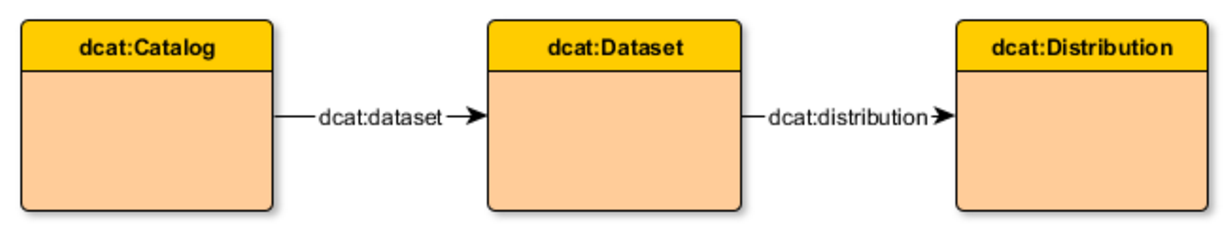
\includegraphics[width=\textwidth]{images/DcatIdea.png}
  \caption{The basic idea of \dcat}
  \label{fig:dcat}
\end{figure}

This basic idea of differentiating between catalogue, dataset and distribution, has prevailed throughout the metadata domain for digital resources (not only datasets), and has become a quasi-requirement for metadata representations of web resources\footnoteurl{https://www.w3.org/TR/dwbp/#context}. In fact, the general approach the authors of \dcat took, makes it possible to describe any digital object. This is a highly desirable feature, supporting Extensibility and Interoperability of the vocabulary.

A downside to this approach is the possible unspecificity of resources, especially regarding machine-readability, where uncertainty about formats is problematic. The full list of possible issues with exclusive \dcat solutions:

\textbf{Insufficient provenance information:}
\begin{itemize}
\item \dcat expresses provenance in a limited way using a few basic properties such as
\prop{dct:source} or \prop{dct:creator}, which can not be further qualified.
\item No possibility to specify activities involved in the creation of datasets.
\item There is no support or incentive to describe source datasets, related publications or conversion activities of transformations responsible for the dataset. This lack is crucial, especially in a scientific context, as it omits the processes necessary to replicate a specific dataset.
\item Insufficient portrayal of context information (e.g. licenses, geography, etc.)
\end{itemize}

\textbf{Missing relations between Datasets:}
\begin{itemize}
\item in general: Referencing related datasets is only possible on a very generic scale (e.g. \prop{dct:relation}).
\item hierarchical: No inherent portrayal of dataset hierarchies is possible.
\item evolutionary: No versioning pointers between dataset representations.
\end{itemize}

\textbf{Relations to agents are too cursory:}
\begin{itemize}
\item A very restricted number of properties pointing out agents, without any further qualification (e.g. \prop{dct:publisher}, \prop{dcat:contactPoint}), other related entities, like software, projects, funding, etc., are neglected altogether.
\item No agent role concept to define new relations.
\end{itemize}

\textbf{Technical description of distributions is lacking, restricting the accessibility of the data:}
\begin{itemize}
\item Only superficial attributes for describing the technical characteristics of a distribution are available (e.g. \prop{dcat:downloadURL}).
\item No access information are available, such as access restrictions or service description, needed to describe service endpoints.
\item No specificity when describing serialisation or media type of a distribution (e.g. file format).
\end{itemize}

\textbf{The general lack of specificity, inviting non-machine-readable expressions of resources:}
\begin{itemize}
\item Insufficient specificity of property ranges (e.g.: \prop{dct:license}, \prop{dct:temporal}, \prop{dct:spatial}, \prop{dct:language}, \prop{dcat:mediaType}), thereby neglecting exactness of relevant metadata resources, such as licenses.
\item A lack of referential and functional integrity due to missing role-based qualifications of properties (such as \prop{dct:maintainer}) \cite{jefferyCerifW3C2016}.
\end{itemize}

While this seems to be an extensive list of shortcomings, most of the points listed above are due to the general approach of \dcat. The list merely indicates that portraying dataset metadata with \dcat alone, might not be sufficient for most domains and use cases.

In turn, extending \dcat as upper ontology provides a sufficient basis for any metadata descriptions, without regard to a domain or use case. Adopting not only its basic ideas but the aspects of easy Extensibility and Interoperability, should prove beneficial. Addressing the issues with Provenance, Licensing and Access as well as domain-specific demands for metadata is the central task I set out to complete.

\begin{table}[!htbp]
    \centering
    \begin{tabular}{|l|l|l|l|l|l|l|l|l|l|l|l|}
        \hline
        Requirement & A & B & C & D & E & F & G & H & I & J & Sum \\
        \hline
        Evaluation of \dcat & 1 & 2 & 1 & 0 & 0 & 1 & 0 & 2 & 2 & 1 & 10 \\
        \hline
    \end{tabular}
    \label{tab:evaldcat}
\end{table}

\subsection{Vocabulary of Interlinked Datasets (VoID)}
\label{sec:void}

The Vocabulary of Interlinked Datasets (\void) \cite{Alexander09describinglinked} is widely accepted and used within the Semantic Web community, for instance in projects such as OpenLink Virtuoso\footnoteurl{http://virtuoso.openlinksw.com/} , LODStats\footnoteurl{http://stats.lod2.eu/} , World Bank\footnoteurl{http://worldbank.270a.info/} and others. \void can be used to express general metadata, statistical metadata, structural metadata and links between Linked Data datasets. Tools to create \void metadata are described in \cite{DBLP:BohmLN11} where authors also present techniques of reduction to create descriptions for Web-scale datasets. In the same paper, the importance of \void is well established but there is still a lack of important metadata which is not described, for example for, Licensing and Provenance. For simple datasets, \void performs well, which is supported by the vocabularies wide acceptance amongst many applications in research and industry.
However, in a case of complex datasets \void is not expressive enough. In particular, the access metadata property \prop{void:dataDump}, which points to the data files of the particular dataset, is questionable. This property should link directly to dump files as described in W3C Interest Group Note: Describing Linked Datasets with the \void Vocabulary\footnoteurl{http://www.w3.org/TR/void/}. Thus, additional semantic information about the data files and the structure of the dataset can not be expressed using \void. This lack of a distribution concept is depriving the vocabulary of an important level of abstraction. Nevertheless, this ontology is useful especially for Linked Data datasets, offering many useful statistical properties (such as \prop{void:triples}) and the very handy concept of \prop{void:LinkSet} describing the particular relation between datasets, where one holds links to instances of the other.

\begin{table}[!htbp]
    \centering
    \begin{tabular}{|l|l|l|l|l|l|l|l|l|l|l|l|}
        \hline
        Requirement & A & B & C & D & E & F & G & H & I & J & Sum \\
        \hline
        Evaluation of \void & 1 & 2 & 0 & 0 & 0 & 0 & 1 & 1 & 2 & 1 & 8 \\
        \hline
    \end{tabular}
    \label{tab:evalvoid}
\end{table}

\subsection{Comprehensive Knowledge Archive Network (CKAN)}
\label{sec:ckan}

Metadata models vary, and most of them do not offer enough granularity to describe complex datasets sufficiently in a semantically rich way. 
For example, \ckan{}\footnoteurl{http://ckan.org/} (Comprehensive Knowledge Archive Network), a data management system used widely in (open) data portals (such as datahub.io\footnoteurl{http://datahub.io/}) to provide web representations for datasets, operates on a JSON-based schema\footnoteurl{https://github.com/KSP-CKAN/CKAN/blob/master/CKAN.schema} developed by the Open Knowledge Foundation\footnoteurl{https://okfn.org}.
\ckan allows simple access to a whole range of functions related to the management of datasets (such as search and faceting of data-sources) accessible via a REST interface.
Its metadata schema has some similarities with \dcat: Datasets are collected under organisation objects, which are used as s primitive stand in for catalogues. Datasets have 'Resources' which assume a similar role as a distribution in the \dcat vocabulary. 

Alas, there is no clear definition of the resource-object within \ckan documentation, nor are there any noteworthy restrictions. This has led to a medley of different use cases for this concept, where it assumes the role of a \prop{dcat:Distribution} in one dataset (containing all data of the dataset) and providing different slices of the data in another example \cite{neum-etal-2016w3c}. Furthermore, the extensive use of key-value pairs for additional data led to a sheer host of (semi-) structured data, with only marginal agreement on key names between different Data Portals \cite{neum-etal-2016w3c} adding to the general unclarity of this metadata format, complicating the mapping to other vocabularies.

This data model is semantically poor and inadequate for most applications consuming data automatically. I strongly discourage any organisation from adopting the \ckan format for their dataset metadata. Since it is used so frequently in data portals, I feel obliged to point out that there are mapping tools for most vocabularies to \ckan (as I provided for DataID in \cite{dataID2014}).

\begin{table}[!htbp]
    \centering
    \begin{tabular}{|l|l|l|l|l|l|l|l|l|l|l|l|}
        \hline
        Requirement & A & B & C & D & E & F & G & H & I & J & Sum \\
        \hline
        Evaluation of \ckan & 0 & 2 & 0 & 0 & 0 & 0 & 0 & 1 & 1 & 0 & 4 \\
        \hline
    \end{tabular}
    \label{tab:evalckan}
\end{table}


\subsection{Metashare}
\label{sec:metashare}
The \metashare ontology\cite{mccrae_2015_OWLmetashare} is the offspring of a prior, XSD-based \cite{xsd} "metadata schema that allows aspects of [language resources] accounting for their whole lifecycle from their production to their usage to be described"\cite{mccrae_2015_OWLmetashare}.
\metashare differentiates between language resources (basically datasets with a language related purpose - text, audio etc.), technologies (e.g., tools, services) used for their processing and additional entities like reference documents, agents, projects or licenses. This allows for the portrayal of provenance in the domain of Natural Language Processing.
Also, it offers an exemplary way of describing licenses and terms of reuse\footnoteurl{http://www.cosasbuenas.es/static/ms-rights/}. However, \metashare is highly specialised for language resources, thus lacking generality and extensibility for other use cases. While not implementing the \dcat vocabulary, \metashare does provide an almost complete mapping to \dcat. Mappings to other ontologies might prove difficult, due to the large size of the vocabulary and the often employed (and ample) controlled vocabularies. The related \metashare XSD schema has been implemented in the \metashare web portal\footnoteurl{http://www.meta-share.org}, providing many NLP related datasets for download.

\begin{table}[!htbp]
    \centering
    \begin{tabular}{|l|l|l|l|l|l|l|l|l|l|l|l|}
        \hline
        Requirement & A & B & C & D & E & F & G & H & I & J & Sum \\
        \hline
        Evaluation of \metashare & 2 & 2 & 1 & 1 & 2 & 0 & 0 & 0 & 1 & 1 & 10 \\
        \hline
    \end{tabular}
    \label{tab:evalmetashare}
\end{table}

\subsection{Asset Description Metadata Schema (ADMS)}
\label{sec:adms}
The Asset Description Metadata Schema\footnoteurl{https://www.w3.org/TR/vocab-adms/} (\adms) is a profile of \dcat, which is specialised to describe "Semantic Assets".
Assets (as subclass of \prop{dcat:Dataset}) are highly reusable metadata (e.g. code lists, XML schemata, taxonomies, vocabularies, etc.) expressing the intellectual content of the data, which is represented (in most cases) in relatively small files. 

\adms adopts the \dcat structure and provides a well-defined way of versioning between entities. Its specialised nature makes it unsuited for a broader approach of portraying datasets (as intended by the authors), but it can still contribute useful properties to \dcat based vocabularies (e.g. \Cref{sec:dcatap}). Since \adms does not impose any restrictions, it can be extended to \dcat without any consequences for \dcat based metadata documents. The evaluation below therefore does not differ from \dcat.

\begin{table}[!htbp]
    \centering
    \begin{tabular}{|l|l|l|l|l|l|l|l|l|l|l|l|}
        \hline
        Requirement & A & B & C & D & E & F & G & H & I & J & Sum \\
        \hline
        Evaluation of \adms & 1 & 2 & 1 & 0 & 0 & 1 & 0 & 2 & 2 & 1 & 10 \\
        \hline
    \end{tabular}
    \label{tab:evaladms}
\end{table}

\subsection{DCAT Application Profile for data portals in Europe (DCAT-AP)}
\label{sec:dcatap}

The DCAT Application Profile for data portals in Europe\footnoteurl{https://joinup.ec.europa.eu/asset/dcat_application_profile/home} (\dcatap) is a specification based on \dcat (extended with \adms properties) for describing public sector datasets in Europe. It was developed by a working group under the auspices of the European Commission. Its basic use case is "to enable cross-data portal search for datasets and to make public sector data better searchable across borders and sectors" \cite{dcatap11}. This can be achieved by the exchange of descriptions of datasets among data portals.

Traits of the resulting profile\footnoteurl{https://joinup.ec.europa.eu/catalogue/distribution/dcat-ap-version-11} (version 1.1) released in October 2015 \cite{dekkersDcatApW3C2016}:

\begin{itemize}
\item It proposes mandatory, recommended or optional classes and properties to be used for a particular
application;
\item It identifies requirements to control vocabularies for this application;
\item It gathers other elements to be considered as priorities or requirements for an application such as
conformance statement, agent roles or cardinalities.
\end{itemize}

\dcatap has been endorsed by the Standards Committee of ISA2\footnoteurl{https://ec.europa.eu/isa/isa2/index_en.htm} in January of 2016\footnoteurl{https://joinup.ec.europa.eu/community/semic/news/dcat-ap-v11-endorsed-isa-committee} for the use in data portals. Further, it has been implemented by over 15 open data portals in the European Union, including the European Data Portal\footnoteurl{https://www.europeandataportal.eu/}. 

In general, while some recommendations are in place (e.g. using \odrl license documents - \Cref{sec:odrl}), \dcatap can not propose concrete improvements in extending \dcat to advance Provenance, Licensing or Access. As remarked in section 7 of its specification\footnoteurl{https://joinup.ec.europa.eu/catalogue/distribution/dcat-ap-version-11}, the representation of different agent roles is lacking in the current version of \dcatap. In my opinion, the second solution proposed within, using \prov (Provenance Ontology - see \Cref{sec:prov}), is the most comprehensive way of resolving this issue. Due to some cardinality restrictions (e.g. those on \prop{dcat:accessURL}) and its specialisation for data portals, extending \dcatap to serve more elaborate purposes, can pose challenges. 

\begin{table}[!htbp]
    \centering
    \begin{tabular}{|l|l|l|l|l|l|l|l|l|l|l|l|}
        \hline
        Requirement & A & B & C & D & E & F & G & H & I & J & Sum \\
        \hline
        Evaluation of \dcatap & 1 & 2 & 1 & 0 & 0 & 1 & 0 & 1 & 2 & 1 & 9 \\
        \hline
    \end{tabular}
    \label{tab:evaldcatap}
\end{table}

\subsection{The HCLS Community Profile}
\label{sec:hcls}
The W3C interest group Semantic Web for Health Care and Life Sciences (HCLS)  represents many stakeholders of the Life Sciences, seeking to "develop, advocate for, and support the use of Semantic Web technologies across health care, life sciences, clinical research and translational medicine" \cite{hclsig}. 

Their community profile (an ongoing effort by this W3C interest group\footnoteurl{https://www.w3.org/blog/hcls/}), extends \dcat with versioning and detailed summary statistics, through a three-component model. This model introduces an additional abstraction level between dataset and distribution, the so-called 'Version Level Description', which contains version specific properties (e.g. \prop{dct:isVersionOf}). The profile is structured in multiple modules, dealing with different levels of specificity \cite{HCLSCP2016}:

\begin{description}
\item[Core Metadata] captures generic metadata about the dataset, e.g., its title, description, and publisher.

\item[Identifiers] describe the patterns used for identifiers within the dataset and the URI namespaces for RDF datasets.

\item[Provenance and Change] describe the version of the dataset and its relationship with other versions of the same dataset and related datasets, e.g., an external dataset that is used as a source of information.

\item[Availability/Distributions] provides details of the distribution files, including their formats, in which the dataset is made available for reuse.

\item[Statistics] used to summarise the content of the dataset.
\end{description}

The HCLS profile reuses 18 vocabularies with 61 properties \cite{HCLSCP2016}, covering many goals of my evaluation. The chosen approach of this profile is sound and achieves qualitatively good metadata, with an emphasis on FAIR Data principles.

One problem is the large number of reused vocabularies with overlapping purposes, which cause difficulties when mapping to other vocabularies. Its cardinality restrictions can pose problems when extending the profile to use cases, especially outside the health care domain. Although efforts were made to cover provenance in general, problems like qualifying otherwise static relations to agents or datasets can not be solved by the incorporated vocabularies. The approach to portraying licenses does not improve \dcat.

A specific problem is the use of the property \prop{dcat:accessURL}, which, according to the profile, could be used on the dataset abstraction level ('Summary Level Description'). This clearly violates the specification of \dcat. In general the border between \prop{dcat:Dataset} and \prop{dcat:Distribution} has to be defined more carefully when adding an additional layer in between.

\begin{table}[!htbp]
    \centering
    \begin{tabular}{|l|l|l|l|l|l|l|l|l|l|l|l|}
        \hline
        Requirement & A & B & C & D & E & F & G & H & I & J & Sum \\
        \hline
        Evaluation of HCLS Profile & 2 & 2 & 2 & 1 & 0 & 1 & 0 & 2 & 1 & 1 & 12 \\
        \hline
    \end{tabular}
    \label{tab:evaldcatap}
\end{table}

\subsection{CERIF}
\label{sec:cerif}
The metadata format \cerif\footnoteurl{http://www.eurocris.org/cerif/main-features-cerif} (Common European Research Information Format) is a metadata development, which began in the early 1990s. The shortcomings of its first approach were addressed by CERIF2000, which became an EU recommendation for its member states for research data. Since 2002 \cerif is further developed by the Current Research Information Systems organisation\footnoteurl{http://www.eurocris.org}.

\cerif provides generalised base concepts and relations between them, based on an entity-relationship approach \cite{CerifJefferyA10}. Relations (or 'linking entities') are qualified with roles, temporal and spatial statements, supplemented with provenance and versioning information.
In contrast to Dublin Core based metadata standards (i.e. \dcat), \cerif was developed with a particular focus on referential and functional integrity of resources, avoiding ambiguity in interpretation \cite{jefferyCerifW3C2016}. 
\cerif provides much more than just metadata for datasets, it addresses metadata needs for the whole science community, describing projects, funding, facilities, organisations and other.

This paper lines out the main characteristics of \cerif metadata \cite{jefferyCerifW3C2016}:,
\begin{itemize}
\item it separates base entities from relationships between them and thus represents the more
flexible fully-connected graph rather than a hierarchy;
\item it has generalised base entities with instances specialised by role (e.g. <person> rather
than <author>), in the linking entities;
\item it handles multilinguality by design and temporal information (so representing versions)
to the appropriate attribute treated as an entity (example <title> linked to <publication>);
\item temporal information is in the link entities not the base entities (e.g. employment between
two dates is in the linking relation between <person> and <organisation> and not an attribute of either
of the base entities);
\item the temporal information in linking entities provides provenance and versioning recording (e.g.
versions of datasets and – in the associated role attribute – the method of update or change);
\item \cerif separates the semantics into a special 'layer' which is referenced from \cerif instances. The
semantic layer includes permissible values for roles in any linking entity and controlled
values of attributes in base entities (e.g. ISO country codes). Thus semantic terms are stored once and
referenced many times (preserving integrity). 
\end{itemize}

\cerif offers a comprehensive approach to solving a host of metadata demands in a sophisticated manner. 
The chosen abstraction levels (layers) are appropriate, and the adherence to an entity-relationship approach is arguably a working solution for qualifying relations. The main problem with \cerif is the complexity of its ontology\footnoteurl{http://eurocris.org/ontologies/cerif/1.3/} \footnoteurl{http://eurocris.org/ontologies/semcerif/1.3/} together with the unique approach to metadata (unlike the \dcat based understanding of metadata). The imposes hurdles when studying, mapping and extending this ontology. 
%Also, while it can be used in generic way, \cerif has some very specific properties for research related purposes (e.g. \prop{cerif:linksToFunding}), adding to problems with extending and mapping. 
Furthermore, the ontology proves to be not specific enough when dealing with information on Access and Licensing.

\begin{table}[!htbp]
    \centering
    \begin{tabular}{|l|l|l|l|l|l|l|l|l|l|l|l|}
        \hline
        Requirement & A & B & C & D & E & F & G & H & I & J & Sum \\
        \hline
        Evaluation of \cerif & 2 & 2 & 1 & 1 & 0 & 2 & 2 & 2 & 2 & 1 & 15 \\
        \hline
    \end{tabular}
    \label{tab:evaldcatap}
\end{table}

\subsection{Component MetaData Infrastructure (CMDI)}
\label{sec:cmdi}

The Component MetaData Infrastructure is a component-based framework for the creation and utilisation of metadata schemata\cite{BROEDER10.163}. It allows the distributed development of metadata components (defined as sets of related elements) and their combination to profiles in any level of detail, forming the basis for the creation of resource-specific XML Schemata and around one million publicly available metadata files. \cmdi is a flexible metadata framework, which can be applied to resources from any scientific field of interest. It is especially relevant in the context of the European research infrastructure CLARIN\cite{Hinrichs2014} where it is used to describe resources with a focus on the humanities and social sciences.

The very flexible and open approach of the \cmdi which allows for its wide applicability, may lead in parts to problems regarding consistency and Interoperability.
Despite being rich in descriptive metadata, some \cmd profiles lack consistent information of the kind stated in \Cref{sec:dmprequ}. This includes the explicit specification of involved persons, descriptions of authoritative structures as well as technical details and actual download locations.

The highly modularised nature of this vocabulary makes it hard to attach a single evaluation to it. However, considering the onesided distribution of relevant \cmd profiles to actual metadata instances (cf. \Cref{sec:mapcmdi}), we can base this evaluation on the most probable profiles.

\begin{table}[!htbp]
    \centering
    \begin{tabular}{|l|l|l|l|l|l|l|l|l|l|l|l|}
        \hline
        Requirement & A & B & C & D & E & F & G & H & I & J & Sum \\
        \hline
        Evaluation of \cmdi & 1 & 2 & 0 & 0 & 1 & 2 & 0 & 2 & 0 & 1 & 9 \\
        \hline
    \end{tabular}
    \label{tab:evaldcatap}
\end{table}

\subsection{DataID version 1.0.0}
\label{sec:dataid100}

The common shortcomings of dataset vocabularies revealed in this section were also afflicting the previous version (1.0.0) of the \dataid ontology \cite{dataID2014}. Rooted in the Linked Data world, it neglected important information or provided properties (e.g. \prop{dataid:graphName}) which are orphans outside this domain. 

While it already imported the important Provenance Ontology (\prov  - \Cref{sec:prov}), to cover the general issues with Provenance, it was lacking regarding the specificity of Access and Licensing. The narrow definition of datasets (i.e. restricted to Linked Data datasets) was inadequate for use cases outside this domain and so inhibited Extensibility.

\begin{table}[!htbp]
    \centering
    \begin{tabular}{|l|l|l|l|l|l|l|l|l|l|l|l|}
        \hline
        Requirement & A & B & C & D & E & F & G & H & I & J & Sum \\
        \hline
        Evaluation of DataID 1.0.0 & 1 & 2 & 1 & 1 & 2 & 1 & 2 & 1 & 2 & 1 & 14 \\
        \hline
    \end{tabular}
    \label{tab:evaldataid100}
\end{table}

\pagebreak
\section{Secondary Literature}
\label{sec:auxiliary}

This section proffers a collection of associated literature, not directly touching on the subject of dataset metadata. Many subjects, such as the representation of licenses and data quality, are relevant for providing metadata of datasets.

\subsection{The Provenance Ontology (PROV-O)}
\label{sec:prov}

\begin{quote}
"Provenance is defined as a record that describes the people, institutions, entities, and activities involved in producing, influencing, or delivering a piece of data or a thing. In particular, the provenance of information is crucial in deciding whether the information is to be trusted, how it should be integrated with other diverse information sources, and how to give credit to its originators when reusing it. In an open and inclusive environment such as the Web, where users find information that is often contradictory or questionable, provenance can help those users to make trust judgements." \cite{MoreauProvDM2013}
\end{quote}


The Provenance Ontology\cite{prov} (\prov) is a widely adopted W3C recommended standard and serves as a lightweight way to express the provenance and interactions between activities, agents and entities (e.g. datasets). 

\begin{figure}[!htbp]
\centering
  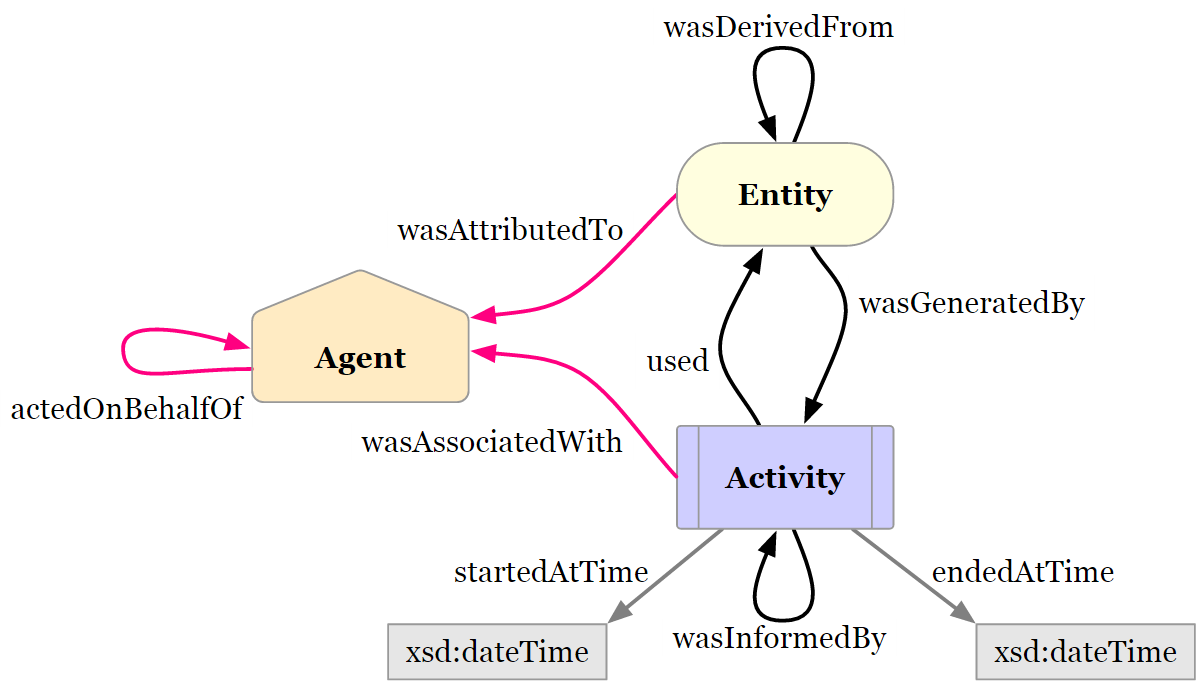
\includegraphics[width=\textwidth]{images/ProvLinchpin.png}
  \caption{Linchpin of the Provenance Ontology: Entities, Agents, Activities \cite{prov}}
  \label{fig:prov}
\end{figure}

%Provenance information is needed in any given scenario. 
In the context of datasets, provenance information on the activities which helped to create a dataset, which agents were involved in these processes and who to contact about it as well as source datasets or other entities involved are of interest, especially when trying to determine the trustworthiness of data. This ontology is "[...] the foundation to implement provenance applications in different domains that can represent, exchange, and integrate provenance information generated in different systems and under different contexts." \cite{prov}

Each of the relations depicted (\Cref{fig:prov}) have suitable qualification classes (e.g. \prop{prov:Association}), so that a property (\prop{prov:wasAssociatedWith}) can be inferred from the qualified property path  (\prop{prov:qualifiedAssociation}/\prop{prov:agent}). Qualification classes provide qualification via properties such as \prop{prov:role}. 

In this example (from the official specification of \prov \cite{prov}), an association provides an additional description about the \prop{:illustrationActivity} that an agent named 'Derek' influenced:

\begin{lstlisting}[language=ttl, captionpos=b, label=lst:dcex,linewidth=\columnwidth,breaklines=true]
@prefix prov: 			<http://www.w3.org/ns/prov#> .
@prefix :     			<http://example.org#> .

:illustrationActivity
   a prov:Activity;                  ## this illustration activity was 
   prov:wasAssociatedWith :derek;    ##   associated with Derek in some way.
.

:derek a prov:Agent .

:illustrationActivity
   prov:qualifiedAssociation [       ## Qualify how the :illustrationActivity
      a prov:Association;            ##   was associated with the Agent Derek.
      prov:agent   :derek              

      prov:hadRole :illustrationist; ## Qualification: The role that Derek served
      prov:hadPlan :tutorial_blog;   ## Qualification: The plan (or instructions)
                                     ##   that Derek followed when creating 
   ].                                ##   the graphical chart.

:tutorial_blog   a prov:Plan, prov:Entity .
:illustrationist a prov:Role .
\end{lstlisting}

\prov will have a central role in the creation of DataID. Further reading on the key requirements, guiding principles, and design decisions which influenced the PROV Family of Documents\footnoteurl{https://www.w3.org/TR/2012/WD-prov-overview-20121211/} is advised (cf. \cite{MoreauProv2015}).

\subsection{Open Digital Rights Language (ODRL)}
\label{sec:odrl}
The Open Digital Rights Language (\odrl)\footnoteurl{https://www.w3.org/ns/odrl/2/ODRL21} is an initiative of the W3C community group with the same name\footnoteurl{https://www.w3.org/community/odrl/}, aiming to develop an open standard for policy expressions. 
The \odrl Version 2.1 core model defines
licensing policies regarding their permissions
granted, duties and constraints associated with these
permissions as well as involved legal parties. Thus, an \odrl
description allows specifying, in a machine-readable way, if
data can be edited, integrated or redistributed.

\subsection{Lexvo.org}
\label{sec:lexvo}
Lexvo.org\footnoteurl{http://www.lexvo.org} is a service publishing language related information as Linked Data on the Web. The data published is conform to the Lexvo Ontology, providing unique identifiers for human languages in the context of geography, language families, words and word senses, scripts and characters \cite{Lexvo2015DeMelo}. All in all, the Lexvo dataset consists of over 8000 languages with a broad spectrum of language-related information that is extensively used by many data publishers and communities.

\subsection{Friend of a Friend vocabulary (FOAF)}
\label{sec:foaf}
The 'Friend of a Friend' ontology (FOAF), provides a way to create machine-readable resources, portraying agents (such as people, companies, organisations) together with their interests and relationships. FOAF can describe three kind of networks: "social networks of human collaboration, friendship and association; representational networks that describe a simplified view of a cartoon universe in factual terms, and information networks that use Web-based linking to share independently published descriptions of this inter-connected world." \cite{Brickley-2014}
Over time, FOAF has become a fundamental ontology of the Semantic Web, used mostly to describe basic properties of agents in the context of the World Wide Web (e.g. name, e-mail addresses, etc.). This vocabulary for basic structured information on agents is a community driven effort, available in version 0.99.


\subsection{DataCite Ontology}
\label{sec:datacite}
DataCite is a "global non-profit organisation that provides persistent identifiers (DOIs) for research data [with the goal] to help the research community locate, identify, and cite research data with confidence"\footnoteurl{https://www.datacite.org/mission.html}.

DataCite published an XML schema for describing and citing research data\footnoteurl{http://schema.datacite.org/meta/kernel-4.0/}, which is elaborate and at times novel approach for providing dataset metadata. Due to its rigid XML structure with many cardinality restrictions, it does not feature in my collection of dataset metadata in this chapter. 

Of more interest, is the DataCite ontology which was published as an OWL ontology\footnoteurl{http://www.sparontologies.net/ontologies/datacite/source.html} and has a particular focus on representing identifiers (\Cref{fig:dcid}) and is part of the SPAR Ontology Suite\footnoteurl{http://www.sparontologies.net}. The \prop{datacite:Identifier} class is divided into ResourceIdentifier and AgentIdentifier. In addition, an IdentifierScheme defines the format of the literal which represents the identifier. As opposed to an approach where data-types express the pertaining scheme of a identifier literal, this ontology allows for adding new schemes without altering the vocabulary itself and adding additional qualifications to the scheme entity \cite{Peroni2016}. Furthermore, the DataCite ontology contains a multitude of predefined \prop{datacite:IdentifierScheme} instances, ready to be used. 


\begin{figure}[!htbp]
\centering
  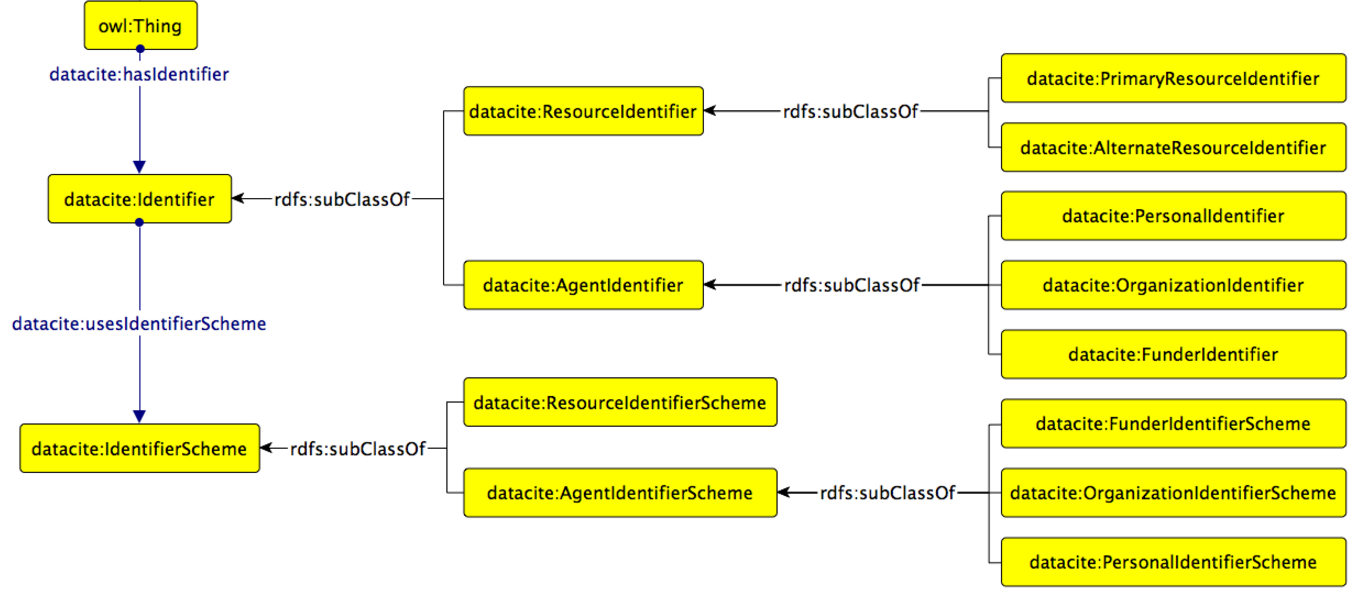
\includegraphics[width=\textwidth]{images/DataCiteIdentifiers.png}
  \caption{DataCite Identifier and IdentifierScheme \cite{Peroni2016}}
  \label{fig:dcid}
\end{figure}

\subsection{re3data.org}
\label{sec:re3data}

The re3data\footnoteurl{http://www.re3data.org/} registry currently lists over 1.600 research repositories, making it the largest and most comprehensive registry of data repositories available on the web. By providing a detailed metadata description of repositories, the registry helps researchers, funding bodies, publishers and research organisations to find an appropriate data repository for different purposes\cite{PAMPLE2013}. Initiated by multiple German research organisations, funded by the German Research Foundation\footnoteurl{http://www.dfg.de/} from 2012 until 2015, re3data is now a service of DataCite\footnoteurl{https://www.datacite.org/}. 
In 2014 re3data merged with the DataBib registry for research data repositories into one service\footnoteurl{http://www.re3data.org/tag/databib/}. 
The re3data project was initiated by the Library and Information Services section (LIS) of the German Research Centre for Geosciences (GFZ), the library of the Karlsruhe Institute of Technology (KIT) and the Berlin School of Library and Information Science (BSLIS) at Humboldt-Universität zu Berlin.

One central goal of re3data is to enhance the visibility of existing research data repositories and to enable all those who are interested in finding a repository to assess a respective information service. This is achieved by an extensive and quality approved metadata description of the listed research data repositories. The basis for this description is the “Metadata Schema for the Description of Research Data Repositories”, having 42 properties in the current version 3.0~\cite{r3dSchema}.

\subsection{Data Lifecycle Ontology (DLO)}
\label{sec:dlo}
The Data Lifecycle Ontology\footnoteurl{https://w3id.org/dlo} provides a set of conceptual entities, agents, activities, and roles to represent the general data engineering process. Furthermore, it is the basis
for deriving specific domain ontologies which represent life-cycles of
data engineering projects such as \dbpedia. With the incorporation of DLO into the \ecosystem, \textit{Activities \& Plans} facilitates a basis for the information exchange needed of combined software and (big) data engineering \cite{SolankiBFKDB16}.

\subsection{The Organization Ontology (ORG)}
\label{sec:org}
The Organization Ontology\footnoteurl{https://www.w3.org/TR/vocab-org/} "[...] describes a core ontology for organizational structures, aimed at supporting linked data publishing of organizational information across a number of domains. It is designed to allow domain-specific extensions to add classification of organizations and roles, as well as extensions to support neighbouring information such as organizational activities." \cite{ReynoldsOrg} \org is a W3C recommendation and provides the backdrop of organisational structures to any given domain.

\subsection{DBpedia}
\label{sec:dbpedia}

\dbpedia is a community effort to extract structured information from \wikipedia and to make this information available on the Web\footnoteurl{http://dbpedia.org}, where it is used as a common point of reference for interlinking and enriching most of the structured data on the Web today, establishing it as the center of the so called 'LOD cloud\footnoteurl{http://lod-cloud.net}',

The main focus of the \dbpedia extraction lies in mapping of info boxes, templates and other easily identified structured data found in \wikipedia articles to properties of the \dbpedia ontology, reflecting the relations and classifications found within \wikipedia \cite{dbpedia}. Together with the mappings to the \wikipedia XML templates, this ontology is curated by a community of interested people around the world to update schematic changes in time for the bi-yearly \dbpedia releases. 

Each release consists of around one hundred datasets for each of its 130 (2016) language editions (reflecting most of the languages of \wikipedia). Datasets are often created around particular properties (such as \prop{rdf:type}) or other distinguishing features. To reflect this large corpus of structured data, the need for specific demands on its metadata is self-evident.


\section{Extensibility and Interoperability} 
\label{sec:extensinter}

This section is dedicated to a discussion on Extensibility and Interoperability. Both concepts are of significant import to this thesis and are therefore discussed here in detail. In the context of metadata schemata, both tend to influence the respective other concept eminently.

\subsection{Extensibility}
\label{sec:extensibility}

An extensible ontology is a well-designed ontology. Thomas Gruber elevated "Extendibility"  into his list of design criteria for ontologies:

\begin{quote}
"An ontology should be designed to anticipate the uses of the shared
vocabulary. It should offer a conceptual foundation for a range of anticipated tasks,
and the representation should be crafted so that one can extend and specialize the
ontology monotonically. In other words, one should be able to define new terms for
special uses based on the existing vocabulary, in a way that does not require the
revision of the existing definitions." \cite{Gruber}
\end{quote}

G{\'{o}}mez{-}P{\'{e}}rez defines this term slightly different:
\begin{quote}
"The expandability of an ontology [...] is a measure of the cost and effort required, in order to extend the ontology by new definitions." \cite{GomezPerez}
\end{quote}

The trait of Extensibility is of high importance to metadata vocabularies. To successfully depict a domain with a metadata vocabulary, a suitable extension of the provided axioms is often necessary, to reflect the peculiarities of a given scenario.
Extending an ontology has multiple advantages in contrast to creating a vocabulary from scratch, which is laid out in this paper \cite{Keet}.

\subsection{Interoperability}
\label{sec:interoperability}
\begin{quote}
"It is becoming generally accepted in the information community that interoperability is one of the most important principles in metadata implementation. [...] From the very beginning of a metadata project, the principles that enable user-centered and interoperable services should be foremost in design and implementation." \cite{3dchinauslibraryconference}
\end{quote}
Many attempts have been made to define the concept of Interoperability:
\begin{quote}
"[...] the ability of
multiple systems with different
hardware and software platforms,
data structures, and interfaces to
exchange data with minimal loss of
content and functionality." \cite{NISO2004}
\end{quote}

\begin{quote}
"[...] the compatibility of two or more systems such that they can exchange information and data and can use the exchanged information and data without any special manipulation." \cite{taylor}
\end{quote}

Haselhofer \& Klas offer a definition for metadata Interoperability based on their survey of techniques for achieving metadata interoperability:

\begin{quote}
"Metadata interoperability is a qualitative property of metadata
information objects that enables systems and applications to work with or use
these objects across system boundaries." \cite{Haslhofer2010}
\end{quote}

The notion of Interoperability can be further delineated: Tolk \cite{Tolk} presented a revised version of the 'Levels of Conceptual Interoperability Model' comprised of: 

\begin{enumerate}
\item no interoperability 
\item technical interoperability (communication infrastructure established) 
\item syntactic interoperability (common structure to exchange information)
\item semantic interoperability (common information model)
\item pragmatic interoperability (context awareness)
\item dynamic interoperability (ability to comprehend state changes) 
\item conceptual interoperability (fully specified, but implementation independent model)
\end{enumerate}

OWL-based metadata is capable of establishing pragmatic Interoperability between two systems (i.e. transferring the intent of the author to the consumer by portraying the same contextual details available to the author). This is a theoretical feature and in practice not easy to achieve. However, providing well-defined and detailed (and machine-readable) resources elevates metadata vocabularies over the mere ability to provide semantic Interoperability.

Different approaches exist to achieve Interoperability between two metadata formats. Chan \cite{3dchinauslibraryconference} describes seven approaches: Uniform standard, Application profiling, Derivation, Crosswalk/mapping, Switching schema, Lingua franca and a Metadata framework, which are not mutually exclusive. Haselhofer \& Klas delineate four main techniques: Model Agreement, Meta-Model Agreement, Model Reconciliation and Metadata Mapping \cite{Haslhofer2010}.
Where Metadata Mapping subsumes both schema and instance level mapping of the Model Reconciliation approach, under the assumption that all metadata information is expressed in the same schema definition language (making the reconciliation at a language level redundant).

\subsection{Extensibility vs. Interoperability}
\label{sec:extensvsinter}
When regarding the definitions of Extensibility and Interoperability, taking into account the intricate requirements of many use cases (such as in \Cref{chap:dmp}), Extensibility and Interoperability seem contradictory when leaving the more general levels of a domain description. A vocabulary capable of interacting with other metadata vocabularies might be too general to fit certain scenarios of use. Restrictive extensions to a vocabulary might encroach on its ability to translate into other useful metadata formats. 

This discrepancy was already described by Gruber, who noted an obvious contradiction between Extensibility on the one hand and ontological commitment\footnote{ontological commitment is the measure of how specialized an ontology is compared to the weakest theory  - only those terms that are essential to the communication of knowledge consistent with that theory.} on the other:

\begin{quote}
"Another apparent contradiction is between extendibility and ontological
commitment. An ontology that anticipates a range of tasks need not include vocabulary
sufficient to express all the knowledge relevant to those tasks [...]. An extensible ontology may specify a very general theory, but include the representational machinery to define the required specializations." \cite{Gruber}
\end{quote}

Interoperability is very similar to the concept of ontological commitment, as in both cases we can anticipate a set of tasks/properties which are relevant in the other/target domain. The notion of contradiction between Extensibility and Interoperability is also corroborated by Frystyk Nielsen:

\begin{quote}
"Unfortunately evolvability\footnote{I do not differentiate between \evolvability and Extensibility (as done in this source) in the context of this thesis. The discrepancies with Interoperability are true for both concepts. Letting features 'die out' over time does not impact, in my understanding, the aspect of Extensibility.} and interoperability don't work towards the same goal - in fact, they can be considered to be two forces that work against each other." \cite{ivse}
\end{quote}

To find the right blend of both concepts depends on the use case and the target vocabulary (or system) with which to interoperate. The Interoperability between two vocabularies of the same domain tends to increase when the Extensibility of at least one is heightened. A general or upper ontology can more easily interoperate with another ontology.



\newpage\thispagestyle{empty}\null
\newpage
\thispagestyle{empty}
\section*{Disambiguation}
There are multiple interpretations of the word/acronym \dataid depending on the context. It can refer to a \dataid metadata document, the serialisation of a \dataid RDF graph. Such a graph is the result of the appliance of \dataid ontologies to one or more datasets, resulting in a collection of RDF statements based on these ontologies. Or it is used to name an instance of the concept \prop{dataid:DataId}, meaning the entry into a \prop{dcat:Catalog}, the most abstract entity in every \dataid document. 
Furthermore, there is the notion of a \ecosystem, which describes the environment consistent of multiple \dataid ontologies and additional extensions.
I will be explicit and use the terms \dataid document, \dataid graph or \dataid resource (or instance, entity) as well as \ecosystem in the remainder of this thesis. 
\\\\
The following naming regime for keywords is adopted:

Keywords such as \important{MediaType} (and their plural form) refer to instances of concepts with the same name, or named individuals in the \dataid ontologies. This is only true for concepts of ontologies from the \ecosystem. When referring to a \important{Dataset}, an instance of \prop{dataid:Dataset} is addressed and not, for example, the concept with the same name in the \dcat vocabulary. There is one exception: Entity refers to an instance of the concept \prop{prov:Entity} (of the \prov ontology). It is generally used in the context of this document to summarise all instances of concepts in the \core ontology which are subclasses of \prop{prov:Entity}: \prop{dataid:DataId}, \prop{dataid:Dataset} and \prop{dataid:Distribution}.

This measure provides specificity about the subject at hand, without having to define each occurrence anew.

\newpage\thispagestyle{empty}\null

\chapter{The DataID Ecosystem}
\label{chap:ecosystem}

\section{Problem Statement} 
\label{sec:probstat}
%Modularizing the original ontology into multiple layers, making DataID independent to the type of data in the process. By augmenting the core ontology with multiple existing extensions and use case specific additions we underline the capabilities in regard to

The inadequacies of current metadata vocabularies are manifold and diverse (\Cref{sec:dv}). As already introduced (\Cref{sec:motivation}), there are some issues which protrude from the rest, due to their ubiquitousness in use cases or their import on aspects like interoperability, trustworthiness and governance of data.

This list of important aspects of metadata reflects these issues and explains them in detail. In the course of this theses I will take particular care to resolve these issues thoroughly.

\textbf{(A1) Provenance}: a crucial aspect of data, required to assess correctness and completeness of data conversion, as well as the basis for the trustworthiness of the data source (no trust without provenance). 

\textbf{(A2) Licensing}: machine-readable licensing information provides the possibility to automatically
%process, integrate and publish 
publish, distribute and consume only data that explicitly allows these actions. 

\textbf{(A3) Access}: publishing and maintaining
this kind of metadata together with the data itself serves as
documentation benefiting the potential user
of the data as well as the creator by making it discoverable
and crawlable. 

\textbf{(A4) Extensibility}: extending a given core metadata model
in an easy and reusable way, while leaving the original model uncompromised expands its application possibilities fitting many
different use cases. 

\textbf{(A5) Interoperability}: the interoperability with other metadata models is a hallmark of a widely usable and reusable metadata vocabulary. It is a prerequisite for uniform access to digital resources on the Web.

Based on the issues explored in \Cref{sec:dv} and the important aspects of dataset metadata above, I conclude, not only is there a gap between existing dataset metadata vocabularies and requirements thereof, but it seems unlikely that one will be able to solve all these diverse problems with just one, monolithic ontology.

%We conclude, that a gap exists between existing dataset metadata vocabularies and what is required.
%Hence it seems unlikely that we are able to solve all these diverse problems with just a single, monolithic ontology.
%Extending a vocabulary for a certain use case will in most cases result in singular, non reusable solutions to a problem. Restrictive extensions of metadata 


\section{The multi-layer ontology of DataID} 
\label{sec:multilayer}

\begin{quote}
"Metadata modularity is a key organizing principle for environments characterized by vastly diverse sources of content, styles of content management, and approaches to resource description. It allows designers of metadata schemas to create new assemblies based on established metadata schemas and benefit from observed best practice, rather than reinventing elements anew." \cite{MetadataPrinciples}
\end{quote}

While trying to solve the different aspects I discussed in the previous section, and tending to the needs of different usage scenarios, the DataID ontology grew in size and complexity (extending \dataid Version 1.0.0 - cf. \Cref{sec:dataid100}).
In order to keep the \dataid ontology reasonable in size and complexity as well as not to jeopardise Extensibility and Interoperability (cf. \Cref{sec:extensvsinter}), I modularised \dataid in a core ontology and multiple extensions. The onion-like layer model (\Cref{fig:onion}) illustrates the import dependencies between the ontologies: 

\begin{figure}[!htbp]
\centering
  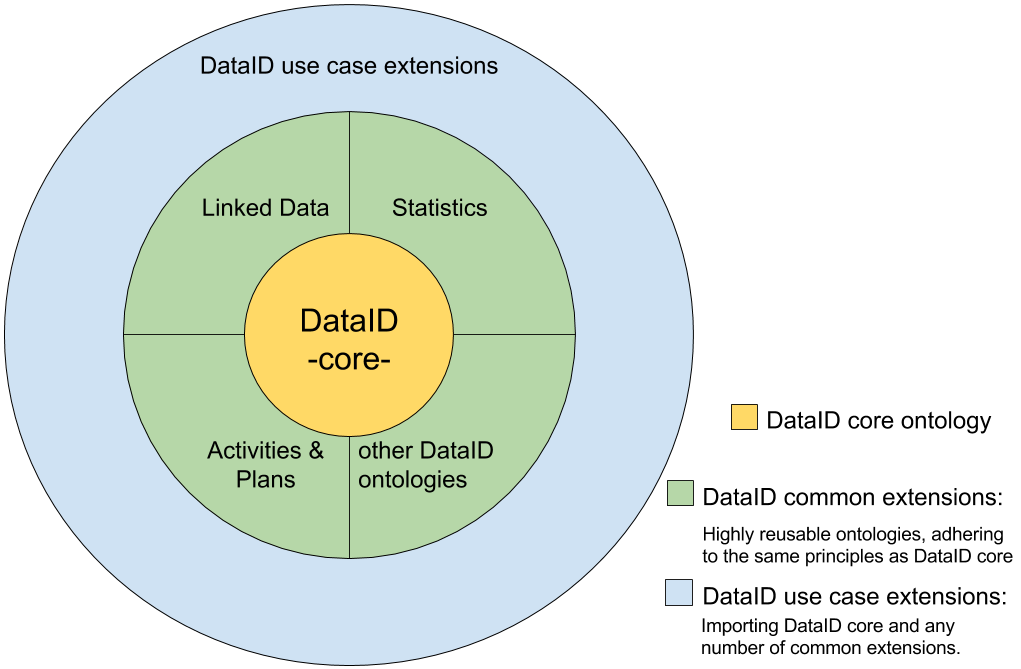
\includegraphics[width=\textwidth]{images/DataIDonion.png}
  \caption{The Metadata Ecosystem of DataID}
  \label{fig:onion}
\end{figure}

The scaling approach used to modularize the original \dataid ontology adopts principles of the modular programming technique, separating concepts and properties of a large ontology into independent, interchangeable modules, specialised to fit common use cases, dependent only on \core. Thus, any vocabulary in this sphere must import \core, with the exception of \core itself. 
The mid-layer (or common extensions) of this model is comprised of highly reusable ontologies, extending \core to cover additional aspects of dataset metadata. None of these are mandatory imports for any ontology, yet, in many cases, some or all of them will be useful contributions. While I will not (and can not) impose any restrictions as to which ontologies not to import, ideally, ontologies of this layer should only import \core, to minimise discrepancies between mid-layer ontologies of different authors with overlapping purposes. The outermost layer of this sphere represents all vocabularies importing \core and any number if mid-layer ontologies and adding additional semantics to portray domain or use case-specific demands for metadata.

Ontologies under the DataID multilayer concept usually do not offer cardinality restrictions, making them easy to extend and adhere to OWL profiles (cf. also \Cref{sec:coreintro}). An application profile, featuring restrictions like cardinalities for the \dataid service stack, which is beeing developed at the moment (cf. \Cref{chap:future}), was declared using SHACL \cite{shacl}.

\section{DataID Extensions of the Common Layer} 
\label{sec:extensions}
The \ecosystem is a suite of ontologies comprised of \core and its extensions, which were created to satisfy different use cases in a reusable manner. \core specifies the basic description of a dataset and serves as a foundation for all extensions to \dataid. While the next chapter provides a detailed introduction to \core (cf. \Cref{chap:core}), this section offers a short overview of the already established landscape of extensions in the common layer of the \ecosystem.
%The brackets enclosed namespace prefixes are recommended and used throughout this work:


\subsection{Linked Data} 
\label{sec:extlinkeddata}

The Linked Data extension (prefix: dataid-ld) extends DataID core with an interface for the SPARQL Service Description vocabulary \cite{sparqlsd}, which not only allows specifying SPARQL endpoints but offers properties useful for Linked Data datasets as well (such as \prop{sd:defaultGraph})\footnoteurl{https://github.com/dbpedia/DataId-Ontology/tree/master/ld}.
A specialised sub-class of \prop{dataid:Dataset} and \prop{sd:Dataset} was introduced to better represent this type of data (\prop{dataid-ld:LinkedDataDataset}). While the \void vocabulary is already imported in \core (cf. \Cref{sec:coreintro}), many \void and properties only become useful in this context (e.g. \prop{void:triples}). In addition to the \prop{void:Linkset} class, describing the relation between datasets, where one holds links to instances of the other, the statistical properties from \void about entities in a Linked Data dataset are of interest (e.g. \prop{void:distinctObjects}).

\subsection{Activities \& Plans} 
\label{sec:extactivitiesplans}
Activities \& Plans extension (prefix: \prop{dataid-acp}) provides provenance information of activities which generated, changed or used datasets\footnoteurl{https://github.com/dbpedia/DataId-Ontology/tree/DataManagementPlanExtension/acp}. The goal is to record all activities needed to replicate a dataset as described by a DataID graph. 
Instrumental to this effort is the further qualification of \prop{prov:wasAttributedTo} property, pointing out agents responsible for activities which transform datasets.
Plans can describe which steps (activities, precautionary measures) are put in place to reach a certain goal (such as a final dataset, data preservation tasks, etc). This extension relies heavily on the \prov ontology and incorporates the Data Lifecycle Ontology (cf. \Cref{sec:dlo}) of the ALIGNED project \cite{SolankiBFKDB16}. A more detailed summary of this extension (incl. \Cref{fig:acp}) is available in \Cref{sec:dmpmodel}.

\subsection{Other DataID ontologies} 
\label{sec:extothers}
More extension ontologies, of similar general character as the ontologies of this layer, are already under way but are not officially released at the moment of writing.

\begin{description}
\item[Statistics (dataid-md)] will provide the necessary measures to publish metadata about multi-dimensional data, such as statistics about datasets, based on the Data Cube Vocabulary\cite{datacube}. 
\item[Data Quality (dataid-dq)] based on the Data Quality Vocabulary \cite{dqv}, this extension is only concerned with quality measurements of the datasets published, closing a evident gap in the current \dataid metadata landscape.
\item[MediaType Vocabulary (dataid-mt)] is currently a namespace used to collect instances of \prop{dataid:MediaType} to reuse them more easily. An full extension on the matter of more intricate depiction of media types (cf. \Cref{sec:coremediatype}) is also planned.
\end{description}


\section{The landscaping approach of the DataID Ecosystem} 
\label{sec:landscaping}

Multiple requirements are planned to be enforced for the adoption of new ontologies into the common (or mid) layer of the DataID Ecosystem.
They might contain (while not being restricted to):

\begin{itemize}
\item Authors must provide information about the reason for the new extension (and why the expected result is not achievable with existing extensions).
\item Authors must document the Interoperability with other extensions of this layer (and where problems (such as semantic overlap) are to be expected).
\item Authors must inform about conformity with OWL profiles.
\end{itemize}

The semantic regulations of interrelations between \dataid ontologies are not yet finalised and are subject of further discussion. The general idea is to provide a controlled environment, in which the interplay of different extensions and \core is regulated, or at least sufficiently documented. Thus, providing a structured approach to combining multiple ontologies for a particular purpose, without having to be aware of every individual axiom. Possible side effects of combining two ontologies would be dealt with, or brought to the user's attention, by the authors of the involved extensions. This concept is my proposal of providing much-needed landscaping between ontologies, to confront such problems as detected in \cite{feeney2015linked}.

A useful tool to help integrate multiple ontologies is the Dacura Data Curation System\footnoteurl{http://dacura.cs.tcd.ie}. It provides the Dacura Quality Service, "[...] which is designed to consume OWL and RDF linked data schemata and identify potential problems in their specifications.
This reasoner uses a much less permissive
interpretation than that of standard OWL to find issues
which are likely to stem from specification errors,
even in cases where they produce valid OWL models." \cite{Feeney16} 
Such an approach is imperative to prevent logical and practical problems between different ontologies (cf. \Cref{sec:motivation}).

Furthermore, extending this ecosystem of dataset metadata with domain-specific OWL ontologies adds further opportunities for applications clustered around datasets. I will demonstrate the methodology of working with these ontologies to satisfy the metadata requirements of complex use cases in a best practice (\Cref{sec:composingmetadata}) as well as an application of these practices in \Cref{chap:dmp}.

\chapter{DataID core Ontology}
\label{chap:core}

\section{Overview} 
\label{sec:coreintro}

This section will provide an overview of the \core ontology and some background on basic design decisions made. Most of the vocabularies reused by this ontology have already been presented in \Cref{chap:relatedwork} and need no further introduction.

\core developed out of a previous version of \dataid (cf. \Cref{sec:dataid100}) by following the aspiration to modularise \dataid into a core-ontology, surrounded by its dependents. Many design decisions of \core were already introduced in its former version, which was designed to make \dcat, combined with the \void and \prov vocabularies, fit the requirements of the \dbpedia use case for a hierarchy of Linked Data datasets (cf. \Cref{sec:dbpedia}).

\begin{quote}
"The DBpedia dataset, with
its different versions and languages, multiple SPARQL endpoints
and thousands of dump files with various content
serves as one example of the complexity metadata models
need to be able to express. We argue that the DCAT vocabulary
as well as the established VoID vocabulary only
provide a basic interoperability layer to discover data. In
their current state, they still have to be expanded to fully
describe datasets as complex as DBpedia [...]." \cite{dataID2014} 
\end{quote}

\core is founded on two pillars: the \dcat and \prov ontologies. To incorporate \dcat as the basis of \dataid, to further extend \dcat with \prov, introducing extensive provenance records in the process, and adding properties specific to the \dbpedia use case was the original premise of this endeavour. Also, the \void vocabulary was adopted to cover Linked Data specific semantics and provide more general properties, such as  \prop{void:subset} for establishing dataset hierarchies. The wide application of these vocabularies in the context of the Semantic Web was the rationale behind these decisions, furthering the goal of Interoperability. 

\begin{figure}[!htbp]
\centering
  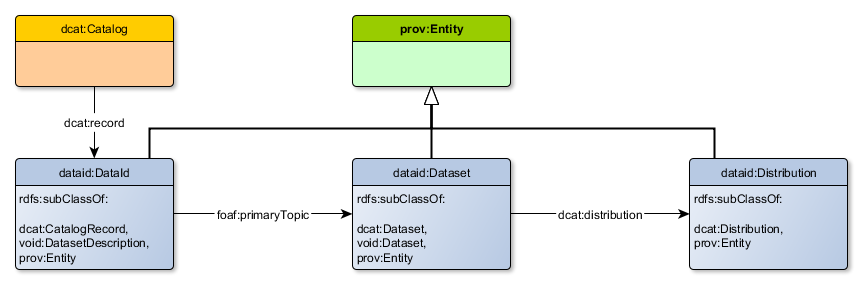
\includegraphics[width=\textwidth]{images/FoundationalConcept.png}
  \caption{Foundations: Combining \dcat, \void and \prov}
  \label{fig:foundations}
\end{figure}

\core is centred around the dataset and distribution concepts which were imported from \dcat. I introduced the class \prop{dataid:DataId} (cf. \Cref{sec:coredataid}), merging both \prop{dcat:CatalogRecord} and \prop{void:DatasetDescription} into one, providing an additional level of abstraction between the conscepts of dataset and catalogue. Instances of this class can be compared to root elements in the XML documents, since all subsequent instances, describing a \important{Dataset}, are hierarchically below a \important{DataId} instance. Though, this comparison is of course misleading, since a graph has no orientation. Nevertheless, most of DataID documents\footnote{a DataID graph serialised as a metadata document} will have structural similarities to XML documents.

All dataset related classes of \core (\prop{dataid:DataId}, \prop{dataid:Dataset} and \prop{dataid:Distribution}) are sub-classes of \prop{prov:Entity}, which is the interface needed to harness the possibilities of the Provenance Ontology (\prov). In the context of this description of \core, the word 'Entity' is used to refer to instances of \prop{prov:Entity} (ergo: instances of these three classes).

With \prov, describing the circumstance of provenance for any domain is possible (\Cref{sec:prov}). Central to this, is the concept of qualification classes, providing qualifications for more general properties (e.g. for \prop{prov:wasAttributedTo}). Describing the interrelations between \important{Entities} (such as a particular \important{Dataset} or just a single \important{Distribution} of it) and \important{Agents} (e.g. a person or an organisation) are salient requirements in most environments for datasets and their metadata. Thus, \core has singled out these relations to further qualify them and provide much needed referential integrity.
\todo{explain}

For example, the property \prop{dataid:associatedAgent} (which is a sub-property of \prop{prov:wasAttributedTo}) is a universal relation between an \important{Entity} and an \important{Agent}. It can (and should) be qualified by an instance of \prop{dataid:Authorization}, a sub-class of \prop{prov:Attribution}. An \important{Authorization} adds qualifications and restrictions to the original property, such as an agent role (defining the role the \important{Agent} has in regard to the \important{Entities} involved - see \Cref{sec:coreauthorization}). \core allows for assigning Actions to an \important{Authorization}, which specify what an \important{Agent} can do and for which tasks an \important{Agent} is responsible.

\begin{figure}[!htbp]
\centering
  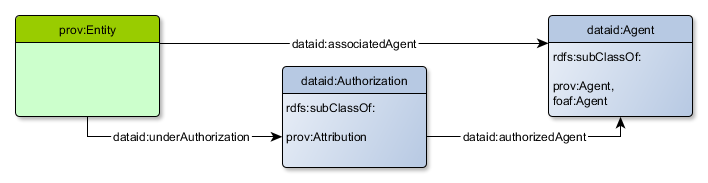
\includegraphics[width=\textwidth]{images/FoundationalConseptProv.png}
  \caption{Foundations: Using \prov to qualify properties}
  \label{fig:foundations}
\end{figure}

In its current version 2.0.0, \core offers a general approach for describing dataset metadata, incorporating important ontologies to extend \dcat with Provenance, qualifying relations and their intended range classes, hierarchical dataset structures, management of rights and responsibilities of \important{Agents} and exhaustive descriptions for data Access. 

In general, \core forbore the use of cardinality restrictions\footnote{this is the purpose of an application profile, not of an ontology}, making it easier to adhere to the OWL 2 RL (cf. \Cref{sec:owl}) profile and maintaining the benefits of easy Extensibility and Interoperability prevalent with \dcat. In turn, \core restricts some of the very general property ranges of Dublin Core and \dcat properties (such as \prop{dct:license} or \prop{dcat:mediaType}), to reduce impreciseness and increase machine-readability.

\core is making use of the following namespace:
\begin{lstlisting}[language=ttl, label=lst:graph,linewidth=\columnwidth,breaklines=true,basicstyle=\ttfamily\footnotesize]
http://dataid.dbpedia.org/ns/core#
\end{lstlisting}
At this URI, an extended description of each class and property, introduced by this ontology, can be found as well as the complete ontology specification in Turtle\footnoteurl{http://dataid.dbpedia.org/ns/core.ttl} or OWL\footnoteurl{http://dataid.dbpedia.org/ns/core.owl} serialisation. The current version is available in Appendix I.

For a better understanding of the imported concepts and properties, which are reused by \core, I would advise to read up on \dcat \cite{ddcat} and \prov \cite{prov} (since these are used most commonly), to gain a more complete picture of the underlying structure and rationale of these ontologies. While I gave a concise introduction to both in \Cref{sec:dcat} and \Cref{sec:prov} respectively, this work is not the place to repeat this in more detail.

\begin{figure}
\centering
	\vspace*{-0.8cm}
  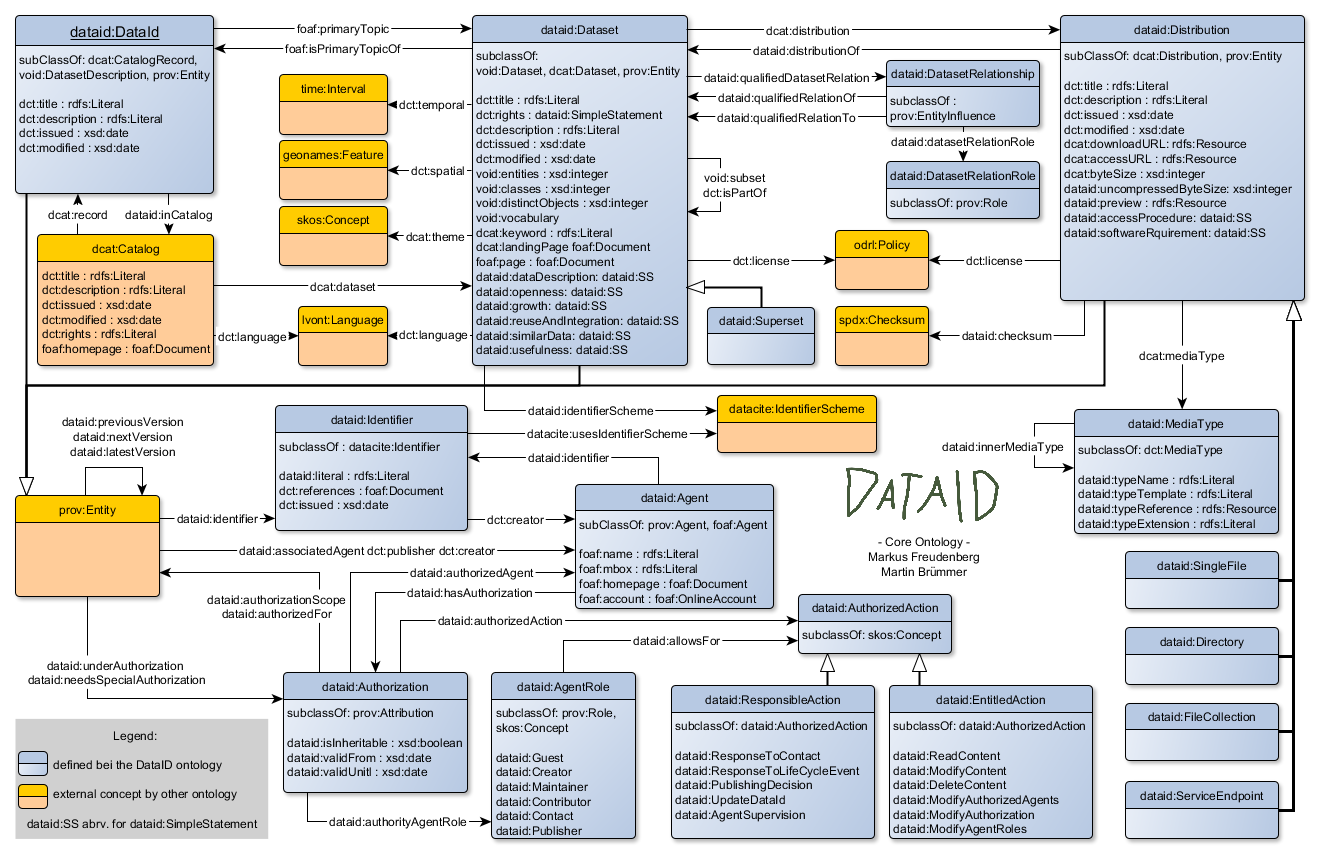
\includegraphics[angle=90, width=\textwidth]{images/DataIdOntology.png}
  \caption{\core}
  \label{fig:core}
  %\floatfoot{An exact description of all classes and properties can be found under the DataID namespace uri \url{http://dataid.dbpedia.org/ns/core} including this depiction. The ontology RDF document is also available there:
  %\url{http://dataid.dbpedia.org/ns/core.ttl} (.owl)}
\end{figure} 

\pagebreak
\section{Classes} 
\label{sec:coreclasses}

This section is partitioned by concepts to introduce the \core ontology. Each class is presented with an item of written comment about the general reasoning behind its existence and its intended use.
For illustration purposes, a running example was woven into the descriptions of concepts and properties. This example is a reduced version of an original \dataid document of the Arabic \dbpedia (release: 2015-10\footnoteurl{http://vmdbpedia.informatik.uni-leipzig.de/dataid-w3c-submission/html/2015-10_dataid_ar.ttl}). Under the main \important{Dataset}, only two \important{Sub-Datasets} are shown (as opposed to over 50 in the real world example from which this is drawn). Each Dataset has two distributions for two different RDF serialisations (Turtle '.ttl' and Quad-Turtle '.tql'). One is also represented by the official \dbpedia SPARQL endpoint.
This example was chosen to cover many aspects of \core and to provide an easy use case which could arise in a similar fashion outside the \dbpedia domain. The full example is available in \textit{Turtle} serialisation\footnoteurl{https://www.w3.org/TeamSubmission/turtle/} in Appendix II. The basic structure of its \dataid document is outlined below (\Cref{fig:example}).

\begin{figure}[!htbp]
\centering
  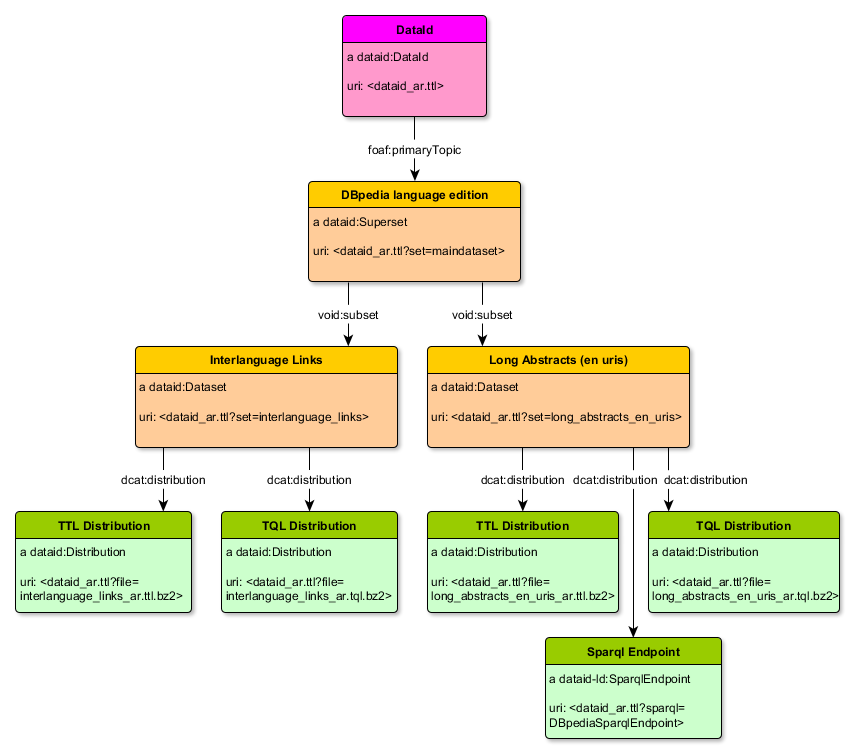
\includegraphics[width=\textwidth]{images/ExampleStructure.png}
  \caption{A shallow dataset hierarchy of the Arabic DBpedia language edition.}
  \label{fig:example}
\end{figure}

For the purpose of this running example the following base URI was used to shorten all subsequent URIs:
\begin{lstlisting}[language=ttl,label=lst:graph,linewidth=\columnwidth,breaklines=true,basicstyle=\ttfamily\footnotesize]
@base <http://downloads.dbpedia.org/2015-10/core-i18n/ar/2015-10_>
\end{lstlisting}

The example often omits the more common properties of Dublin Core (cf. \Cref{sec:metadata}) and \rdfs (cf. \Cref{sec:owl}) such as \prop{dct:title}, \prop{dct:description}, \prop{dct:modified}, \prop{dct:issued} and \prop{rdfs:label} to make this example more easy to read. 

In addition, this running example does not only use \core, but it also introduces a first \dataid extension from the common layer of the \ecosystem (\Cref{sec:multilayer}) for Linked Data datasets. The Linked Data extension\footnoteurl{https://github.com/dbpedia/DataId-Ontology/tree/master/ld} (prefix: dataid-ld) is used to describe dataset attributes, specific to Linked Data.

The remainder of this section features each subsection with a summary, stating the purpose of each concept, a list of properties commonly used to describe instances of this concept, a schematic depiction of the concept, followed by at least one example instance of this class (taken from the running example of \dbpedia). The list of properties features a rating for each property to advise whether an application profile based on \core should declare a property to be: mandatory \textbf{(M)}, recommended \textbf{(R)} or optional \textbf{(O)} (again: this is only a recommendation, \core does not provide cardinality restrictions).


\subsection{DataId} 
\label{sec:coredataid}
The class \prop{dataid:DataId} inherits from \prop{dcat:CatalogRecord} and \prop{void:DatasetDescription}, which does not represent a dataset, but metadata about a dataset's entry in a catalogue. Additionally, in the context of \core, it represents metadata about a \dataid document (or the graph serialised in it), such as version pointers, modification dates and relations to contextual \important{Entities} (agents, catalogues, repositories). This \dataid resource is the most abstract \important{Entity} in any \dataid graph. 

\begin{figure}[!htbp]
\centering
  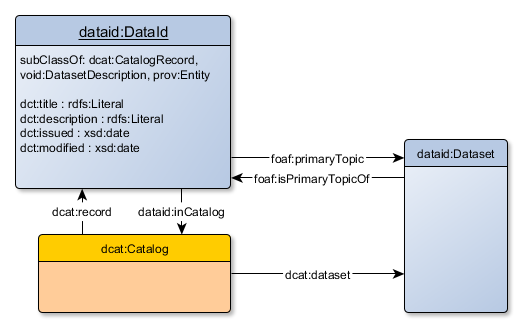
\includegraphics[width=10cm]{images/ClassDataId.png}
  \caption{The DataId concept}
  \label{fig:example}
\end{figure}

Properties specifically used with \prop{dataid:DataId}:
\begin{description}
\item[\prop{dataid:inCatalog}:] the inverse of \prop{dcat:record} references the \dcat catalogue a \dataid is entered in. \hfill\textbf{(R)}
\item[\prop{foaf:primaryTopic}:] this functional property is used to point out the \important{Dataset} resource this \dataid represents. \hfill\textbf{(M)}
\end{description}

Additionally, the following list contains properties which can be used with any sub-class of \prop{prov:Entity}, presented only for this concept out of convenience:
\begin{description}
\item[\prop{dataid:associatedAgent}:] points out all \important{Agents} which have some (unspecified) influence (or authority) over this \important{Entity}. \hfill\textbf{(O)}
\item[\prop{dataid:underAuthorization}:] refers to an instance of \prop{dataid:Authorization} which qualifies the generic \prop{dataid:associatedAgent} relation (cf. \Cref{sec:coreauthorization}). \hfill\textbf{(R)}
\item[\prop{dct:publisher}:] While the \prov based way to declare associated \important{Agents} and their roles in regard to an \important{Entity} is in place, using established properties to point out \important{Agents} (such as \prop{dct:publisher} of \prop{dcat:contactPoint}) is not redundant and should be kept as best practice. \hfill\textbf{(R)}
\item[\prop{dataid:identifier}:] similar to \important{Agents}, \important{Entities} often have unique identifiers defined for them in a different context (in addition to the URI used in the context of a \dataid document). This property points out additional identifiers (cf. \Cref{sec:coreidentifier}). \hfill\textbf{(O)}
\item[\prop{dataid:nextVersion}:] is used to identify instances of the same type (in this case \prop{dataid:DataId}), which are next in the chain of different versions of this resource. \hfill\textbf{(O)}
\item[\prop{dataid:previousVersion}:] points out the previous version of this instance. \hfill\textbf{(R)}
\item[\prop{dataid:latestVersion}:] points out the latest version of this instance. \hfill\textbf{(R)}
\end{description}

The example below illustrates the use of this concept. It provides a pertaining dataset catalogue (via \prop{dataid:inCatalog}), uses version pointers to define its position in a branch of a versioning system, points out \important{Agents} and \important{Authorizations}, and the \important{Dataset} this \dataid is about (\prop{foaf:primaryTopic}).
\\
\begin{lstlisting}[language=ttl, captionpos=b,caption=Instance of a DataId,label=lst:coredataid,linewidth=\columnwidth,breaklines=true]
<dataid_ar.ttl>
        a                          dataid:DataId ;
        dataid:associatedAgent     <http://wiki.dbpedia.org/dbpedia-association> ;
        dataid:inCatalog           <http://downloads.dbpedia.org/2015-10/2015-10_dataid_catalog.ttl> ;            
        dataid:latestVersion       <http://downloads.dbpedia.org/2016-04/core-i18n/ar/2016-04_dataid_ar.ttl> ;
        dataid:nextVersion         <http://downloads.dbpedia.org/2016-04/core-i18n/ar/2016-04_dataid_ar.ttl> ;    
        dataid:previousVersion     <http://downloads.dbpedia.org/2015-04/core-i18n/ar/2015-04_dataid_ar.ttl> ;
        dataid:underAuthorization  <dataid_ar.ttl?auth=creatorAuthorization> ;                                    
        dct:hasVersion             <dataid_ar.ttl?version=1.0.0> ;
        dct:publisher              <http://wiki.dbpedia.org/dbpedia-association> ;                                
        dct:title                  "DataID metadata for the Arabic DBpedia"@en ;
        foaf:primaryTopic          <dataid_ar.ttl?set=maindataset> .
\end{lstlisting}

\pagebreak
\subsection{Dataset} 
\label{sec:coredataset}
This is the central concept of the \core ontology and offers a multitude of useful properties to describe a dataset comprehensively.
\begin{figure}[!htbp]
\centering
  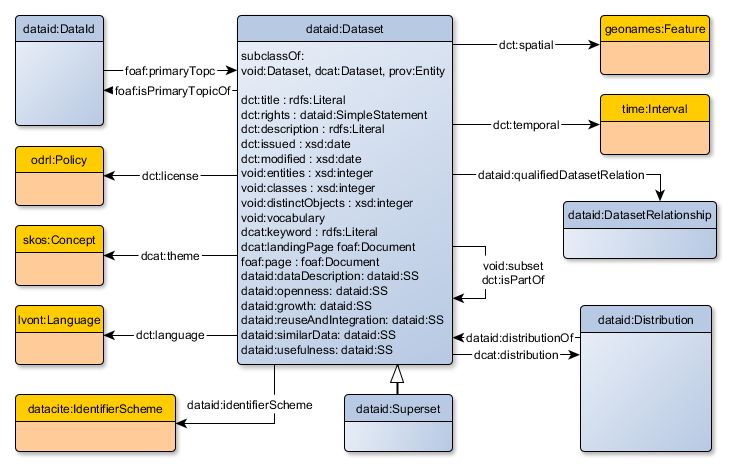
\includegraphics[width=\textwidth]{images/ClassDataset.png}
  \caption{The Dataset concept}
  \label{fig:example}
\end{figure}

The dataset concept of both the \dcat and \void vocabularies were merged into \prop{dataid:Dataset}, providing useful properties about the content of a \important{Dataset} from both ontologies. In particular, the property \prop{void:subset} allows for the creation of dataset hierarchies, while \prop{dcat:distribution} points out the \important{Distributions} of a \important{Dataset}. The \prop{dataid:Superset} as a subclass of \prop{dataid:Dataset} shall be used to represent multiple \important{Sub-Dataset}, representing dataset collections or hierarchical dataset structures in general. Opposed to a conventional \important{Dataset}, a \important{Superset} is prohibited from possessing \important{Distributions} (referred to with \prop{dcat:distribution}). It is strongly recommended that each \important{Dataset} shall either have at least one \important{Distribution} or one \important{Sub-Dataset}. 

In the running example, the main \important{Dataset} (an instance of \prop{dataid:Superset}), is used as a hierarchical top entity, representing all \important{Sub-Datasets} clustered around a common topic. In the case of \dbpedia, all \important{Datasets} were arranged under a \important{Superset} representing a \dbpedia language edition.

Properties commonly used with instances of this class are:
\begin{description}
\item[\prop{dcat:distribution}] provides the \important{Distributions} of a \important{Dataset} and should be used distinct from \prop{void:subset}. \hfill\textbf{(M for non Supersets)}
\item[\prop{void:subset}] is the property used to reference \important{Sub-Datasets} which are part of a \important{Superset}. Its use is limited to \prop{dataid:Superset}. \hfill\textbf{(M if Superset)}
\item[\prop{dct:license}] this property is restricted in the context of \dataid to instances of the class \prop{odrl:Policy} (cf. \Cref{sec:odrl})of the \odrl ontology, providing machine-readable licensing information. \hfill\textbf{(M)}
\item[\prop{dct:language}:] this property from the Dublin Core vocabulary is used to point out the predominant language used within a \important{Dataset}. Since a \prop{rdfs:range} statement is not provided in its original definition, even simple literals could be used with this predicate. \core restricts the range of this property to instances of  \prop{lvont:Language} from the Lexvo ontology (cf. \Cref{sec:lexvo}), describing human languages in a machine readable way. \hfill\textbf{(R)}
\item[\prop{void:vocabulary}] in the \void vocabulary, this property is used to point out the associated ontology used to create a \important{Dataset}. \core broadens its use so that any schema document (e.g. XSD or database schemata) can be pointed out, depending on the type of data. \hfill\textbf{(R)}
\item[\prop{foaf:page}] is commonly used to point out web pages which have the function of a manual or documentation for the resource at hand. \hfill\textbf{(R)}
\item[\prop{dct:rights}] this property is used to provide a statement or resource about issues like copyrights or legal notes. To avoid unqualifiable literal statements, this property is restricted to be used with \prop{dataid:SimpleStatement} (cf. \Cref{sec:simplestatement}). \hfill\textbf{(O)}
\item[\prop{foaf:isPrimaryTopicOf}] is the inverse property of \prop{foaf:primaryTopic} (cf. \Cref{sec:coredataid}). \hfill\textbf{(O)}
\item[\prop{dataid:relatedDataset}:] generic pointer to related \important{Datasets} (sub-property of \prop{dct:relation}), qualifiable by \prop{dataid:qualifiedDatasetRelation}. Refer to \Cref{sec:corerelation} for more. \hfill\textbf{(O)}
\item[\prop{dataid:qualifiedDatasetRelation}] provides an instance of concept \prop{dataid:DatasetRelationship} which is a qualification class for the generic property \prop{dataid:relatedDataset} (cf. \Cref{sec:corerelation}). \hfill\textbf{(O)}
\item[\prop{dataid:identifierScheme}:] provides a resource, describing the identifiers used within the \important{Dataset} to uniquely identify a record (data point, datum). Refer to \Cref{sec:coreidentifier} to learn more about \important{Identifiers}. \hfill\textbf{(O)}
\item[\prop{dcat:keyword}:] a simple keyword or tag associated with this \important{Dataset} \hfill\textbf{(O)}
\item[\prop{dcat:landingpage}:] references a web page of general character (such as the homepage of an organisation) \hfill\textbf{(O)}
\end{description}

Multiple properties for textual statements on different aspects of a \important{Dataset} were created. All of which provide \important{Publishers}, \important{Maintainers} and other \important{Agents} a way to convey statements of general character on such subjects as described below. This information will be useful in many scenarios related to dissemination tasks, for example, those described by the Horizon 2020\footnoteurl{https://ec.europa.eu/programmes/horizon2020/} data management plan guidelines\footnoteurl{https://ec.europa.eu/research/participants/data/ref/h2020/grants_manual/hi/oa_pilot/h2020-hi-oa-data-mgt_en.pdf} (see also \Cref{chap:dmp}).

All of these properties listed below have the common \prop{rdfs:range} of \prop{dataid:SimpleStatement}, which allows to either provide a literal or reference a web page containing the textual information about the resource (cf. \Cref{sec:corestatement}). 

\begin{description}
\item[\prop{dataid:dataDescription}:] provides a detailed textual description of the data represented by this \important{Dataset}. \hfill\textbf{(O)}
\item[\prop{dataid:growth}:] an indication of what size the approximated end volume of the \important{Dataset} is. \hfill\textbf{(O)}
\item[\prop{dataid:usefulness}:] is used to state to whom the \important{Dataset} could be useful, and whether it underpins a scientific publication. \hfill\textbf{(O)}
\item[\prop{dataid:similarData}:] a statement on the existence (or absence) of similar data (see also \prop{dataid:relatedDataset}). \hfill\textbf{(O)}
\item[\prop{dataid:reuseAndIntegration}:] information on the possibilities for integration and reuse of the \important{Dataset}. \hfill\textbf{(O)}
\item[\prop{dataid:openness}:] General description of how data will be shared. For example embargo periods (if any), outlines of technical mechanisms for dissemination or a definition of whether access will be widely open or restricted to specific groups. In case the \important{Dataset} cannot be shared, the reasons for this should be mentioned (e.g. ethical, rules of personal data, intellectual property, commercial, privacy-related, security-related). \hfill\textbf{(O)}
\end{description}

\pagebreak
The running example is structured in a shallow hierarchy with an instance of \prop{dataid:Superset} representing all \important{Datasets} of an Arabic \dbpedia language edition:
\\
\begin{lstlisting}[language=ttl, captionpos=b,caption=Instance of a Superset,label=lst:coresuperset,linewidth=\columnwidth,breaklines=true]
<dataid_ar.ttl?set=maindataset>
        a                           dataid:Superset ;
        dataid:associatedAgent      <http://wiki.dbpedia.org/dbpedia-association>  ;
        dataid:growth               <dataid_ar.ttl?stmt=growth> ;                                                 
        dataid:openness             <dataid_ar.ttl?stmt=openness> ;
        dataid:reuseAndIntegration  <dataid_ar.ttl?stmt=reuseAndIntegration> ;
        dataid:similarData          <dataid_ar.ttl?stmt=similarData> ;
        dataid:usefulness           <dataid_ar.ttl?stmt=usefulness> ;
        dct:hasVersion               <dataid_ar.ttl?version=1.0.0> ;
        dct:language                 <http://lexvo.org/id/iso639-3/ara> ;                                          
        dct:license                  <http://purl.oclc.org/NET/rdflicense/cc-by-sa3.0> ;  
        dct:publisher                <http://wiki.dbpedia.org/dbpedia-association> ;
        dct:rights                   <dataid_ar.ttl?rights=dbpedia-rights> ;
        void:subset                 <dataid_ar.ttl?set=long_abstracts_en_uris>, 
        <dataid_ar.ttl?set=interlanguage_links> ;
        void:vocabulary             <http://downloads.dbpedia.org/2015-04/dbpedia_2015-10.owl> ;                  
        dcat:keyword                "maindataset"@en , "DBpedia"@en ;
        dcat:landingPage            <http://dbpedia.org/> ;                                                       
        foaf:isPrimaryTopicOf       <dataid_ar.ttl> ;                                                             
        foaf:page                   <http://wiki.dbpedia.org/Downloads2015-10> .  
\end{lstlisting}

This \important{Dataset} has no \important{Distributions}, the data it represents is referred to via its \important{Sub-Datasets}. As an example for one of its \important{Sub-Datasets}, the following listing exemplifies this difference (use of \prop{dcat:distribution} instead of \prop{void:subset}):
\begin{lstlisting}[language=ttl, captionpos=b,caption=Instance of a Dataset,label=lst:coresuperset,linewidth=\columnwidth,breaklines=true]
<dataid_ar.ttl?set=long_abstracts_en_uris>
        a                       dataid:Dataset, dataid-ld:LinkedDataDataset ;
        dataid:associatedAgent  <http://wiki.dbpedia.org/dbpedia-association> ;
        dataid:qualifiedDatasetRelation   <dataid_ar.ttl?relation=source&target=pages_articles> ;                 
        dataid:relatedDataset   <dataid_ar.ttl?set=pages_articles> ;
        dct:hasVersion           <dataid_ar.ttl?version=1.0.0> ;
        dct:isPartOf             <dataid_ar.ttl?set=maindataset> ;                                                 
        dct:language             <http://lexvo.org/id/iso639-3/ara> ;
        dct:license              <http://purl.oclc.org/NET/rdflicense/cc-by-sa3.0> ;
        dct:title                "long abstracts en uris"@en ;
        void:rootResource       <dataid_ar.ttl?set=maindataset> ;
        void:triples            232801 ;                                                                          
        void:sparqlEndpoint      <http://dbpedia.org/sparql> ;                                                    
        dcat:distribution       <dataid_ar.ttl?sparql=DBpediaSparqlEndpoint> ,                                    
            <dataid_ar.ttl?file=long_abstracts_en_uris_ar.ttl.bz2> ,
            <dataid_ar.ttl?file=long_abstracts_en_uris_ar.tql.bz2> ;
        dcat:keyword            "long_abstracts_en_uris"@en , "DBpedia"@en ;
        dcat:landingPage        <http://dbpedia.org/> ;
        sd:defaultGraph         <http://ar.dbpedia.org> ;                                                         
        foaf:page               <http://wiki.dbpedia.org/Downloads2015-10> . 
\end{lstlisting}

\pagebreak
\subsection{Distribution} 
\label{sec:coredist}

The class \prop{dataid:Distribution} provides the technical description of the data, the 'manifestation' of a \important{Dataset}. In addition, it serves as documentation of how to access the data described (e.g. \prop{dcat:accessURL}), and which conditions apply (e.g. \prop{dataid:accessProcedure}). Every \important{Distribution} of a \important{Dataset} must contain all data of the \important{Dataset} in the format and location described. It may contain additional data exceeding the defined \important{Dataset}, for example when describing a service endpoint. Two \important{Distributions} of the same \important{Dataset}, therefore, must either contain the same data (for example in two different serialisations), or one \important{Distribution} must completely subsume the other. The \important{Distribution} concept, introduced by the \dcat vocabulary, is crucial to be able to automatically retrieve and use the data described in a \dataid document, simplifying, for example, data analysis. Additional sub-classes, to further distinguish how the data is available on the Web, were introduced:

\begin{figure}[!htbp]
\centering
  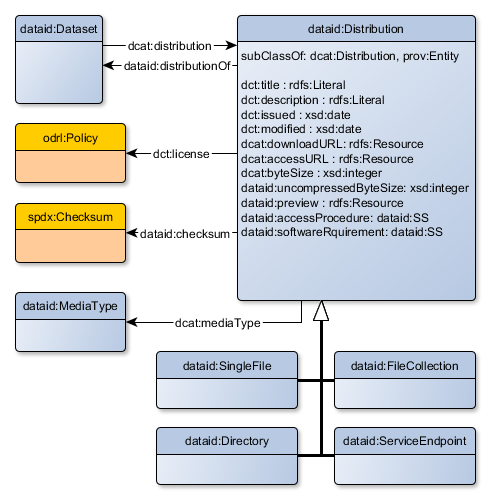
\includegraphics[width=10cm]{images/ClassDistribution.png}
  \caption{The Distribution concept}
  \label{fig:example}
\end{figure}

\begin{description}
\item[\prop{dataid:SingleFile}:] all data of a \important{Dataset} is available in a single file.
\item[\prop{dataid:Directory}:] the data of a \important{Dataset} is represented by the files in a single Directory on a file system.
\item[\prop{dataid:FileCollection}:] an arbitrary collection of (different files, not restricted to one file system), which in their accumulation represent the data of a \important{Dataset}.
\item[\prop{dataid:ServiceEndpoint}:] is a superclass for all service/api endpoints which could provide datasets. For example, REST APIs for databases\footnoteurl{https://docs.oracle.com/cloud/latest/mysql-cloud/CSMCS/index.html} or SPARQL endpoints.
\end{description}

Except for \prop{dataid:SingleFile}, all of these subclasses may need additional semantics to describe them in a useful manner. This is not an objective of \core, further extensions of this ontology will address these issues.

Properties used with \prop{dataid:Distribution}:
\begin{description}
\item[\prop{dcat:mediaType}:] is restricted to a range of \prop{dataid:MediaType} (cf. \Cref{sec:coremediatype}). This property is absolutely necessary to digest the content of a \important{Distribution} automatically. \hfill\textbf{(M)}
\item[\prop{dcat:downloadURL}:] this property supplies a URL under which the described \important{Distribution} can be downloaded directly (without any access procedure or intermediate steps) and completely. \hfill\textbf{(M if no \prop{dcat:accessURL})}
\item[\prop{dcat:accessURL}:] when additional steps are necessary to achieve access to the data of this \important{Distribution} (such as authorisations, querying or selecting data from a repository), \prop{dcat:accessURL} is used to provide the initial URL. If the process necessary to retrieve the data is not evident by the content of the web page referred, publishers should make use of property. \prop{dataid:accessProcedure}. \hfill\textbf{(M if no \prop{dcat:downloadURL})}
\item[\prop{dataid:accessProcedure}:] is used to convey a description of necessary steps, needed to retrieve the data of this \important{Distribution} from the \prop{dcat:accessURL}. This property has the range\prop{dataid:SimpleStatement} and should not be used in connection with \prop{dcat:downloadURL}. \hfill\textbf{(R if no \prop{dcat:downloadURL})}
\item[\prop{dataid:checksum}:] the range of this property is restricted to \prop{spdx:Checksum} \cite{spdx}, providing \prop{spdx:checksumValue} and \prop{spdx:algorithm} properties for an exact definition of a checksum. Checksums can be used to validate the correctness of downloaded files, directories and API endpoint responses. \hfill\textbf{(R)}
\item[\prop{dcat:byteSize}:] The exact size of a \important{Distribution} in bytes. \hfill\textbf{(R)}
\item[\prop{dataid:softwareRequirement}:] Some data formats/serialisations are only useful with a particular software product. This statement offers the possibility to name such circumstances. \hfill\textbf{(O)}
\item[\prop{dataid:uncompressedByteSize}:] Often, files and media streams are compressed to reduce the number of bytes to be transferred. This optional property provides the means to specify the size of the \important{Distribution} in its uncompressed extension. \hfill\textbf{(O)}
\item[\prop{dataid:preview}:] While the exact format and serialisation of the \important{Distribution} is defined by \prop{dataid:MediaType}, it is often beneficial for publishers and consumers to have a look at the actual format of the (uncompressed) data. This property points out a web resource providing such a preview. \hfill\textbf{(O)}
\item[\prop{dataid:distributionOf}:] the inverse property of \prop{dcat:distribution}, pointing back to the \important{Dataset} instance this \important{Distribution} belongs to. \hfill\textbf{(O)}
\item[\prop{dct:license}:] see \Cref{sec:coredataset} for a detailed description. Often, the license used for the \important{Distribution} is the same as for the pertaining \important{Dataset}. For those cases where this is not true, the use of this property in the context of a \important{Distribution} is advised. \hfill\textbf{(O)}
\end{description}

The first example is an instance of \prop{dataid:SingleFile}, describing a single RDF file (which contains the whole \important{Dataset}) in Turtle syntax, compressed with the bzip2 compression\footnoteurl{http://www.bzip.org}. It can be downloaded directly (without any intermediate steps), hence the property \prop{dcat:downloadURL} is used to point out the resource on the Web. Since it is a compressed file, the byte size in its compressed and uncompressed state is provided. An instance of \prop{spdx:Checksum} was included, providing the checksum value for this \important{Distribution}.
\\
\begin{lstlisting}[language=ttl, captionpos=b,caption=Example of a SingleFile Distribution,label=lst:coresuperset,linewidth=\columnwidth,breaklines=true]
<dataid_ar.ttl?file=long_abstracts_en_uris_ar.ttl.bz2>
        a                        dataid:SingleFile ;
        dct:license              <http://purl.oclc.org/NET/rdflicense/cc-by-sa3.0> ;                              
        dct:publisher            <http://wiki.dbpedia.org/dbpedia-association> ;
        dataid:associatedAgent   <http://wiki.dbpedia.org/dbpedia-association> ;
        dataid:checksum          <dataid_ar.ttl?file=long_abstracts_en_uris_ar.ttl.bz2&checksum=md5> ;            
        dataid:isDistributionOf  <dataid_ar.ttl?set=long_abstracts_en_uris> ;                                     
        dataid:preview           <http://downloads.dbpedia.org/preview.php?file=2015-10_sl_core-i18n_sl_ar_sl_long_abstracts_en_uris_ar.ttl.bz2> ;.
        dataid:uncompressedByteSize      186573907 ;                                                              
        dcat:byteSize                    33428372 ;                                                               
        dcat:downloadURL         <long_abstracts_en_uris_ar.ttl.bz2> ;                                            
        dcat:mediaType           dataid:MediaType_turtle_x-bzip2                                                  

<dataid_ar.ttl?file=long_abstracts_en_uris_ar.ttl.bz2&checksum=md5>                                               
        a                   spdx:Checksum ;
        spdx:algorithm      spdx:checksumAlgorithm_md5 ;                                                          
        spdx:checksumValue  "2503179cd96452d33becd1e974d6a163"^^xsd:hexBinary .  
\end{lstlisting}

The second example is an instance of \prop{dataid-ld:SparqlEndpoint}, a sub-class of \prop{dataid:ServiceEndpoint} and \prop{sd:Service} which was introduced with the \dataid extension for Linked Data (cf. \Cref{sec:extensions}). Additional properties from the SPARQL 1.1 Service Description Language are used to describe the endpoint further. As opposed to the previous example, this SPARQL endpoint provides multiple \important{Datasets} at once in the context of the original \dataid from \dbpedia.
\\
\begin{lstlisting}[language=ttl, captionpos=b,caption=Example Distribution of a SPARQL endpoint,label=lst:coresuperset,linewidth=\columnwidth,breaklines=true]
<dataid_ar.ttl?sparql=DBpediaSparqlEndpoint>
        a                        dataid-ld:SparqlEndpoint ;
        dataid:associatedAgent   <http://support.openlinksw.com/> ;                                               
        dataid:accessProcedure   <dataid_ar.ttl?stmt=sparqlaccproc> ;                                             
        dct:hasVersion           <dataid_ar.ttl?version=1.0> ;
        dct:license              <http://purl.oclc.org/NET/rdflicense/cc-by-sa3.0> ;
        dcat:accessURL           <http://dbpedia.org/sparql> ;                                                    
        dcat:mediaType           <http://dataid.dbpedia.org/ns/mt#MediaType_sparql-results+xml> ;
        sd:endpoint              <http://dbpedia.org/sparql> ;                                                    
        sd:supportedLanguage     sd:SPARQL11Query ;                                                               
        sd:resultFormat          <http://www.w3.org/ns/formats/RDF_XML>,                                          
            <http://www.w3.org/ns/formats/Turtle> .  
\end{lstlisting}

\subsection{MediaType} 
\label{sec:coremediatype}
\dcat does not offer an intrinsic way of specifying the exact format of the content described by a \important{Distribution}. While the property \prop{dcat:mediaType} does exist, its expected range \prop{dct:MediaTypeOrExtend} is an empty concept, not extended by \dcat. Therefore, the \prop{dataid:MediaType} was introduced to qualify this crucial piece of information in a better way. The following properties are of interest:

\begin{description}
\item[\prop{dataid:typeTemplate}:] the IANA\footnoteurl{http://www.iana.org} media type\footnoteurl{http://www.iana.org/assignments/media-types/media-types.xhtml} - also named mime type \cite{freed1996rfc2046}. This property is of utmost importance for the automatic processing of content. Through its registration with the IANA, each type is unambiguously defined and the format of data content can be interpreted in automated processes (e.g. 'text/turtle'). \hfill\textbf{(M)}
\item[\prop{dataid:typeName}:] name of the described format or serialisation. \hfill\textbf{(R)}
\item[\prop{dataid:typeExtension}:] a common file extension for the type described (e.g. '.ttl'). \hfill\textbf{(O)}
\item[\prop{dataid:typeReference}:] in some instances, a reference to a useful resource about a type is advisable, to further aid the apprehension of consumer agents (person or software). \hfill\textbf{(O)}
\item[\prop{dataid:innerMediaType}:] with this property, descriptions of nested formats become possible (such as a compressed XML file - '.xml.bz2'), useful in pipeline processing. \hfill\textbf{(O)}
\end{description}

\begin{figure}[!htbp]
\centering
  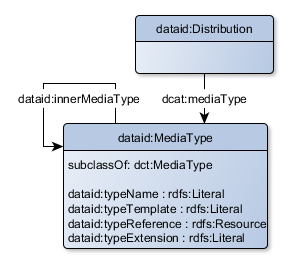
\includegraphics[width=7cm]{images/ClassMediaType.png}
  \caption{The MediaType concept.}
  \label{fig:example}
\end{figure}

The following extract exemplifies the use of these properties:
\footnote{note: the namespace \url{http://dataid.dbpedia.org/ns/mt#} for common MediaTypes is used on a preliminary basis)}
\\
\begin{lstlisting}[language=ttl, captionpos=b,caption=Example of a complex MediaType,label=lst:coresuperset,linewidth=\columnwidth,breaklines=true]
<http://dataid.dbpedia.org/ns/mt#MediaType_turtle_x-bzip2>
        a                      dataid:MediaType ;
        dataid:innerMediaType  <http://dataid.dbpedia.org/ns/mt#MediaType_turtle> ;  
        dataid:typeName        "Turtle Bzip2" ;
        dataid:typeExtension   ".bz2" ;  
        dataid:typeTemplate    "application/x-bzip2" 

<http://dataid.dbpedia.org/ns/mt#MediaType_turtle>
        a                     dataid:MediaType ;
        dataid:typeName       "Turtle" ;
        dataid:typeExtension  ".ttl" ;
        dataid:typeTemplate   "application/x-turtle" ;   
        dataid:typeTemplate   "text/turtle" .
\end{lstlisting}

\subsection{Agent} 
\label{sec:coreagent}
An \important{Agent} is something or someone that bears some form of responsibility for an \important{Entity} or activities which create, transform or manage \important{Entities} in some way. \important{Agents} are real or legal persons, groups of persons, programs, organisations, etc. The class \prop{dataid:Agent} subsumes both agent concepts of the \prov and \foaf ontologies, to further incorporate \prov into the context of \dcat (which uses the class \prop{foaf:Agent} to portray this concept). 

The attributes of the \foaf vocabulary\footnoteurl{http://xmlns.com/foaf/spec/} are used to describe aspects such as name and e-mail address of a person. In addition, the following properties were introduced in \core:

\begin{description}
\item[\prop{dataid:hasAuthorization}:] the inverse property of \prop{dataid:authorizedAgent}, pointing out an \important{Authorization} which grants an \important{Agent} some kind of authority over \important{Entities}. This is explained in detail in the example on \important{Authorizations} in the next \Cref{sec:coreauthorization}. \hfill\textbf{(R)}
\item[\prop{dataid:identifier}:] often, \important{Agents} already have unique identifiers specified in a different context on the Web (in addition to the URI used in the context of a \dataid document, such as URI, ORCID\footnoteurl{http://orcid.org} or researcherId\footnoteurl{http://www.researcherid.com}). This property points out additional identifiers (cf. \Cref{sec:coreidentifier}). \hfill\textbf{(O)}
\end{description}

\begin{figure}[!htbp]
\centering
  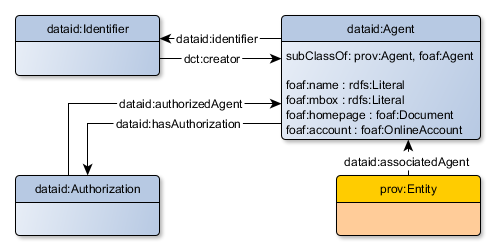
\includegraphics[width=12cm]{images/ClassAgent.png}
  \caption{The Agent concept}
  \label{fig:example}
\end{figure}

\pagebreak
This example of an \important{Agent} portrays the \dbpedia Association\footnoteurl{http://wiki.dbpedia.org/dbpedia-association}:
\\
\begin{lstlisting}[language=ttl, captionpos=b,caption=Example of an Agent,label=lst:coresuperset,linewidth=\columnwidth,breaklines=true]
<http://wiki.dbpedia.org/dbpedia-association>
        a                        dataid:Agent ;
        dataid:hasAuthorization  <dataid_ar.ttl?auth=creatorAuthorization> ; 
        foaf:homepage            <http://dbpedia.org> ;
        foaf:mbox                "dbpedia@infai.org" ;                                                        
        foaf:name                "DBpedia Association" .
\end{lstlisting}

\subsection{Authorization} 
\label{sec:coreauthorization}
One objective of \core is the detailed expression of the relations between \important{Agents} and \important{Entities}. To qualify these relations (summarised under the property \prop{dataid:associatedAgent}) \important{AgentRoles} have to be assigned to the involved \important{Agents} (such as \important{Maintainer}, \important{Publisher}, etc.). This is achieved by the class \prop{dataid:Authorization}, which is a sub-class of \prop{prov:Attribution}, a qualification of the property \prop{prov:wasAttributedTo}. It basically states, which \important{AgentRoles} (pointed out with \prop{dataid:authorityAgentRole}) an \important{Agent} (via \prop{dataid:authorizedAgent}) has, regarding a certain collection of \important{Entities} (\prop{dataid:authorizedFor}). This mediator is further qualified by an optional period for which it is valid and access restrictions by the \important{Entities} themselves, allowing only specific \important{Authorizations} to exert influence over them (cf. \prop{dataid:needsSpecialAuthorization}). 

\Cref{sec:exauthorization} contains a detailed example on \important{Authorizations}, to deepen the understanding of this concept as well as to provide a suitable use case.

\begin{figure}[!htbp]
\centering
  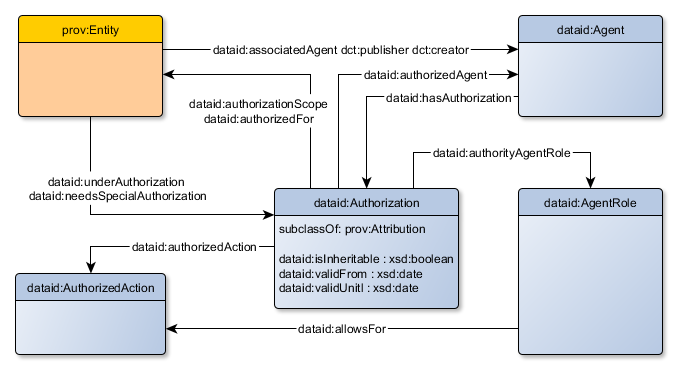
\includegraphics[width=\textwidth]{images/ClassAuthorization.png}
  \caption{The Authorization concept}
  \label{fig:example}
\end{figure}

\begin{description}
\item[\prop{dataid:authorizedAgent}:] each \important{Authorization} shall have at least one associated \important{Agent}, which is pointed out via this property (sub-property of \prop{prov:agent}). \hfill\textbf{(M)}
\item[\prop{dataid:authorityAgentRole}:] provides the \important{AgentRole} the \important{Agent}(s) of this \important{Authorization} are assigned with (sub-property of \prop{prov:hadRole}). \hfill\textbf{(M)}
\item[\prop{dataid:authorizedFor}:] points out those \important{Entities} for which this \important{Authorization} is valid (sub-property of \prop{dataid:authorizationScope}). \hfill\textbf{(M)}
\item[\prop{dataid:authorizedAction}:] an \important{AgentRole} entails the right (or responsibility) for \important{Agents} to execute a predefined collection \important{AuthorizedAction}(s). This property can be inferred by a chain of properties (OWL property chain axiom): \prop{dataid:authorityAgentRole} / \prop{dataid:allowsFor}. \hfill\textbf{(O)}
\item[\prop{dataid:isInheritable}:] indicates whether an \important{Authorization} is transferable when changing versions of a \dataid. Thus, keeping \important{Agent}, \important{AgentRole} and \important{Actions} in place for the updated versions of all involved \important{Entities}. \textbf{(O)}
\item[\prop{dataid:validFrom}:] defining the temporal beginning (inclusive) of an \important{Authorization} (the time from which on out the axioms of an \important{Authorization} are valid). \hfill\textbf{(O)}
\item[\prop{dataid:validUntil}:] defining the temporal ending (exclusive) of an \important{Authorization} (the time from which on out the axioms of an \important{Authorization} are no longer valid). \hfill\textbf{(O)}
\end{description}

The property \prop{dataid:authorizationScope} is an abstract super-property of \prop{dataid:authorizedFor}, pointing to all referred and inferred \important{Entities} which are under a certain \important{Authorization}. Triples with this predicate are inferred by its sub-properties \prop{dataid:authorizedFor} and the virtual properties \prop{dataid:authorizationChain1} to \prop{dataid:authorizationChain9}. 

Furthermore, property \prop{dataid:underAuthorization} is the inverse of \prop{dataid:authorizationScope} and a sub-property of \prop{prov:wasAttributedTo}. It points out an \important{Authorization} which qualifies the relation \prop{dataid:associatedAgent} of an \important{Entity}. Its sub-property \prop{dataid:needsSpecialAuthorization} was introduced to restrict the reach of \important{Authorizations}, to the exclusion of those \important{Authorizations}, not referenced via this property (or simply: if an \important{Entity} has a \prop{dataid:needsSpecialAuthorization} instance, all \important{Authorizations} without this referral have no influence over this \important{Entity}, disregarding its specification). An exact explanation of \important{Authorizations} and all involved properties is accompanying the extended example on \important{Authorizations} at the end of this chapter (cf. \Cref{sec:exauthorization}).

The following snippet provides a simple example of two \important{AgentRoles} being assigned to two \important{Agents} for a \important{DataId} instance (and thereby for every \important{Entity} involved in this \dataid  - see \Cref{sec:exauthorization} for more).
\\
\begin{lstlisting}[language=ttl, captionpos=b,caption=Example of two Agents and their pertaining Authorizations,label=lst:coresuperset,linewidth=\columnwidth,breaklines=true]
<http://wiki.dbpedia.org/dbpedia-association/persons/Freudenberg>
        a                        dataid:Agent ;                                               
        dataid:hasAuthorization  <dataid_ar.ttl?auth=maintainerAuthorization> ;
        foaf:mbox                "freudenberg@informatik.uni-leipzig.de" ;
        foaf:name                "Markus Freudenberg"                     ;
        dataid:identifier        <http://www.researcherid.com/rid/L-2180-2016> .              

<dataid_ar.ttl?auth=maintainerAuthorization>
        a                          dataid:Authorization ;                                     
        dataid:authorityAgentRole  dataid:Maintainer ;                                        
        dataid:authorizedAgent     <http://wiki.dbpedia.org/dbpedia-association/persons/Freudenberg> ;
        dataid:authorizedFor       <dataid_ar.ttl> .                                          

<http://wiki.dbpedia.org/dbpedia-association>
        a                        dataid:Agent ;                                               
        dataid:hasAuthorization  <dataid_ar.ttl?auth=creatorAuthorization> ;
        foaf:homepage            <http://dbpedia.org> ;
        foaf:mbox                "dbpedia@infai.org" ;
        foaf:name                "DBpedia Association" .

<dataid_ar.ttl?auth=creatorAuthorization>
        a                          dataid:Authorization ;
        dataid:authorityAgentRole  dataid:Creator ;                                           
        dataid:authorizedAgent     <http://wiki.dbpedia.org/dbpedia-association> ;
        dataid:authorizedFor       <dataid_ar.ttl> .
\end{lstlisting}

\subsection{AuthorizedAction \& AgentRole} 
\label{sec:coreaction}
The \important{AgentRole} assigned to an \important{Agent} in the context of an \prop{dataid:Authorization} is defined only by the property \prop{dataid:allowsFor}, pointing out the \important{AuthorizedActions} it entails. A \prop{dataid:AuthorizedAction} shall either be a \prop{dataid:EntitledAction}, representing all \important{AuthorizedActions} an \important{Agent} could take, or the \important{AuthorizedActions} an \important{Agent} has to take (\prop{dataid:ResponsibleAction}). 

\begin{figure}[!htbp]
\centering
  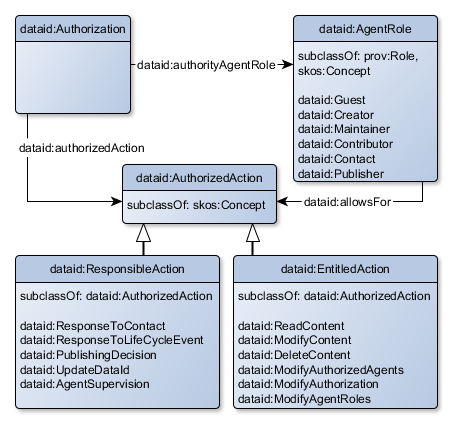
\includegraphics[width=9cm]{images/ClassAuthorizedAction.png}
  \caption{The AuthorizedAction and AgentRole concepts}
  \label{fig:example}
\end{figure}

\important{AuthorizedActions} and \important{AgentRoles} defined in this ontology are only examples of possible implementations, reflecting a common environment of a File or Document Management System. They can be replaced to fit the use case at hand. Implementing them as a \prop{skos:ConceptScheme}\footnoteurl{https://www.w3.org/TR/skos-reference/#ConceptScheme} offers additional semantics, for example in determining which \important{AgentRole} can override \important{AuthorizedActions} initiated by \important{Agents} with other \important{AgentRoles} for the same \important{Entity}. The following descriptions will shortly introduce each individual of these classes, predefined in the \core ontology.

{\large\textbf{AgentRoles:}}
\begin{description}
\item[\prop{dataid:Creator}:] Creator of the resource. An \important{AgentRole} that is credited with the main part in the initial creation of the resource.
\item[\prop{dataid:Contact}:] An \important{Agent} that can be contacted for general requests about the resource.
\item[\prop{dataid:Contributor}:] Contributor to the resource. An \important{Agent} that was involved in creating or maintaining the resource but did not have the main part in this activity.
\item[\prop{dataid:Guest}:] A visitor or anonymous \important{Agent} which only has the right to read public documents.
\item[\prop{dataid:Maintainer}:] Maintainer of the \important{Dataset}. An \important{Agent} that ensures the technical correctness, accessibility and up-to-dateness of a \important{Dataset}.
\item[\prop{dataid:Publisher}:] An \important{Agent} that makes the \important{Dataset} accessible online on a server or repository without necessarily being involved in its creation and decides on all dissemination related tasks as well (e.g. data portal entries).
\\
\end{description}

{\large\textbf{ResponsibleActions:}}
\begin{description}
\item[\prop{dataid:ResponseToContact}:] The responsibility to respond to contact attempts by external \important{Agents}. A contact point for the \important{Entity}.
\item[\prop{dataid:ResponseToLifeCycleEvent}:] The responsibility to manage changes and react to any event related to the lifecycle of a \important{Dataset} (e.g. issue tracker entries, unavailable download URL, etc.).
\item[\prop{dataid:PublishingDecision}:] The final decision if an \important{Entity} (or a version of it) should be published.
\item[\prop{dataid:UpdateDataId}:] The responsibility to update dataset metadata.
\item[\prop{dataid:AgentSupervision}:] The responsibility to supervise other \important{Agents}.\\
\end{description}

{\large\textbf{EntitledActions:}}
\begin{description}
\item[\prop{dataid:ReadDataId}:] read the \dataid dataset metadata.
\item[\prop{dataid:ReadContent}:] read the content of an \important{Entity}.
\item[\prop{dataid:ModifyContent}:] modify the content of an \important{Entity}.
\item[\prop{dataid:DeleteContent}:] delete some content of an \important{Entity}.
\item[\prop{dataid:ModifyAuthorization}:] modify an \important{Authorization}.
\item[\prop{dataid:ModifyAgentRoles}:] modify \important{AgentRoles} and \important{AuthorizedActions}.
\end{description}

This example has been lent from the \core ontology document itself. Here the \important{AgentRole} 'Contact' is defined in the context of a \prop{skos:ConceptScheme}.
\\
\begin{lstlisting}[language=ttl, captionpos=b,caption=Example of an AgentRole definition,label=lst:coresuperset,linewidth=\columnwidth,breaklines=true]
dataid:Contact
	a owl:NamedIndividual, dataid:AgentRole;
	rdfs:isDefinedBy <http://dataid.dbpedia.org/ns/core#> ;
	dataid:allowsFor dataid:ReadDataId; 
	dataid:allowsFor dataid:ModifyContent;
	dataid:allowsFor dataid:ReadContent;
	dataid:allowsFor dataid:ResponseToContact;
        rdfs:comment "An agent that can be contacted for general requests about the resource."@en ;
        skos:prefLabel "contact"@en ;
	skos:inScheme dataid:AgentRoleScheme ; 
	skos:broader dataid:Publisher, dataid:Maintainer .   
\end{lstlisting}

\subsection{DatasetRelationship} 
\label{sec:corerelation}
A \important{DatasetRelationship} is a qualification of the generic property \prop{dataid:relatedDataset} (which is a sub-property of \prop{dct:relation}). The \prop{dataid:DatasetRelationship} is a subclass of \prop{prov:EntityInfluence} and is defined by three properties:

\begin{description}
\item[\prop{dataid:datasetRelationRole}:] specifying the role (or type) of this relationship, defining the exact role the 'target' \important{Dataset} takes regarding the 'origin' \important{Dataset} of this relationship. \hfill\textbf{(M)}
\item[\prop{dataid:qualifiedRelationOf}:] the inverse property of \prop{dataid:qualifiedDatasetRelation} is pointing out the origin \important{Dataset} of this qualification. \hfill\textbf{(M)}
\item[\prop{dataid:qualifiedRelationTo}:] the target \important{Dataset} of this qualification. \hfill\textbf{(M)}
\end{description}

\begin{figure}[!htbp]
\centering
  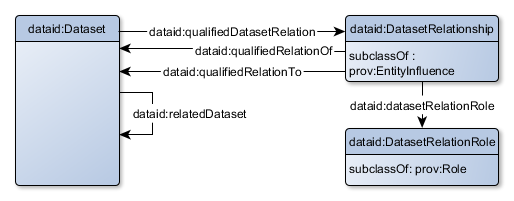
\includegraphics[width=12cm]{images/ClassDatasetRelationship.png}
  \caption{The DatasetRelationship and DatasetRelationRole concept}
  \label{fig:example}
\end{figure}

The class \prop{dataid:DatasetRelationRole} is not further qualified in the context of \core, which could be done in an extension to \core, similar to \prop{dataid:AgentRole}. Some instances of this class are already provided:

\begin{description}
\item[\prop{dataid:GenericRelation}:] specifies a \prop{dataid:DatasetRelationship} between two \important{Datasets} which have a relation to an unknown quality (such a relation is equivalent to direct \prop{dct:relation} property).
\item[\prop{dataid:DerivateRole}:] specifies a \prop{dataid:DatasetRelationship} where one \important{Dataset} points out a second \important{Dataset}, which is a derivate of the first.
\item[\prop{dataid:SourceRole}:] specifies a \prop{dataid:DatasetRelationship} where the origin \important{Dataset} is created by transforming/collecting data from the target \important{Dataset}.
\item[\prop{dataid:CopyRole}:] specifies a \prop{dataid:DatasetRelationship} where the origin \important{Dataset} is an exact copy of the target \important{Dataset} (e.g. when republished under a different domain).
\item[\prop{dataid:SimilarityRole}:] specifies a \prop{dataid:DatasetRelationship} where the origin \important{Dataset} has a significant similarity to the target \important{Dataset} (without any assertion as to a dimension of similarity).
\end{description}

In the example, the \wikipedia source Dataset (named 'pages\_articles') of a given \dbpedia dataset is referred to with the help of this concept:
\\
\begin{lstlisting}[language=ttl, captionpos=b,caption=Example of a DatasetRelationship,label=lst:coresuperset,linewidth=\columnwidth,breaklines=true]
<dataid_ar.ttl?relation=source&target=pages_articles>
        a                           dataid:DatasetRelationship ;
        dataid:datasetRelationRole  dataid:SourceRole ;
        dataid:qualifiedRelationOf  <dataid_ar.ttl?set=long_abstracts_en_uris> ;
        dataid:qualifiedRelationTo  <dataid_ar.ttl?set=pages_articles> .  
\end{lstlisting}

\subsection{Identifier} 
\label{sec:coreidentifier}
The class \prop{dataid:Identifier} uniquely identifies any resource (incl. \important{Entities} and \important{Agents}), given an identifier as a literal and a corresponding \prop{datacite:IdentifierScheme} (e.g. ORCID, ResearcherID etc.). Typically an organisation is responsible for issuing and managing Identifiers described with this concept, which can be referred to with \prop{dct:creator}. \core adopted this approach from Datacite ontology (cf. \Cref{sec:datacite}) to provide a schematic way of adding additional, existing identifiers to \important{Entities} and \important{Agents} referenced in a \dataid document.

\begin{figure}[!htbp]
\centering
  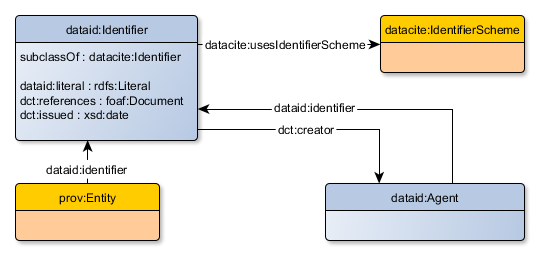
\includegraphics[width=12cm]{images/ClassIdentifier.png}
  \caption{The Identifier concept}
  \label{fig:example}
\end{figure}

\pagebreak
\begin{description}
\item[\prop{dataid:literal}:] the identifier as literal (e.g. a URI as literal). \hfill\textbf{(M)}
\item[\prop{datacite:usesIdentifierScheme}:] an IdentifierScheme defines (among other attributes) a pattern against which the literal of an identifier is validated. Thereby the validity of an identifier is tested. \hfill\textbf{(M)}
\item[\prop{dct:references}:] often identifier agencies have web presentations for their identifiers (e.g. ORCID\footnoteurl{http://orcid.org/0000-0002-1825-0097}). Such a website can be referenced with this property. \hfill\textbf{(O)}
\item[\prop{dct:creator}:] can be used to identify the identifier agency, responsible for an identifier and pertaining scheme. \hfill\textbf{(O)}
\\
\end{description}

\begin{lstlisting}[language=ttl, captionpos=b,caption=Example of an Identifier,label=lst:coresuperset,linewidth=\columnwidth,breaklines=true]
<http://www.researcherid.com/rid/L-2180-2016>
        a                              dataid:Identifier ;
        dataid:literal                 "L-2180-2016" ;                                        
        dct:issued                     "2016-08-01"^^xsd:date ;
        dct:references                 <http://www.researcherid.com/rid/L-2180-2016> ;        
        datacite:usesIdentifierScheme  datacite:researcherid .  
\end{lstlisting}

\subsection{SimpleStatement} 
\label{sec:corestatement}
The concept \prop{dataid:SimpleStatement} is intended as a tool for conveying a statement, definition or point of view about a certain topic. Using either a simple literal (\prop{dataid:literal}) to provide a quotation or by a referencing a web resource providing or representing the statement in any medium (picture, text, video, etc.). This class is a sub-class of \prop{prov:Entity} and implements also the following Dublin Core classes: \prop{dct:ProvenanceStatement}, 
\prop{dct:RightsStatement},
\prop{dct:Standard}
. With this measure, it is possible to attach provenance information onto instances of this concept and to use \prop{dataid:SimpleStatement} as the range of \prop{dct:rights} and its sub-properties, \prop{dct:provenance}, \prop{dct:conformsTo} and others.

This reification approach with an intermediate resource was chosen to cover as many scenarios as possible including many edge cases which do not have to be modelled explicitly. To provide a minimum of structure for textual statements, as well as providing a resource onto which provenance information could be attached.

\begin{figure}[!htbp]
\centering
  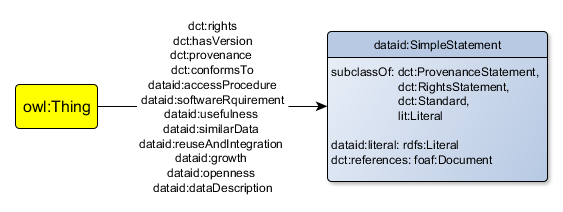
\includegraphics[width=12cm]{images/ClassSimpleStatement.png}
  \caption{The SimpleStatement concept}
  \label{fig:example}
\end{figure}

\pagebreak
\begin{description}
\item[\prop{dataid:literal}:] a textual statement 'from humans for humans'. \hfill\textbf{(R)}
\item[\prop{dct:references}:] the alternative reference to a web resource containing the  statement comprehensible by humans. \hfill\textbf{(O)}
\end{description}

Two instances from the running example demonstrating the different usage scenarios of this concept. The first is the official rights statement of the \dbpedia Association, while the second is the access procedure for the \dbpedia SPARQL endpoint, where \prop{dct:reference} is pointing out the SPARQL 1.1 specification (as a web page specifying the means of querying the endpoint).
\\
\begin{lstlisting}[language=ttl, captionpos=b,caption=Examples of SimpleStatements,label=lst:coresuperset,linewidth=\columnwidth,breaklines=true]
<dataid_ar.ttl?rights=dbpedia-rights>
        a                 dataid:SimpleStatement ;                                            
        dataid:literal  """DBpedia is derived from Wikipedia and is distributed under the same licensing terms as Wikipedia itself. As Wikipedia has moved to dual-licensing, we also dual-license DBpedia starting with release 3.4. Data comprising DBpedia release 3.4 and subsequent releases is licensed under the terms of the Creative Commons Attribution-ShareAlike 3.0 license and the GNU Free Documentation License. Data comprising DBpedia releases up to and including release 3.3 is licensed only under the terms of the GNU Free Documentation License."""@en .

<dataid_ar.ttl?stmt=sparqlaccproc>
        a                 dataid:SimpleStatement ;                                            
        dct:references    <https://www.w3.org/TR/sparql11-overview/> ;                        
        dataid:literal  "An endpoint for sparql queries: provide valid queries."@en .
\end{lstlisting}

\pagebreak
\section{Complex Example on Authorizations} 
\label{sec:exauthorization}

I decided to provide a more prolific example on the subject of \important{Authorizations} since this concept is of more complex nature. In particular, the impact of \prop{dataid:authorizationScope} with its sub-properties is difficult to understand at first sight.

The property \prop{dataid:authorizationScope} has the role of an abstract super property, pointing out all referred and inferred \important{Entities} under a given \important{Authorization} and is usually not instantiated in a \dataid graph. It can be inferred directly by the existence of property \prop{dataid:authorizedFor}, which is used to reference \important{Entities} to which an \important{Authorization} applies and its rules and restrictions are tailored for.

The following axioms for the transitive property \prop{dataid:authorizationScope} would be desirable to extend the influence of an \important{Authorization} along any property path combined of \prop{foaf:primaryTopic}, \prop{void:subset} and \prop{dcat:distribution}, initiated by an instance of \prop{dataid:authorizedFor}.

{\footnotesize
\vspace*{-0.5cm}
\begin{align*}
foaf:primaryTopic \sqsubseteq dataid:authorizationScope\\
void:subset \sqsubseteq dataid:authorizationScope\\
dcat:distribution \sqsubseteq dataid:authorizationScope\\
dataid:authorizedFor \sqsubseteq dataid:authorizationScope
\end{align*}
}%
To not hijack foreign ontologies \cite{feeney2015linked} (i.e. \dcat, \void or \foaf), a series of properties (\prop{dataid:authorisationChain1} - \prop{dataid:authorisationChain9}) were introduced to simulate this behaviour with the help of the OWL property chain axiom\footnoteurl{https://www.w3.org/TR/owl-primer/#Property_Chains}.

Properties \prop{dataid:authorisationChain1} to \prop{dataid:authorisationChain6}:

{\footnotesize
\vspace*{-0.5cm}
\begin{align*}
foaf:primaryTopic \circ dcat:distribution \sqsubseteq dataid:authorizationScope\\
foaf:primaryTopic \circ void:subset \sqsubseteq dataid:authorizationScope\\
void:subset \circ dcat:distribution \sqsubseteq dataid:authorizationScope\\
void:subset \circ void:subset \sqsubseteq dataid:authorizationScope\\
void:subset \circ void:subset \circ dcat:distribution \sqsubseteq dataid:authorizationScope\\
foaf:primaryTopic \circ void:subset \circ dcat:distribution \sqsubseteq dataid:authorizationScope
\end{align*}
}%
With these properties, all subsequent \important{Entities} connected to the origin \important{Entity} (the \important{Entity} referenced from an \important{Authorization} with \prop{dataid:authorizedFor}), are under the influence of this \important{Authorization}, connected with it via the transitive property \prop{dataid:authorizationScope}. One exception remains: those \important{Entities} second in line after the origin \important{Entity} are skipped in this progression.
Properties \prop{dataid:authorisationChain7} to \prop{dataid:authorisationChain9} are solving this issue:

{\footnotesize
\vspace*{-0.5cm}
\begin{align*}
dataid:authorizedFor \circ foaf:primaryTopic \sqsubseteq dataid:authorizationScope\\
dataid:authorizedFor \circ void:subset \sqsubseteq dataid:authorizationScope\\
dataid:authorizedFor \circ dcat:distribution \sqsubseteq dataid:authorizationScope
\end{align*}
}%
For example: if a knowledge base (KB) holds some statements, such as:
\begin{lstlisting}[language=ttl, captionpos=b,label=lst:coresuperset,linewidth=\columnwidth,breaklines=true]
ex:someAuthorization	dataid:authorizedFor		ex:DataId .
ex:DataId		foaf:primaryTopic		ex:RootDataset .
ex:RootDataset		void:subset			ex:DatasetC . 
\end{lstlisting}

we can infer the following statements:
\begin{lstlisting}[language=ttl, captionpos=b,label=lst:coresuperset,linewidth=\columnwidth,breaklines=true]
ex:someAuthorization 	dataid:authorizationScope 	ex:DataId .
ex:someAuthorization 	dataid:authorizationScope 	ex:RootDataset .
ex:someAuthorization 	dataid:authorizationScope 	ex:DatasetC . 
\end{lstlisting}

by inferring these statements first:	
\begin{lstlisting}[language=ttl, captionpos=b,label=lst:coresuperset,linewidth=\columnwidth,breaklines=true]
ex:DataId 		dataid:authorizationChain2 	ex:DatasetC .
ex:someAuthorization 	dataid:authorizationChain7 	ex:RootDataset .
\end{lstlisting}

With these virtual properties the inference of \prop{dataid:authorizationScope} along the depicted property paths becomes feasible:

\begin{figure}[!htbp]
\vspace*{-0.5cm}
\centering
  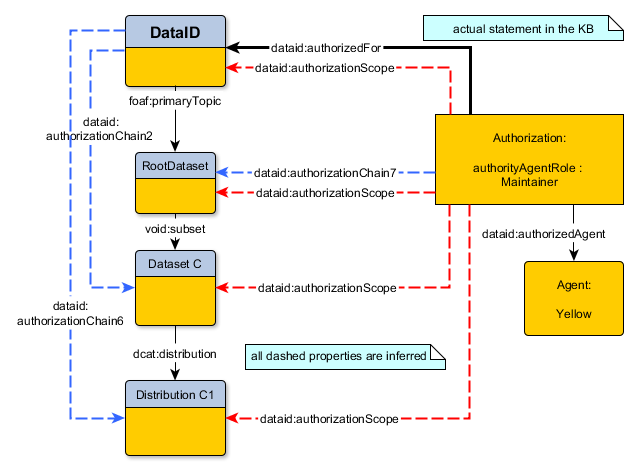
\includegraphics[width=12cm]{images/AuthorizationExample.png}
  \caption{Inferences of \prop{dataid:authorizationScope}}
  \label{fig:dlaxioms}
\end{figure}

Here the \important{Authorization} for \important{Agent} Yellow is not only valid for the \important{DataId} entity, referred to via \prop{dataid:authorizedFor}. By inferring additional statements of this kind, the scope of this \important{Authorization} is extended to every \important{Dataset} and \important{Distribution} connected via \prop{foaf:primaryTopic}, \prop{dcat:distribution} and \prop{void:subset}. By this means, extending the influence (or scope) of an \important{Authorization} over multiple \important{Entities}, without having to point out all of them with \prop{dataid:authorizedFor}, is realised. External properties involved did not have to be distorted, by adding sub-property axioms or an inclusion of rule-based axioms (such as SWRL\footnoteurl{https://www.w3.org/Submission/SWRL/}), avoiding unforeseeable complications in use case extensions, importing \core.

The automatic extension of an \important{Authorization} has also its drawbacks. By introducing multiple \important{Authorizations} in the context of a \dataid document, providing the same \important{AgentRole} for an \important{Entity}, the author can encounter unintended behaviours. In this example the previous context is enriched by introducing an additional \important{Agent} Blue with \important{AgentRole} \important{Maintainer}:

\begin{figure}[!htbp]
\centering
  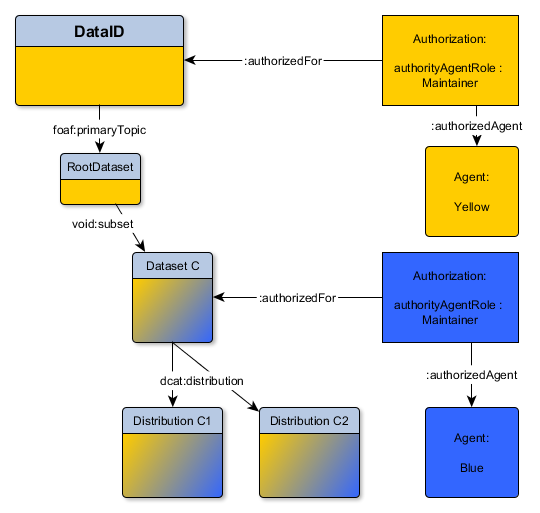
\includegraphics[width=10cm]{images/AuthorizationExample2.png}
  \caption{Two Agents sharing responsibilities of a Maintainer}
  \label{fig:dlaxioms}
\end{figure}

\textit{Dataset C} (and all its \important{Distributions}) has two \important{Maintainers}, both equally permitted to wield \important{AuthorizedActions} as defined by the definition of \prop{dataid:Maintainer}. This behaviour may or may not be intended by the author. To provide the means for restricting \important{Entities} to specific \important{Authorizations}, the property \prop{dataid:needsSpecialAuthorization} was introduced. This sub-property of \prop{dataid:underAuthorization} (the inverse of \prop{dataid:authorizationScope}) allows to point out those \important{Authorizations} with sufficient importance to exert their authority over an \important{Entity}, to the exclusion of other \important{Authorizations} referenced via \prop{dataid:authorizationScope}.

The following example again expands the already known scenario, by introducing a third \important{Authorization} for \important{Agent} Green:

\begin{figure}[!htbp]
\centering
  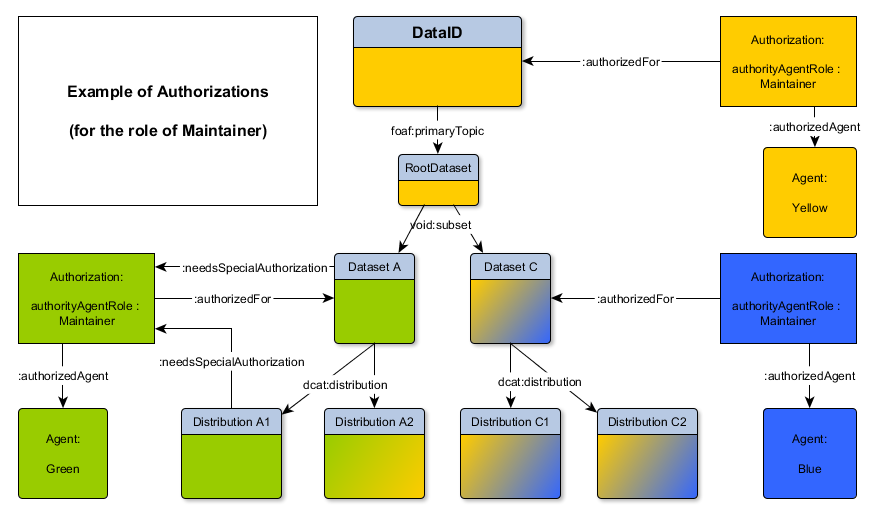
\includegraphics[width=\textwidth]{images/AuthorizationExample5.png}
  \caption{Restricting the influence of Authorizations}
  \label{fig:dlaxioms}
\end{figure}

While \textit{Dataset A} and \textit{Distributions A1} and \textit{A2} are under the \important{Authorizations} of \important{Agent} Yellow and \important{Agent} Green, only \textit{Distribution A2} will be maintained by both \important{Agents}. \textit{Dataset A} and \textit{Distribution A1} require specifically the \important{Authorization} of \important{Agent} Green for the purpose of providing the \important{AgentRole} of \important{Maintainer}.

This mechanism is useful when introducing different levels of privacy into the domain, for example, a Document Management System (DMS). Two groups of users are specified: The first group (yellow group) should only be able to read the content of a given collection of documents, while the second group (blue group) is also allowed to modify these documents. Therefore, defining two new \important{AgentRoles} is advisable. \important{AgentRole} 'Reader' can only read the content of \important{Entities} available to it, while the 'Editor' also allows for modifying the content. These \important{AgentRoles} are linked to via \prop{dataid:authorityAgentRole} from the respective \important{Authorizations} of the two groups (\prop{dataid:authorizedAgent} points out the members of a group).

\begin{figure}[!htbp]
\centering
  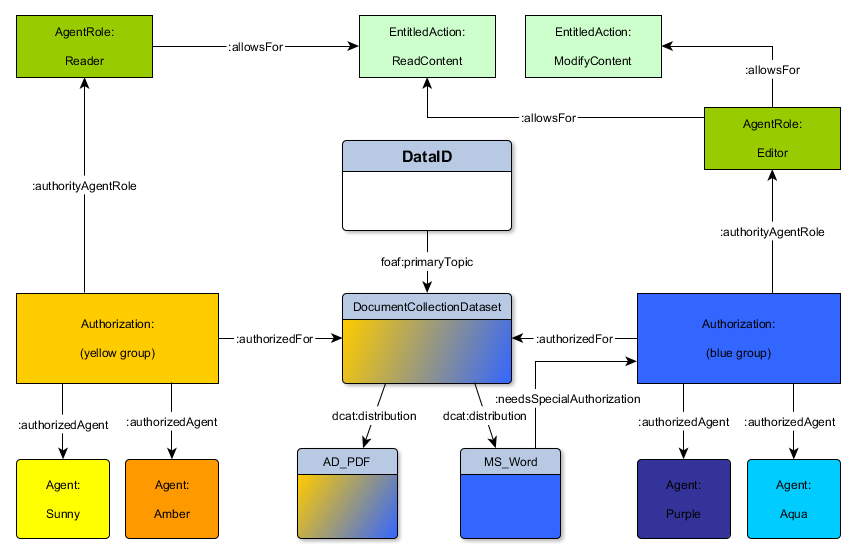
\includegraphics[width=\textwidth]{images/DmsExample.png}
  \caption{Example: Document Management System}
  \label{fig:dlaxioms}
\end{figure}

Both \important{Authorizations} are authorised for the same document collection (\important{Dataset}) and its \important{Distributions} as PDF and MS\_Word versions of the same content in the DMS. Since the MS\_Word version of the documents is used for editing the content, while its PDF counterpart is the publishing version, it is sensible to allow only the Editors (blue group) access to the MS\_Word \important{Distribution} by using \prop{dataid:needsSpecialAuthorization}. 

\chapter{Publishing Datasets with DataID}
\label{chap:bestprctice}

\section{Best Practices} 
\label{sec:bestprctice}
Best practices on any kind of methodology or problem have become a ubiquitous presence in the current landscape of the World Wide Web. Be it a Ted Talk on how to live to be 100\footnoteurl{https://www.ted.com/talks/dan_buettner_how_to_live_to_be_100} or how to get accurate results when using machine learning techniques\footnoteurl{http://machinelearningmastery.com/machine-learning-checklist/}.

Astonishingly, when it comes to publishing data in a widely accepted manner, only a hand full of comprehensive best practices exist. Most of these best practices, workflows or checklists are further constricted to a certain field of research, methodology or data type:

\begin{description}
\item[Methodological Guidelines for Publishing
Government Linked Data] "[...] a preliminary set of methodological guidelines for generating, publishing and exploiting Linked Government Data" \cite{Terrazas}
\item[Best Practices for Publishing Linked Data] "[...] a series of best practices designed to facilitate development and delivery of open government data as Linked Open Data." \cite{Hyland:14:BPP}
\item[Key components of data publishing] "From an assessment of the current data-publishing landscape, we highlight important gaps and challenges to consider, especially when dealing with more complex workflows and their integration into wider community frameworks." \cite{austin_2015_34542}
\item[]
\end{description}
There are two not quiet distinct categories of best practices on data publishing: workflows and checklists. 

\paragraph{Workflows} introduce a specific order of activities, the flow of artefacts between them as well as agents and their roles in these processes. Workflows are often summarised in so called Data Lifecycles (or Data Engineering Lifecycle).

The LOD2 Lifeycle of Linked Data \cite{AuerBDEHILMMNSTW12} - used by the ALIGNED project (cf. \Cref{fig:aligned}) - is a portrayal of such a workflow in a domain-specific environment.

\begin{figure}[!htbp]
\centering
  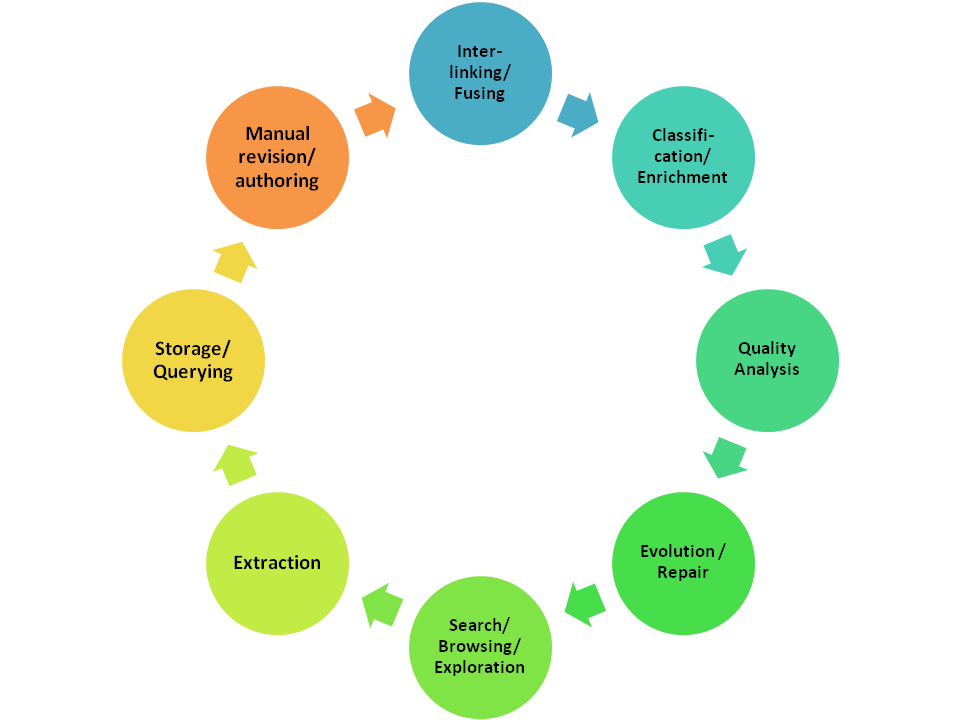
\includegraphics[width=12cm]{images/lod2lifecycle.png}
  \caption{The LOD2 Lifecycle of Linked Data \cite{AuerBDEHILMMNSTW12}}
  \label{fig:lod2lifecycle}
\end{figure}

Many depictions of Data Engineering Lifecycles have domain-independent similarities.
Villaz\'{o}n-Terrazas et al. presented a more generic version of such a cycle, which I am going to adopt in the context of this work.

 \begin{figure}[!htbp]
\centering
  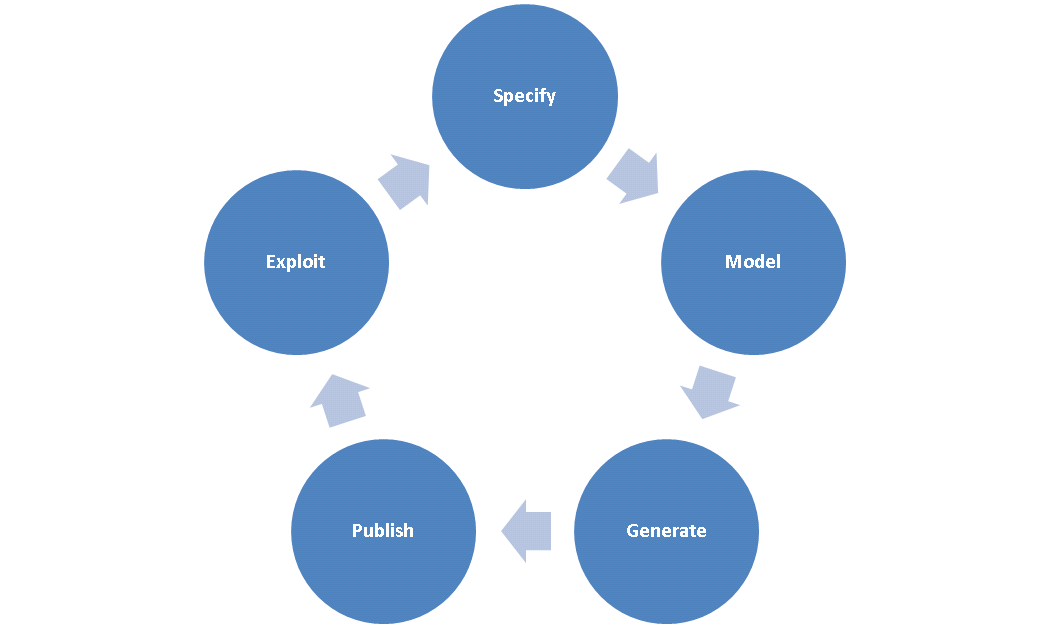
\includegraphics[width=11cm]{images/Villazon-terrazas.png}
  \caption{The Government Linked Data Lifecycle \cite{Terrazas}}
  \label{fig:gldlifecycle}
\end{figure}

A concise summary, tracing the bubble graph above:

\begin{itemize}
\item Specify
\begin{itemize}
\item analysis of data sources (what data is useful) or previous version of the dataset
\item Select/Design an identifier scheme used to identify all instances
\item decide on data type and serialisation of you data
\end{itemize}
\item Model
\begin{itemize}
\item search/create/update a suitable schema/vocabulary on which to base the datasets
\end{itemize}
\item Generate
\begin{itemize}
\item transform the data sources
\item clean (and validate) the result
\end{itemize}
\item Publish
\begin{itemize}
\item improve discoverability (choose suitable data portal, announce release at different venues)
\item publish the created datasets
\item publish the pertaining metadata
\end{itemize}
\item Exploit
\begin{itemize}
\item different consumer side activities (browsing, integrating, analysing etc.)
\item collect feedback from consumers, improve data
\end{itemize}
\end{itemize}

\paragraph{Checklists} are collections of general advises, how-tos and precautions on publishing data without a particular order of items. 

The most comprehensive collection of best practices about publishing data has emerged with the establishment  
of the 'Data on the Web' W3C working group\footnoteurl{https://www.w3.org/2013/dwbp/wiki/Main_Page} and their best practices document \cite{dwbpW3C2016} (released as recommendation candidate by the time of writing). 

%Besides the set of best practices, a list of benefits for publishing data on the Web is presented in this document

This set of recommendations touches upon most of the crucial issues when publishing data (with the noted exception of dissemination tasks). I endorse these 35 best practices to their full extent and recommend to follow all of the suggestions made. Datasets conform to these suggestions, would reap all benefits towards which these practices were created: \textit{Reuse, Comprehention, Linkability, Discoverabilty, Trust, Access, Interoperability and Processability} \cite{dwbpW3C2016}.

A different selection of best practices was already discussed in \Cref{sec:fair}. The FAIR principles \cite{fair2016} are ensuring the quality of data concerning machine-readability, discovery and reuse. 

In this chapter, I want to build on these foundations, by expanding on metadata composition and deployment with \dataid (\Cref{sec:composingmetadata}). In addition, I want to contribute to the discussion on publishing data. A checklist for publishing Linked Data datasets is presented in \Cref{sec:checklist}, based on the experiences accumulated from publishing official \dbpedia releases.

\section{Composing and Publishing DataID based Metadata} 
\label{sec:composingmetadata}
The data engineering lifecycle depicted in \Cref{fig:gldlifecycle} does not only apply to the data being generated and published. It is also a valid depiction of a lifecycle for metadata which is co-evolving parallel to the data it is portraying.

In the case of \dataid metadata, the tasks necessary to eventually publish a metadata document are outlined in this best practice. I will apply the five stages of the 
data engineering lifecycle (cf. \Cref{fig:gldlifecycle}) to the process of creating \dataid metadata.

\paragraph{Specify use case requirements for metadata}
\label{sec:wfspecify}

Based on the analysis of data sources, external requirements and advise collected in the run up to the effort of creating data, a set of requirements for dataset metadata has to be outlined as well. This is a highly use-case-specific process. Some fundamental question which might guide this process are listed below:

\begin{itemize}
\item Who is the intended audience of the data (what kind of data and metadata is needed)?
\item What type of data will be published (Linked Data, tables, etc.)?
\item How was data published by my organisation/partners until now?
\item How will the data be consumed and who will consume it (machines vs. humans)?
\item What are the legal terms under which the data is published?
\item What kind of provenance information needs to be conveyed?
\item Does the dataset have different versions?
\item What standards or vocabularies were used by the source datasets?
\end{itemize}

\paragraph{Model a DataID ontology and application profile}
\label{sec:wfmodel}
A crucial step when implementing a \dataid based metadata solution is the decision on which \dataid extension ontologies to use.

Deciding on which combination of DataID ontologies to use for a Dataset description is a domain and problem dependent process. For example, a \dataid based ontology for Linked (Open) Data datasets dealing with multi-dimensional data may look schematically like this:
(importing \core and the extensions for Linked Data and Statistics, as well as some additional properties only used in this use case.)
\begin{figure}[!htbp]
\centering
  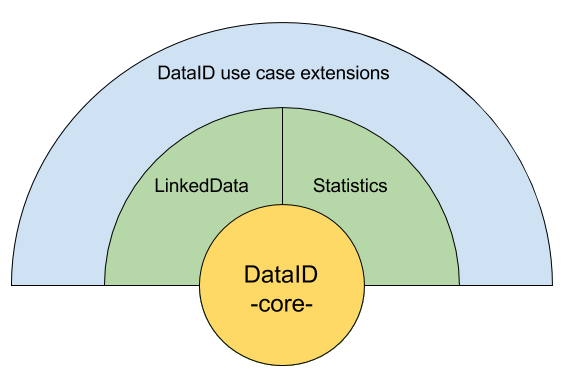
\includegraphics[width=9cm]{images/DataIDonionSliced.png}
  \caption{Example of combining multiple \dataid ontologies}
  \label{fig:onionslice}
\end{figure}

It may be necessary to add additional properties combined in a use case extension to satisfy all requirements.
This process will be the focus of the Data Management Plan use case presented in \Cref{chap:dmp}. In general, the usual recommendations for ontology engineering apply, when creating a use case extension for \dataid.

\begin{itemize}
\item Follow an established methodology when creating an ontology
\item Reuse well-established ontologies where possible (such as W3C recommended ontologies)
\item Create new classes based on more general concepts to harness additional functionality and increase interoperability (e.g. \prop{prov:Entity})
\item Make use of established tooling chains for modelling ontologies (such as Prot\'{e}g\'{e}\footnoteurl{http://protege.stanford.edu})
\item Provide sufficient documentation to ease understanding and reuse
\end{itemize}

In addition, I recommend the following:

\begin{itemize}
\item Keep the import portfolio as slim as possible - only import extensions or other ontologies which are really needed for the use case at hand to avoid semantic overlap.
\item Separate ontology from application profile - don't use the extension ontology for specifying use case specific restrictions, enter those into a second document. I recommend using the Shapes Constraint Language (SHACL) \cite{shacl} from the RDF Data Shapes W3C Working Group\footnoteurl{https://www.w3.org/2014/data-shapes/wiki/Main_Page} which is available as a working draft at the time of writing. This measure will aid the effort for Interoperability and Extensibility.
\item Specify mappings to other metadata formats at this stage to detect missing requirements. Reasons for this step might be already existing metadata files, or other metadata formats are needed for specific tasks such as a \ckan profile (\Cref{sec:ckan}) for publishing datasets on a data portal.
\end{itemize}

\paragraph{Generate DataID documents}
\label{sec:wfgenerate}

Creation of metadata documents is usually a task executed after the creation and before the publication of datasets. Nevertheless, there are multiple reasons not to wait until this stage to gather the necessary data:

\begin{itemize}
\item Describing source datasets is a task best done at a time before the extraction process, after source datasets have been studied.
\item The dataset creation process might take a long time, depending on the use case. Metadata for temporary result datasets can be useful for further extraction/transformation steps or to keep track of activities and agents involved (which is useful provenance metadata).
\item Quality measures and procedures can be accomplished with the toolchain dependent on a dataset and its metadata. Running such tasks in between extraction/transformation steps of data (and not only after the generation process is finished) is necessary to detect quality gaps early on.
\end{itemize}

When publishing a series of similar or versioned datasets, the automatic creation of \dataid documents becomes unavoidable. Integrating the creation of metadata as part of an automated workflow environment or ETL Framework (e.g. Unified Views \cite{KnapKMSTV14}) would be an obvious means of solving this issue.

As for the data generated, \dataid metadata needs validation to make sure of its correctness. While a syntactical validation of an RDF document is a necessary step, it is not sufficient. Tools for a semantic validation of an RDF graphs, against the ontology specified in the previous step, are available (e.g. RDFUnit \cite{rdfunit}).

\paragraph{Publish DataIDs alongside the datasets}
\label{sec:wfpublish}
Since dataset metadata is so indispensable for most consumers, the publication of \dataid metadata is released parallel to the publishing of datasets. \dataid was originally created under the assumption of metadata co-published alongside the datasets (\dataid files are in the same folder or at the root of a dataset file hierarchy). This is no longer a requirement since \core is expressive enough to find the associated dataset on the Web. However, storing metadata in proximity to its described dataset is good practice and eases the discoverability of both. 

Additionally, I propose the following best practice for publishing datasets on a given server:

Similarly to a \prop{robot.txt} file\footnoteurl{http://www.robotstxt.org}, I propose a file
to be put in the top-level directory of a server, named \prop{datacatalogs.txt}. Its content is a collection of relative paths, referencing files on the server, containing either an instance of \prop{dcat:Catalog}, pointing out datasets in turn, or instances of \prop{dcat:CatalogRecord} (e.g. \dataid{}s).
The format of these secondary files should be Turtle, which, in my opinion, is the RDF
serialisation featuring the best compromise between readability and file size. 

In example, next to the \url{http://dbpedia.org/robots.txt}
that explicitly excludes certain directories from being crawled,
the \url{http://dbpedia.org/datacalaog.txt} explicitly states where
metadata descriptions of \dbpedia datasets can be found. 
This best practice allows publishers to
reference descriptions of all hosted datasets in one place
and also enables users to discover and access these
datasets easily. It facilitates easy aggregation of an institution’s
or project’s datasets and massively cuts down on time
spent on navigating and searching for relevant datasets on
diverse websites.

\pagebreak
\paragraph{Exploitation of DataIDs}
\label{sec:wfexploit}
This stage summarises all activities of dataset consumers which are exploiting the benefits of the pertaining metadata as well. But exploitation is not limited to consumers alone. Data publishers, or pertaining organisations benefit from reliable and machine-readable metadata as well.

For example, the tables of the official download page for \dbpedia releases are all based on the \dataid documents accompanying the \dbpedia datasets\footnoteurl{http://wiki.dbpedia.org/downloads-2016-04}. Many other uses for \dataid documents are conceivable.

\section{Checklist for Publishing RDF Data} 
\label{sec:checklist}

The considerable experience members of the \dbpedia Association\footnoteurl{http://wiki.dbpedia.org/dbpedia-association} have gathered in regard to creation and dissemination of RDF data is presented in this section, summarising all important steps necessary for releasing such data. 
%Drawing from the publishing process for \dbpedia dataset releases, I  carved  out  a comprehensive checklist, offering guidance when producing and releasing RDF data. 
While this checklist is focused on Linked Data datasets, many items present could be generalised to fit broader use cases for any type of data. 
In addition, particular consideration has been given to tasks related to or dependent on dataset metadata (i.e. \dataid). I will highlight those items.

\paragraph{Documentation}
When publishing Linked Open Data, a comprehensive documentation of data sources, ontology, versioning and other important context needs to be presented in an easy and accessible manner. 
\begin{itemize}
\itemsep0em 
\item Decide early which form your documentation will take (online documentation, text files, etc.), depending on size or impact of a dataset. 
\item When preparing a new version of an existing dataset, list the coming changes to the dataset, as well as a release date.
\item Documentation is an iterative and never ending process. Therefore, improve documentation as early as possible to cover every aspect from the outset.
\item \textbf{\dataid}: Make sure to collect all references to documentation pages and append them to the pertaining dataset descriptions (e.g. with property \prop{foaf:page})
\item Facilitate means to gather feedback from dataset consumers (mailing list, issue tracker, etc.).%. Don't neglect feedback from consumers and provide support if needed.}
%\item{Discuss the extraction or generation process you employed to create RDF data. It might be useful for consumers to understand the steps involved. Procedural mistakes may come to light in the process.}
\item Record your plans on maintenance and versioning. A well maintained and regularly updated dataset will attract more consumers.%, regardless of the relevant information.}
\item Ask for support from your data consumers.
\end{itemize}

\vspace{-1.5em}
\paragraph{Sources}
Basing the generation of data on specific data sources is key for a coherent dataset release. 
A comprehensive documentation of the original sources should be one of the first steps in any data release.
\begin{itemize}
\itemsep0em 
\item \textbf{\dataid}: Metadata about the source data is highly desirable. Supplying consumers with additional information about the size of a probe, location, conditions, temporal information, dataset creator or publisher will further their understanding and acceptance of the data. It is useful to create a depiction of the source datasets with \core as well.
\item Name the exact version your release is based on. Do not divert from the selected version in the middle of your extraction.
\item Provide links to source files or host them yourself. Access to original data is vital for reproducibility. \textbf{\dataid}: use the concept of \prop{dataid:DatasetRelationship} together with the role \prop{dataid:SourceRole} to reflect this in the metadata.
\item Refer to external vocabularies \& ontologies utilized by your source data. Point to information about the schema of the source data.
\item Discuss quirks and unexpected issues you discovered about the source data.
\end{itemize}

\vspace{-1.5em}
\paragraph{Ontology \& Mappings}
\label{sec:less.onto}
Deciding on an ontology for the chosen domain is deciding on conceptual entities and relationships that will represent your data source. The appropriate level of abstraction is as vital as creating the mapping between both datasets. Note that all types of data extraction processes use mappings. Some mappings are obvious such as R2RML \cite{r2rml}, while others not so obvious (i.e. hidden in software code).

\begin{itemize}
\itemsep0em 
\item If no existing ontology can represent your data, engineer your own. Try using as many concepts of existing vocabularies as possible. \textbf{\dataid}: use property \prop{void:vocabulary} to refer your ontology.
\item Document any schema or mapping components. 
\item Before starting an extraction enrich and align your schema and mappings.
\item During an extraction use a static snapshot of used ontologies and mappings. These versions are the schematic foundation of your upcoming release and are not to be changed in the extraction and publishing process.

%\item Keep your consumers in the loop in this matter will enhance their experience with the data and offers the possibility to delegate the task creating and curating the ontology to an interested group of users (same for schema mappings). 
%\item When publishing a new dataset version, concentrate your curation efforts on weak spots in your ontology and mappings, which have emerged in previous versions.
\item Use a version control system to maintain your ontology and mappings. Especially large ontologies should be maintained by using a version control system like Git \footnote{\url{http://github.com}}.
\end{itemize}

\vspace{-1.5em}
\paragraph{Software}
Document exactly what kind of software, in what version is used for every step of the pre-processing, extraction and post-processing cycles.

\begin{itemize}
\itemsep0em 
\item When using custom software, use a version control system.
\item Provide sufficient information about the environment you are working with.
\item Provide additional information about deployment steps and configuration if necessary for the extraction process.
\item Create software snapshots to enable reproducibility of an extraction process.
\item \textbf{\dataid}: define your software in the context of \dataid as an agent who is responsible for the execution of certain transformation step. If a special software product is needed to process the data produced, state this with \prop{dataid:softwareRequirement}.
\end{itemize}

\vspace{-1.5em}
\paragraph{Extraction \& Dataset Generation}
While the generation process of an RDF dataset is a publisher-dependent process, there are some significant points to consider.

\begin{itemize}
\itemsep0em 
\item Prefer generating resulting datasets in different syntax formats. 
\item One triple per line is a preferred approach to enable easier procession of the RDF files with non-RDF tools (e.g. command-line directives).
\item Group RDF datasets by category or context. Break up large files, grouping triples by property. This way, subsets of properties, which are of no interest, can be left out of future tasks.
\item Use a consistent and precise naming strategy when creating files. File names should reflect exactly those triples stored inside (e.g. naming files by property and extraction step).
\item \textbf{\dataid}: Store provenance information alongside the files, preferably with your dataset metadata. Additional information about the origin or extraction steps leading to the triple will be useful in following tasks.
\item \textbf{\dataid}: Define the exact media type of your resulting files with \prop{dataid:MediaType}.
\end{itemize}

%\subsection{Post-Processing Steps}
%\emph{After the generation of RDF data some further steps are often necessary to straighten out minor issues[...?]. The main focus concerning this step is the validation and linking of the extracted data.}

\vspace{-1.5em}
\paragraph{Validation}
Validating extraction results to confirm their syntactic and semantic correctness is a necessary step, which will, in turn, confirm the correctness of ontology, mappings and the selected extraction process.
While validation should also be part of the extraction process itself (e.g. enforcing datatype conformance), most validation is done after the completion of an extraction step. An unsuccessful validation will trigger the cycle of 1) finding the fault, 2) fixing the problem and 3) rerunning the last extraction step(s).

\begin{itemize}
\itemsep0em 
\item Try to integrate validation directly in the extraction \& generation process to reduce post-validation steps.
\item Dataset size is an obvious indication of a release status. Finding obvious errors by comparing the size of a file with the size of previous versions.
\item A manual inspection of triples with sampling can identify errors early in the release process. 
\item Statistical metrics is a good means to provide an overview about quality. Information about both the source and the result data can provide a clear picture on how accurate an extraction performed. If a stark difference of equal types can not be explained by ontology or mappings, a bug in the extraction process is the probable answer. 
\item Create your own validation tools and use external, general purpose RDF validation tools.
\item Use a staging SPARQL endpoint and/or linked data interface for browsing the data.
\item Tools, such as RDFUnit \cite{rdfunit}, perform ontology conformance tests and should be used for a thorough validation of your data.
\item \textbf{\dataid}: Any validation result of your data is valid metadata, which can be stored in your \dataid{}s. (e.g. with Data Quality Vocabulary cf. \Cref{sec:extensions}).
\end{itemize}

\vspace{-1.5em}
\paragraph{Enrichment}
Dataset enrichment with information from other data sources is a useful step to increase the precision and/or coverage of a knowledge base.
However, Enrichment is a step that is closely coupled to a dataset and is therefore no specific advice in this regard.
%While structured source data rarely demand for enrichment, un- or semistructured sources might. There is no precise guide to be given concerning this point. Possible enrichment has to be identified with the help of ontology and mappings.

\begin{itemize}
\itemsep0em 
\item RDFS or OWL inferencing using the main or external schemata is definitely a means to add missing knowledge
\item Dataset-dependant heuristics can be employed
\item Different types of enrichment can be performed before and after the \emph{linking} step but in most case must be done prior to validation.
\end{itemize}


\vspace{-1.5em}
\paragraph{Linking}
As a basic principle of Linked Open Data \cite{5starData},
, linking is one of the most important steps in the process of creating RDF datasets.
This can be achieved by multiple approaches:

\begin{itemize}
\itemsep0em 
\item{Performing a manual linking over time. (tends to be a very limited solution)}
\item{Copying existing link sets from other datasets to previous versions of the extracted dataset (which will be outdated).}
\item{Detecting identifiers pertaining to entities of the source or result datasets in different datasets. Generating owl:sameAs triples would complete this method.}
\item By using the transitive trait of owl:sameAs.% [Finding a link pointing from set1:e1 -> set2:f1 and set2:f1 -> set2:k3 is equivalent to  set1:e1 -> set2:k3.]}
\item{Provide interlinks between same resources in a dataset (e.g. in different language editions)}
\item \textbf{\dataid}: Provide instances of concept \prop{dataid-ld:Linkset} to point out the involved datasets (between which links were found) and additional information such as link predicate and number of links found.
\end{itemize}

\vspace{-1.5em}
\paragraph{Publishing}
Publishing a dataset is a complex task, which can be done in many ways. 
Providing raw RDF data alone is not enough to disseminate Linked Open Data.

\begin{itemize}
\itemsep0em 
\item Update user documentation (e.g. online data catalogues - i.e. datahub.io).
\item Announce the release at different venues. 
\item Upload your dump files to an accessible location with consistent serialization formats.
\item If possible, make the data available through a SPARQL Endpoint and/or a Linked Data interface.
\item \textbf{\dataid}:  Publish/update metadata documents, to provide a comprehensive dataset description. Providing a metadata such as \dataid will increase the visibility of your data and automatically create link sets to other datasets.
\item \textbf{\dataid}: Store the created \dataid documents a) alongside your created datasets, as well as in data portals specialised for \dcat metadata or convert into other metadata formats if needed.
\end{itemize}


\chapter{Application: Data Management Plans (DMP)}
\label{chap:dmp}
Over the last years, Data Management Plans (\dmp) have become a requirement for project proposals within most major research funding institutions. It states what types of data and metadata are employed, which limitations apply, where responsibilities lie and how the data is stored, both during research project and after the project is completed. 

The use case described here will introduce an extension to the \core ontology to extensively describe a Data Management Plan for digital data in a universal way, laying the foundation for tools helping researchers and funders with the drafting and implementing of \dmp{}s.
Based on multiple requirements, raised from different \dmp guidelines, I will showcase the creation of a \dataid extension. I incorporated the \redata ontology to describe repositories and institutions, exemplifying the use of external ontologies. This approach will demonstrate the application of the best practices introduced in \Cref{sec:composingmetadata} for the stages 'Specify' and 'Model' of the lifecycle for dataset metadata. Furthermore, this use case exemplifies the ability of the \ecosystem to solve complex demands on dataset metadata based on its trait of Extensibility.
%A concise summary of how we solved all of our requirements finalises this section.

\section{Specifying requirements of a DMP} 
\label{sec:dmprequ}
The following requirements were distilled from an extensive list of \dmp guidelines of different research funding bodies, covering most of the non-functional demands raised pertaining to digital datasets. 

\begin{enumerate}
\item Describe how data will be shared (incl. repositories and access procedures). %and embargo periods (if any). 
\item Describe the procedures put in place for the long-term preservation of the data.
\item Describe the types of data and metadata, as well as identifiers used.
\item Provisioning of copyright and license information, including other possible limitations to the reusability of the data.
\item Outline the rights and obligations of all parties as to their roles and responsibilities in the management and retention of research data.
\item Provision for changes in the hierarchy of involved agents and responsibilities (e.g. a Primary Investigator (PI) leaving the project).
\item Include provenance information on how datasets were used, collected or generated in the course of the project. Reference standards and methods applied.
\item Include statements on the usefulness of data for the wider public needs or possible exploitations for the likely purposes of certain parties.
\item Provide assistance for dissemination purposes of (open) data, making it easy to discover it on the web.
\item Is the metadata interoperable allowing data exchange between different metadata formats, researchers and organisations?
\item Project costs associated with implementing the \dmp during and after the project. Justify the prognosticated costs.
\item Support the data management life cycle for all data produced.
\end{enumerate}

Guidelines and checklists on Data Management Plans of different research (related) organisations were surveyed to generate this list of requirements. The most influential guidelines to this process are listed below. References like \textbf{(R1)} refer to the requirements listed above and connects guidelines or checklists to a requirement respectively. A complete list of involved organisations is available on the Web\footnoteurl{http://wiki.dbpedia.org/use-cases/data-management-plan-extension-dataid\#Organisation}.

\begin{enumerate}
\item \textbf{Horizon 2020 (H2020)}: Horizon 2020 is a framework programme of the European Commission funding research, technological development, and innovation\footnoteurl{https://ec.europa.eu/programmes/horizon2020/}. (\dmp guidelines\footnoteurl{https://ec.europa.eu/research/participants/data/ref/h2020/grants_manual/hi/oa_pilot/h2020-hi-oa-data-mgt_en.pdf})

\item \textbf{National Science Foundation (NSF)}: The National Science Foundation\footnoteurl{http://www.nsf.gov/} is a United States government agency that supports fundamental research and education in all the non-medical fields of science and engineering. (\dmp guidelines\footnoteurl{http://nsf.gov/eng/general/ENG_DMP_Policy.pdf})

\item \textbf{Economic and Social Research Council (ESRC)}: The Economic and Social Research Council\footnoteurl{http://www.esrc.ac.uk/} is one of the seven Research Councils in the United Kingdom and provides funding and support for research and training work in social and economic issues. (\dmp guidelines\footnoteurl{http://www.esrc.ac.uk/funding/guidance-for-grant-holders/research-data-policy/})

\item \textbf{Deutsche Forschungsgemeinschaft (DFG)}: The DFG is the largest independent research funding organisation in Germany. It promotes the advancement of science and the humanities by funding research projects, research centres and networks. (\dmp guidelines\footnoteurl{http://www.dfg.de/download/pdf/foerderung/antragstellung/forschungsdaten/richtlinien_forschungsdaten.pdf})

\item \textbf{Inter-university Consortium for Political and Social Research (ICPSR)}: ICPSR\footnoteurl{https://www.icpsr.umich.edu/} advances and expands social and behavioural research, acting as a global leader in data stewardship and providing rich data resources and responsive educational opportunities. (\dmp guidelines\footnoteurl{http://www.icpsr.umich.edu/files/datamanagement/DataManagementPlans-All.pdf})

\item \textbf{UK Data Archive}: The UK Data Archive\footnoteurl{http://www.data-archive.ac.uk/} is the curator of the largest collection of digital data in the social sciences and humanities in the United Kingdom. (\dmp checklist\footnoteurl{http://www.data-archive.ac.uk/create-manage/planning-for-sharing/data-management-checklist})
\end{enumerate}

\begin{table}[!htbp]
    \centering
    \begin{tabular}{|l|c|c|c|c|c|c|c|c|c|c|c|c|}
        \hline
         & R1 & R2 & R3 & R4 & R5 & R6 & R7 & R8 & R9 & R10 & R11 & R12 \\
        \hline
        H2020 & \checkmark & \checkmark & \checkmark & \checkmark &  & \checkmark &  &  & \checkmark & \checkmark & \checkmark & \checkmark\\
        NSF & \checkmark & \checkmark & \checkmark & \checkmark & \checkmark & \checkmark &  & \checkmark & \checkmark &  & \checkmark &  \\
        ESRC &  & \checkmark &  & \checkmark & \checkmark &  & \checkmark &  &  &  &  &  \\
        DFG & \checkmark & \checkmark &  & \checkmark &  &  &  &  &  &  & \checkmark &  \\
        ICPSR & \checkmark & \checkmark & \checkmark & \checkmark & \checkmark &  &  &  & \checkmark & \checkmark & \checkmark & \checkmark \\
        UKDA &  & \checkmark & \checkmark & \checkmark & \checkmark &  & \checkmark &  &  &  & \checkmark &  \\
        \hline
    \end{tabular}
    \caption{\dmp requirements of research (related) institutions (selection)}
    \label{tab:institutions}
\end{table}

To implement these demands in an ontology, the following implications are already evident:
\begin{enumerate}
\item making further use of \prov is necessary to deal with the extensive demands for provenance,
\item a clear specification of involved agents and their responsibilities is needed, 
\item an extensive description of repositories retaining the described data is inescapable.
\end{enumerate}

My goal is to provide aid for researchers in drafting a \dmp and implementing it with all requirements in mind: during the proposal phase, while the project is ongoing and the long-term implementation of the \dmp.

\section{Modelling the DataID approach} 
\label{sec:dmpmodel}

The final \dmp use case extension, created to resolve the requirements listed in the last section, will extend \core together with the existing extension \textit{Activities \& Plans} and the repository ontology of \textit{re3data.org} (cf. \Cref{sec:re3data}). All three ontologies will be outlined in this section in a concise manner. For an exhaustive description, please refer to the online documentation referenced below. 

\paragraph{Activities \& Plans} To utilise the full breath of provenance offered by \prov and adding further semantics to satisfy all provenance related requirements is the purpose of this extension, providing the means to record all steps which are necessary to recreate a certain dataset, given the same data sources.
Besides \prov and \core, it imports the following ontologies:

\begin{description}
\item[\dlo] The Data Lifecycle Ontology (cf. \Cref{sec:dlo}) is used to define stages of the data management lifecycle. By combining both ontologies of the data engineering side of the ALIGNED project (i.e. \dlo and \core) \cite{SolankiBFKDB16}, I established the means to portray datasets (or any data artefact) in the context of the data management life-cycle. 
\item[\org] The Organization Ontology (cf. \Cref{sec:org}) extends \core with important context information about the organisational background of involved Agents, which is an important detail when describing the interplay of \important{Agents} and \important{Activities}.
\end{description}
\begin{figure}
\vspace*{-1.5cm}
\centering
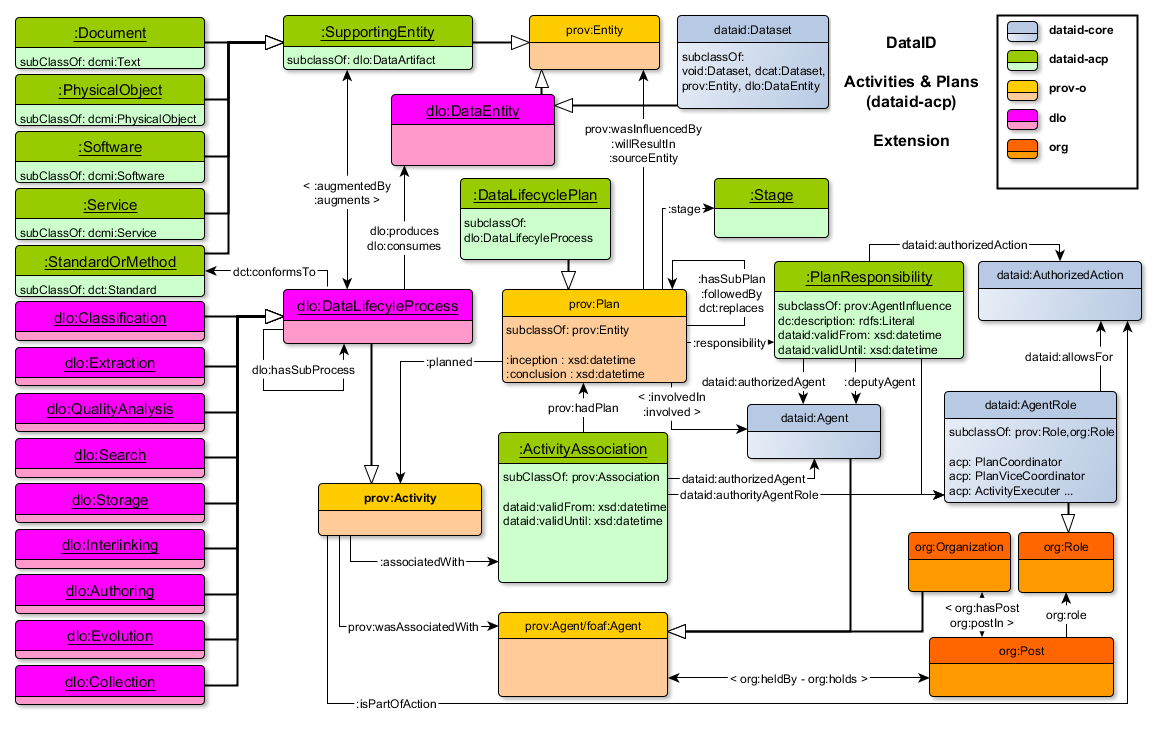
\includegraphics[angle=90, width=\textwidth]{images/ActivityPlansExt.png}
  \caption{Activities \& Plans extension}
  \label{fig:acp}
%\floatfoot{This ontology is accessible here: \url{https://github.com/dbpedia/DataId-Ontology/blob/DataManagementPlanExtension/dmp/dataManagementPlanExt.ttl}}
\end{figure}

To integrate DLO in the existing landscape of \dataid and \prov concepts (\Cref{fig:acp} - specification:\footnoteurl{https://github.com/dbpedia/DataId-Ontology/blob/07a6a1795637973a921a37f086d0e4f57968b1d5/acp/activitiesPlansExt.ttl}), I extended the list of sub-class axioms for \prop{dataid:Dataset}, to inherit \prop{dlo:DataEntity}\footnote{Note: this is no ontology hijacking, since one reason for creating the \ecosystem was to provide a controlled environment for redefining concepts or properties in the extension (cf. \Cref{sec:landscaping}).}.
DLO is used to classify different types of activities (\prop{dlo:LifeCycleProcess}) and to adopt its basic semantics for an exchange of data artefacts between activities. Similar to \prop{dataid:associatedAgent} and \prop{dataid:Authorization} (cf. \Cref{sec:coreauthorization}), the property \prop{prov:wasAssociatedWith} is further qualified by the class \prop{dataid-acp:ActivityAssociation}, reusing relevant properties for this kind of mediator (such as \prop{dataid:authorizedAgent}). This class can not only qualify a generic association with an \important{Agent}, \important{AgentRole} and a time interval but provides the means of referencing a \prop{prov:Plan}, which was responsible for the scheduling of an \important{Activity} in the first place.

\important{Plans} offer the necessary properties to (pre-) define a sequence of \important{Activities}, governed by \important{Agents} (with responsibilities), which are generating \important{Entities}. An instance of \prop{prov:Plan} is constituted of multiple sub-plans, which have a defined order. This order specifies when an \important{Activity} is executed. While \prop{dataid-acp:ActivityAssociation} (and its associated \important{AgentRole}) specifies responsibilities for a specific \important{Activity}, \prop{dataid-acp:PlanResponsibility} defines responsibilities of \important{Agents} regarding the \important{Plan} itself (such as defining the order of \important{Activities} etc.).

\paragraph{The re3data.org ontology} To cover the requirements for preservation (e.g. \textbf{(R1)}), a comprehensive description of repositories is necessary. The \redata schema \cite{r3dSchema} (cf. \Cref{sec:re3data}) does provide a thorough description of repositories and the unique opportunity to incorporate an existing, up-to-date collection of research repositories in future \dataid{}-based applications. To accomplish the integration into the \dmp ontology extension, I transformed the current XML-based schema into an OWL-ontology, using established vocabularies like \prov and \org. The schema, as well as the data provided by \redata, will be available as Linked Data (e.g. via \redata ReSTful-API), thus making it discoverable and more easily accessible for services and applications, reaching a larger circle of users. This effort was support generously by the re3data.org project.

\begin{figure}
\vspace*{-1.0cm}
\centering
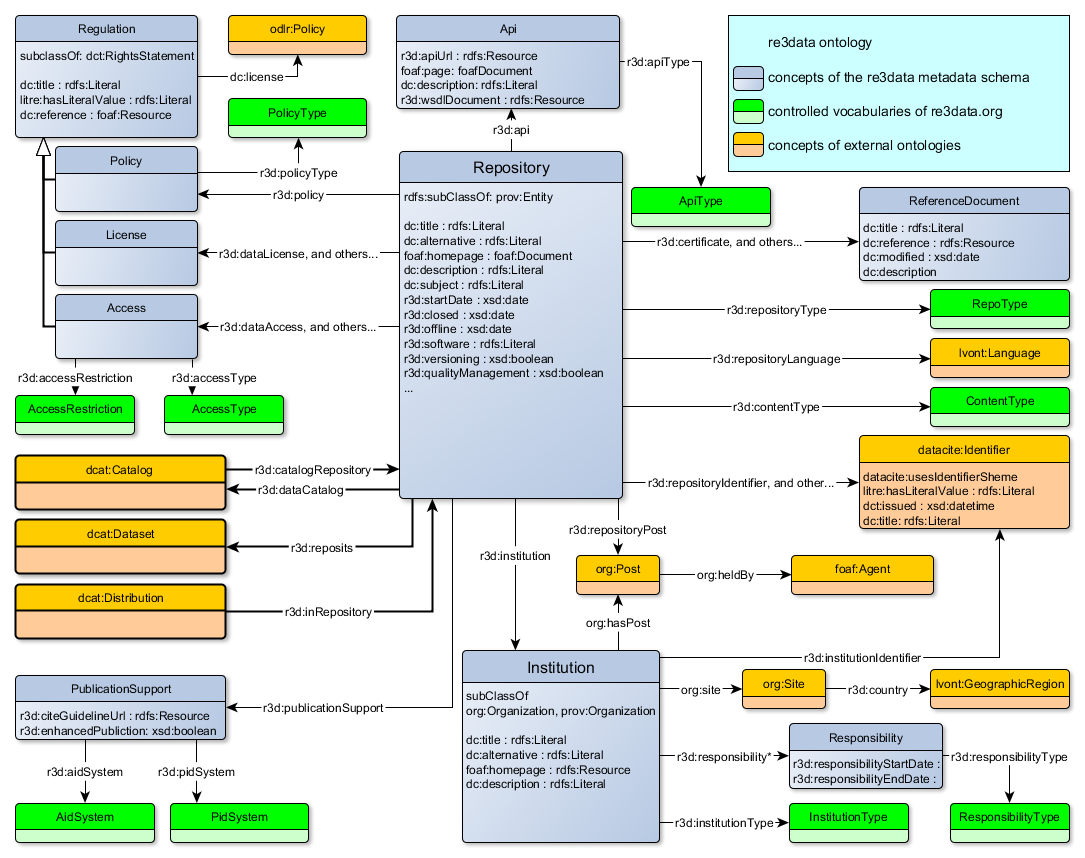
\includegraphics[angle=90, width=\textwidth]{images/r3dOntologyReduced.png}
  \caption{re3data.org ontology}
  \label{fig:re3data}
\floatfoot{Note: This is a reduced depiction of the ontology omitting some properties
and all instances of controlled vocabularies (green boxes). A complete depiction is available here:\\
\url{https://github.com/re3data/ontology/blob/master/visuals/r3dOntology.png}\\
The current version can be accessed here:\\ 
\url{https://github.com/re3data/ontology/blob/master/r3dOntology.ttl}}
\end{figure}

Alongside the repository concept, a rudimentary description of institutions which are hosting or funding a repository is needed to ensure long-term sustainability and availability of a repository. The derived \redata ontology (\Cref{fig:re3data}) supplements \prop{r3d:Repository} and \prop{r3d:Institution} with fitting \prov sub-classes 
(\prop{prov:Entity}, \prop{prov:Organization}),
making them subject to provenance descriptions. The \org ontology is used to extend the institution class further, providing organisational descriptions.

In the ontology version of the \redata schema, I tried to combine multiple similarly structured XML elements into a single concept, where possible.
For example, access regulations to the repository and the research data must be clarified, as well as the terms of use. The \redata ontology unifies all license and policy objects under the class \prop{r3d:Regulation}, using the property \prop{dct:license} to point out \prop{odrl:Policy} descriptions of licenses, as used in the \core ontology.
The ranges of multiple properties (i.e. \prop{r3d:certificate}, \prop{r3d:metadataStandard} and \prop{r3d:syndication}) were bundled to form \prop{r3d:ReferenceDocument} (a sub-class of \prop{foaf:Document}).

As with \core, I tried to replace commonly used concepts with existing classes of well-established vocabularies. Property \prop{r3d:repositoryLanguage} is pointing out instances of class \prop{lvont:Language} (of the Lexvo ontology  - cf. \Cref{sec:lexvo}) and properties calling for identifier like structures are referencing instances of \prop{datacite:Identifier} (a natural fit, due to the fact that re3data.org is now under the care of DataCite).

By linking to \prop{dcat:Catalog} via \prop{r3d:dataCatalog} and \prop{dcat:Dataset} with \prop{r3d:reposits}, we introduced the necessary means to relate descriptions of data stored in a repository. By providing this interface with the \dcat vocabulary, \dataid can be used for the description of data in the \redata context.

%The DataID core ontology, the Activities \& Plans extension (cf. \Cref{dataid}) and the re3data ontology are the foundational components of the \dmp extension (depiction: \Cref{fig:dmp}). 
%(references like \textbf{(R1)} correspond to those requirements).
\paragraph{The DMP use case Extension}

On top of these foundational components, we added an additional semantic layer, solving the requirements listed in \Cref{sec:dmprequ}, creating the \dmp use case extension (specification: \footnoteurl{https://github.com/dbpedia/DataId-Ontology/blob/07a6a1795637973a921a37f086d0e4f57968b1d5/dmp/dataManagementPlanExt.ttl}).
Extensive use of the \prov ontology and the concepts and properties introduced by the \textit{Activities \& Plans} extension is key to \dmp, providing the means for describing sources and origin activities of datasets \textbf{(R7)}. 

\begin{figure}[!htbp]
\centering
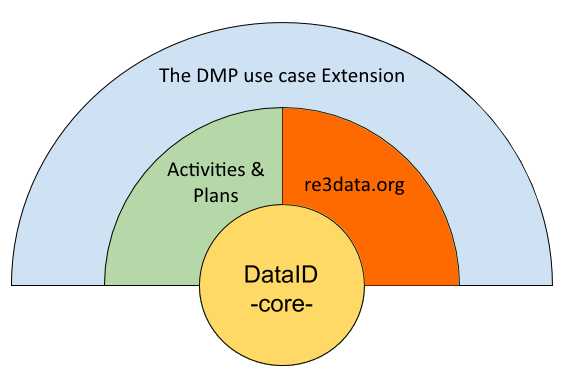
\includegraphics[width=10cm]{images/DataIDonionDmp.png}
  \caption{\dmp use case}
  \label{fig:dmp}
\floatfoot{Note: The \redata ontology is of cause not part of the common layer of the \ecosystem and does not import \core. The placement of ontologies was chosen for convenience.}
\end{figure}

In the same vein, using the \prop{dataid:Authorization} concept, augmented with a \dmp specific set of \prop{dataid:AgentRole} and \prop{dataid:AuthorizedAction}, adds necessary provenance and satisfies requirement \textbf{(R5)} and \textbf{(R6)}.

\begin{figure}
\vspace*{-0.8cm}
\centering
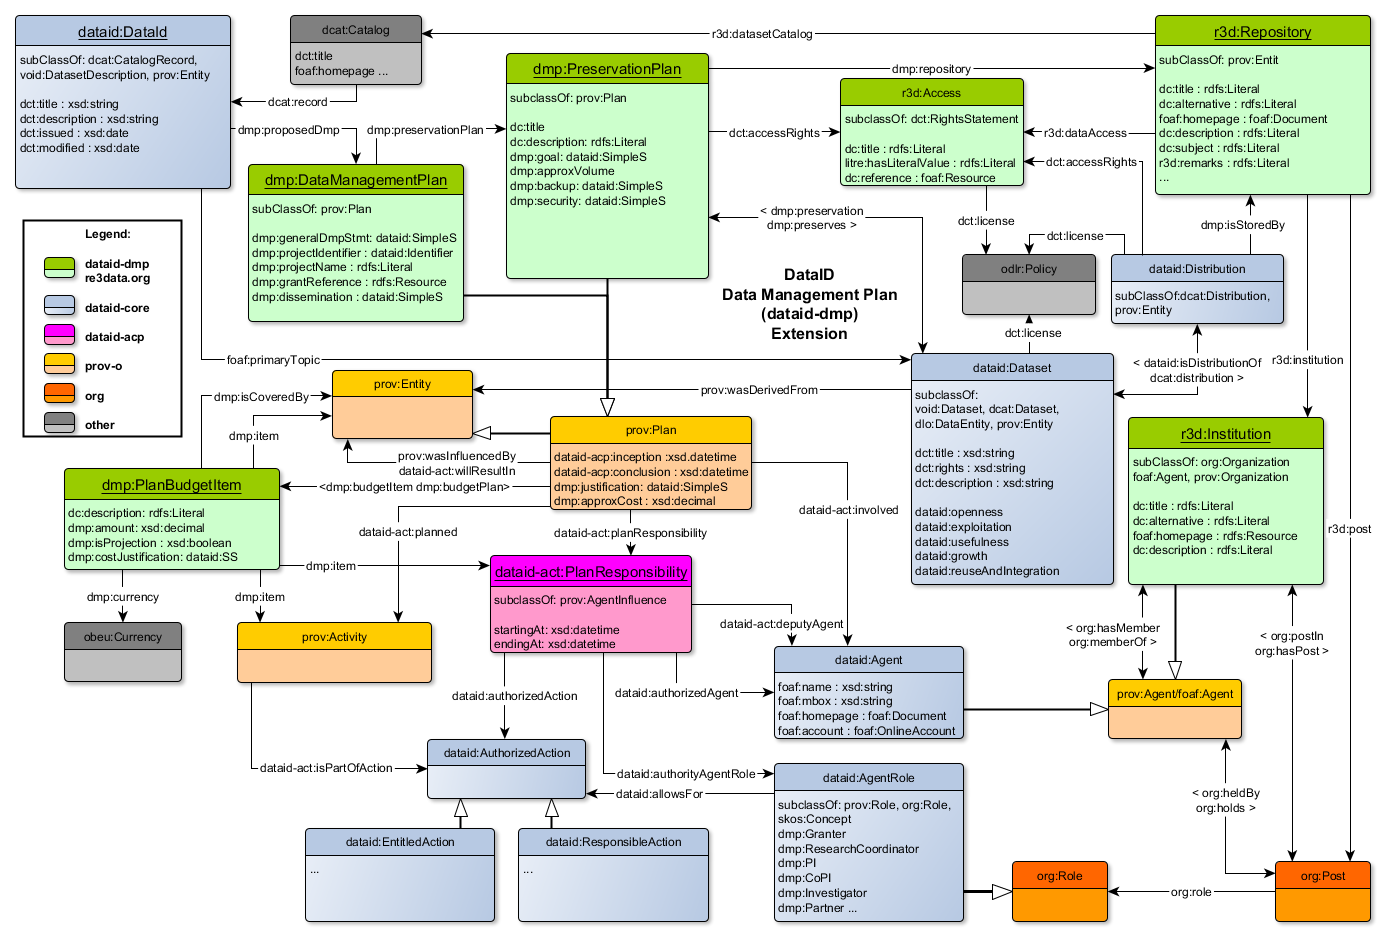
\includegraphics[angle=90, width=\textwidth]{images/DmpOntologyExt.png}
  \caption{\dmp use case extension}
  \label{fig:dmp}
%\floatfoot{This ontology is accessible here: \url{https://github.com/dbpedia/DataId-Ontology/blob/DataManagementPlanExtension/dmp/dataManagementPlanExt.ttl}}
\end{figure}

A description of repositories involved in a \dmp is provided by the concept \prop{r3d:Repository}, including exact documentation of APIs and access procedures \textbf{(R1)}. More detailed information on the type of data or additional software necessary to access the data was introduced with \prop{dataid:Distribution}.

As in DataID core, information about licenses and other limitations are provided via \prop{dct:license} and \prop{dct:rights} \textbf{(R4)}, or the complementary properties of the re3data ontology concerning access and other policies.
Helpful information on usefulness, reusability and other subjects for possible users of the portrayed datasets are added to the \prop{dataid:Dataset} concept: \prop{dataid:usefulness}, \prop{dataid:reuseAndIntegration}, \prop{dataid:exploitation} etc. \textbf{(R8)}.

Requirement \textbf{(R3)} is intrinsic to DataID and needs no further representation, while \textbf{(R10)} is exemplified by the next chapter (\Cref{chap:map}). 

The heart of the \dmp extension (\Cref{fig:dmp}) are two subclasses of \prop{prov:Plan}:
The \prop{dmp:DataManagementPlan} provides the most general level of textual statements about the \dmp itself or the planned dissemination process \textbf{(R9)}, as well as the necessary references to pertaining projects. While \prop{dmp:PreservationPlan} entities can describe different approaches for the preservation of different datasets \textbf{(R2)} or provide temporal scaling (e.g. regarding embargo periods). Besides textual statements about general goals and provisions for security and backup, using the \prop{dataid-acp:planned} property to point out specific tasks, put in place to preserve data long term, is one of the more notable provenance information.
%provided with \dmp.

The concept \prop{dmp:BudgetItem} is an optional tool to list costs of activities, responsibilities (consequently costs of agents) and any entity involved in a plan like \prop{dmp:PreservationPlan}. Together with \prop{dmp:approxCost} and\hfill \break \prop{dmp:justification} it satisfies requirement \textbf{(R11)}.

Several functional requirements raised by the guidelines of research funding bodies (which are not included in the requirements of this section) will be covered by the \dataid service (cf. \Cref{chap:future}). It will provide a versioning system for \dataid{}s (based on properties like \prop{dataid:nextVersion}), enabling features like tracking changes to a \dataid over time.
%the current implementation status of a \dmp. 
Thereby, the full Data Management Lifecycle of datasets is supported \textbf{(R12)}. Not only by the formal description with dataset metadata but by the tooling being created around it. 

\section{Summary} 
\label{sec:dmpsummary}
I created 3 classes and 17 properties for this use case extension, which, together with the concepts and properties introduced by the \redata ontology and the \textit{Activities \& Plans} extension, can describe Data Management Plans as demanded by the requirements of \Cref{sec:dmprequ}. 
%(e.g. the English \dbpedia dataset\footnoteurl{http://downloads.dbpedia.org/2015-10/core-i18n/en/2015-10_dataid_en.ttl}).

This approach of extending and specialising the use of \core, while reusing (partial) solutions to more specific problems, demonstrates the capability of the \ecosystem to adapt to any use case for dataset metadata, without impacting the kernel nature of \core. Thereby, proving its Extensibility.

This section demonstrated the first two stages of the engineering lifecycle for \dataid metadata parallel to its counterparts in the Data Management Lifecycle (cf. \Cref{sec:composingmetadata}). The stages of \textit{Generate, Publish and Exploit} are outside of the scope of this document.


\chapter{The Interoperability of DataID}
\label{chap:map}

This section is focused on the Interoperability of \core with other dataset metadata vocabularies. As discussed in \Cref{sec:extensvsinter}, Interoperability is more easy to establish, when interoperating with an upper (general) ontology. 
In the case of \dataid, Interoperability is achieved on a semantic level (the fourth level of conceptual interoperability - cf. \Cref{sec:interoperability}) without consideration for contextual restrictions on properties. Vocabularies imported into \core are conceivably easy to interoperate with, since an agreement on the metadata format exists (i.e. Dublin Core, \dcat, \prov, \void). Other vocabularies need a metadata mapping to achieve full Interoperability.

\section{DCAT Application Profile} 
\label{sec:mapdcatap}

I will demonstrate how easy a metadata mapping can be achieved between \core and another \dcat{}-based vocabulary. \dcatap is an application profile (cf. \Cref{sec:dcatap}) of \dcat which also imports the \adms (cf. \Cref{sec:adms}), Dublin Core and other vocabularies \cite{dcatap11}. Properties of the \dcat or Dublin Core vocabularies only need minimal attention to achieve a mapping. In fact, only those properties which are restricted in range (such as \prop{dct:license}, \prop{dcat:mediaType} or \prop{dct:language}) are of concern. Others need no mapping at all. Since \dcatap uses the same basic concept structure and the same levels of abstraction, no special consideration of redistributing properties over different concepts with different meanings has to be undertaken. When converting \dataid metadata to \dcatap, information about \important{Authorizations} and all pertaining concepts are lost. Some associated agent relations might be converted to standard properties such as \prop{dct:publisher} or \prop{dct:maintainer}.

When converting into a \dataid, properties of the \adms vocabulary, reused by \dcatap, will need either a mapping or are otherwise dealt with. 
%Properties of \spdx can easily be reused, since this ontology is only used in connection with checksums in both vocabularies.
The easiest way to resolve most of the issues in this particular instance, would be to extend \core with the \adms vocabulary if the surrounding circumstances would allow for this change.

This is the list of all properties of the \dcatap vocabulary, which would need a mapping (or other actions) to interoperate safely with \core:

\begin{table}[!htbp]
    \centering
    \begin{tabular}{|l|l|}
        \hline
        property & reason or possible solution \\
        \hline
        \prop{adms:status} & missing equivalent\\
        \prop{adms:identifier} & property mapping: \prop{dataid:identifier}\\
        \prop{adms:sample} & property mapping: \prop{void:exampleResource}\\
        \prop{adms:versionNotes} & missing equivalent\\
        \prop{dct:license} & range restriction: \prop{odrl:Policy}\\
        \prop{dct:rights} & range restriction: \prop{dataid:SimpleStatement}\\
        \prop{dct:accessRights} & range restriction: \prop{dataid:SimpleStatement}\\
        \prop{dct:conformsTo} & range restriction: \prop{dataid:SimpleStatement}\\
        \prop{dct:provenance} & range restriction: \prop{dataid:SimpleStatement}\\
        \prop{dct:language} & range restriction: \prop{lvont:Language}\\
        \prop{dct:format} & property mapping: \prop{dcat:mediaType}\\
        \prop{dct:identifier} & property mapping: \prop{dataid:literal}\\
        \prop{skos:notation} & property mapping: \prop{dataid:literal}\\
        \hline
    \end{tabular}
    \caption{Properties of the \dcatap vocabulary in need of a mapping to \core}
    \label{tab:dcatapmapping}
\end{table}

Possible resolutions:
\begin{description}
\item[missing equivalent:] \core has no suitable property to reflect this information. To resolve this mapping, either an extension to \core is constructed, an unused property (e.g. from \dcat) is re-purposed (which I strongly discourage) or it is neglected all together.
\item[property mapping:] An existing property is available in \core to convey this kind of information. In where the ranges of both properties do not match, a transformation of the object instance/value has to be performed (see next item).
\item[range restriction:] \core imposes a range restriction on this property. As a result, the values used with \dcatap often need to be transformed into an instance of the concept it is restricted to (e.g. for \prop{dct:language}: literal "en" transformed to <http://lexvo.org/id/iso639-3/eng>).
\end{description}

I will not produce an actual mapping here. It is obvious that the extend of this effort can not be immense. One advantage of basing \dataid on \dcat is the evident ease in with many metadata formats can be interoperated with.

\pagebreak
\section{Component MetaData Infrastructure (CMDI)} 
\label{sec:mapcmdi}
This section exemplifies how diverse metadata formats like \cmdi can easily be transformed into a \dataid, by providing a metadata mapping between them. 
%or supported authorisation levels, where it is expected that the DataID vocabulary will help building a more complete metadata stock. 

The variety of supported resource types by this component-based framework (cf. \Cref{sec:cmdi}), may lead to a substantial effort in aligning existing instances to their \dataid counterparts. 
Earlier work on the conversion of \cmd profiles into RDF/RDFS\cite{DW2014} reflects the complete bandwidth of \cmdi-based metadata, but also some idiosyncrasies that may constrain its usage in other contexts. It is expected that a transformation of relevant data to a uniform, \dataid{}-based vocabulary will enhance visibility and exploitation of \cmdi resources in new communities.
Despite the fact that currently more than 80 \cmd profiles are actually in use, the amount of metadata instances created on their basis, is far from being equally distributed. 
%The four most popular \cmd profiles are used as schemata for around 56\% of all publicly available metadata files. 
I created explicit mappings for \cmd profiles, accountable for 56\% of all publicly available metadata files, matching the appropriate \dataid classes and applied them on all respective instance files via XSPARQL\footnoteurl{https://www.w3.org/Submission/xsparql-language-specification/}. An overview of created mappings can be found on Github\footnoteurl{https://github.com/dbpedia/Cmdi-DataID-mappings}. 

\begin{table}[!htbp]
    \centering
    \begin{tabular}{l|p{3cm}|p{3cm}|p{3cm}}
        \hline
        \cmd profile & \cmd instances (in \% of all) & Supported properties of dataid:Dataset & Supported dataid:AgentRoles \\
        \hline
        OLAC-DcmiTerms & 156.210 (17,4\%) & 13 & 3 \\
        Song & 155.403 (17,3\%)& 9 & 1 \\
        imdi-session & 100.423 (11,2\%) & 9 & 2 \\
        teiHeader & 87.533 (9,7\%)& 10 & 2 \\
    \end{tabular}
    \caption{Most popular \cmd profiles and their completeness regarding DataID classes}
    \label{tab:cmdi_profiles}
\end{table}

The creation and further adaptation of these mappings showed that the support of data considered essential in \dataid differs between all profiles. The summary table \ref{tab:cmdi_profiles} demonstrates this effect for primary properties of \prop{dataid:Dataset} and the support of different \important{AgentRoles} specified in \prop{dataid:Agent}. Apparently there is a varying degree of conformance of both approaches, indicating possible shortcomings in specific \cmd profiles. An example for such a potential deficit is the fine-grained modelling of involved persons or organisations via \dataid{}'s Agent concept that is only partially supported in most profiles.
Some \cmd profiles can not be covered solely with \core. In these cases, an specific extension (or the reuse of existing \dataid extensions) is necessary to convey the complete metadata document with \dataid.


\chapter{Evaluation}
\label{chap:evaluation}

\section{Publishing DBpedia datasets with DataID metadata} 
\label{sec:evaldbpedia}
In this first approach to evaluate \dataid, I want to have a closer look on the already presented example of \dbpedia datasets (cf. \Cref{sec:coreclasses}) in affiliation with \dataid metadata. Therefore, this section will not only evaluate metadata specific aspects of this example, but tries to measure the overall effect of better metadata on datasets.
\todo{maybe rephrase} 
I will do so by evaluating against the best practices presented by the W3C 'Data on the Web' working group and the FAIR Principles (cf. \Cref{sec:fair}). In both cases I will gauge each practice by its state of fulfilment for the \dbpedia use case. I will assign one of the following ratings to every practice: \textbf{(2)} The requirement is supported in full. \textbf{(1)} The requirement is partially met. \textbf{(0)} \dbpedia does not support this requirement. A short statement will explain the decision. While this is an evaluation of the \dbpedia datasets against these practices, many of them are dependent on the \dataid documents, published alongside the datasets, for completion. To point out these instances, a second look at these particular practices is taken in \Cref{sec:evaldataid}.

\subsection{Data on the Web Best Practices} 
\label{sec:evaldwbp}
This collection presented by the 'Data on the Web' (DWBP) W3C working group\footnoteurl{https://www.w3.org/2013/dwbp/wiki/Main_Page} and their best practices document \cite{dwbpW3C2016} (released as recommendation candidate by the time of writing) is the most comprehensive selection of best practices on data publishing available (cf. \Cref{sec:bestprctice}). Fortunately, the 'Data on the Web' working group decided early on to include \dbpedia as a candidate in their implementation report. The following evaluation of \dbpedia with \dataid was done in collaboration with the W3C working group. A complete table of this evaluation is available on the Web\footnoteurl{http://dataid.dbpedia.org/ns/dwbp.html}. 

\begin{description}
 \item[1. Provide metadata] \textit{Provide metadata for both human users and computer applications.} - \dataid is dataset metadata.
 \hfill\textbf{\color{ForestGreen}(2)}
 \item[2. Provide descriptive metadata] \textit{Provide metadata that describes the overall features of datasets and distributions.} - This is the basic idea of \dataid.
\hfill\textbf{\color{ForestGreen}(2)}
 \item[3. Provide structural metadata] \textit{Provide metadata that describes the schema and internal structure of a distribution.} - \dataid can portray this with \prop{void:vocabulary} and the information available through \prop{dataid:MediaType}.
\hfill\textbf{\color{ForestGreen}(2)}
 \item[4. Provide data license information] \textit{Provide a link to or copy of the license agreement that controls use of the data.} - This is achieved with instances of \prop{odrl:Policy}.
\hfill\textbf{\color{ForestGreen}(2)}
 \item[5. Provide data provenance information] \textit{Provide complete information about the origins of the data and any changes you have made.} - This is a central concept of \core.
\hfill\textbf{\color{ForestGreen}(2)}
 \item[6. Provide data quality information] \textit{Provide information about data quality and fitness for particular purposes.} - Data quality can not be represented with \core. Yet, a data quality extension is already planned (cf. \Cref{chap:future}).
\hfill\textbf{\color{Mahogany}(0)}
 \item[7. Provide a version indicator] \textit{Assign and indicate a version number or date for each dataset.} - Property \prop{dct:hasVersion} is provided for each dataset.
\hfill\textbf{\color{ForestGreen}(2)}
 \item[8. Provide version history] \textit{Provide a complete version history that explains the changes made in each version.} - indirectly provided through the diff of RDF statements between \dataid documents for different versions.
\hfill\textbf{\color{BurntOrange}(1)}
 \item[9. Use persistent URIs as identifiers of datasets] \textit{Identify each dataset by a carefully chosen, persistent URI.} - Each dataset has a unique URI which is persistent and identifies the \dbpedia language edition as well as the \dbpedia version.
\hfill\textbf{\color{ForestGreen}(2)}
 \item[10. Use persistent URIs as identifiers within datasets] \textit{Reuse other people's URIs as identifiers within datasets where possible.} - \dbpedia URIs are persistent. Also, many URIs of equivalent instances in other datasets are referenced (linked) with \prop{owl:sameAs}.
\hfill\textbf{\color{ForestGreen}(2)}
 \item[11. Assign URIs to dataset versions and series] \textit{Assign URIs to individual versions of datasets as well as to the overall series.} - URIs of datasets and \dataid{}s are divided into a) the type of dataset (without language and version indicator - as a general identifier), b) for language specific datasets and c) for language and \dbpedia release version specific dataset. 
%The last variant is the actual URI used to specify an dataset instance in a \dataid graph.
\hfill\textbf{\color{ForestGreen}(2)}
 \item[12. Use machine-readable standardized data formats] \textit{Make data available in a machine-readable, standardized data format that is well suited to its intended or potential use.} - Datasets are available in RDF.
\hfill\textbf{\color{ForestGreen}(2)}
 \item[13. Use locale-neutral data representations] \textit{Use locale-neutral data structures and values, or, where that is not possible, provide metadata about the locale used by data values.} - This is not achieved for every possible datatype in \dbpedia. However, commonly used types (such as dates) are locale-neutral.
\hfill\textbf{\color{BurntOrange}(1)}
 \item[14. Provide data in multiple formats] \textit{Make data available in multiple formats when more than one format suits its intended or potential use.} - \dbpedia provides data in two RDF serialisations as well as a table representation of selected datasets.
\hfill\textbf{\color{ForestGreen}(2)}
 \item[15. Reuse vocabularies, preferably standardized ones] \textit{Use terms from shared vocabularies, preferably standardized ones, to encode data and metadata.} - The \dbpedia ontology reuses multiple vocabularies (e.g. \dct, \owl, \rdfs, etc.). \dataid imports well-established metadata formats (such as \dcat and \prov).
\hfill\textbf{\color{ForestGreen}(2)}
 \item[16. Choose the right formalization level] \textit{Opt for a level of formal semantics that fits both data and the most likely applications.} - This is a difficult task for \dbpedia, since it is a community-based effort. In general, the \dbpedia ontology is kept as shallow (or abstract) as possible.
\hfill\textbf{\color{BurntOrange}(1)}
 \item[17. Provide bulk download] \textit{Enable consumers to retrieve the full dataset with a single request.} - \dbpedia offers its datasets as bulk downloads.
\hfill\textbf{\color{ForestGreen}(2)}
 \item[18. Provide Subsets for Large Datasets] \textit{If your dataset is large, enable users and applications to readily work with useful subsets of your data.} - \dbpedia provides not the whole data releases as one file but divided into languages and sub-datasets, which are available as bulk downloads.
\hfill\textbf{\color{ForestGreen}(2)}
 \item[19. Use content negotiation for serving data available in multiple formats] \textit{Use content negotiation in addition to file extensions for serving data available in multiple formats.} - As far the official \dbpedia SPARQL endpoint is concerned (which does not offer every dataset of a release), this is true.
\hfill\textbf{\color{BurntOrange}(1)}
 \item[20. Provide real-time access] \textit{When data is produced in real time, make it available on the Web in real time or near real-time.} - The official DBpedia releases are snapshots of data at a certain point in time. However, there \dbpedia Live\footnoteurl{http://live.dbpedia.org} which offers real time access to the current \wikipedia data.
\hfill\textbf{\color{BurntOrange}(1)}
 \item[21. Provide data up to date] \textit{Make data available in an up-to-date manner, and make the update frequency explicit.} - See practice 20.
\hfill\textbf{\color{BurntOrange}(1)}
 \item[22. Provide an explanation for data that is not available] \textit{For data that is not available, provide an explanation about how the data can be accessed and who can access it.} - \dbpedia{}'s primary data provided are static dump files, which should always be accessible, for every release. The data not represented in the public endpoint is not accounted for its absence there.
\hfill\textbf{\color{Mahogany}(0)}
 \item[23. Make data available through an API] \textit{Offer an API to serve data if you have the resources to do so.} - Some of the data (mostly from the English language edition) is available via the official SPARQL endpoint of \dbpedia.
\hfill\textbf{\color{BurntOrange}(1)}
 \item[24. Use Web Standards as the foundation of APIs] \textit{When designing APIs, use an architectural style that is founded on the technologies of the Web itself.} - Provided for by the official SPARQL endpoint.
\hfill\textbf{\color{ForestGreen}(2)}
 \item[25. Provide complete documentation for your API] \textit{Provide complete information on the Web about your API. Update documentation as you add features or make changes.} - The official \dbpedia endpoint conforms to SPARQL 1.1. its documentation is available from its provider, Open Link\footnoteurl{https://virtuoso.openlinksw.com/dataspace/doc/dav/wiki/Main/VOSSparqlProtocol}.
\hfill\textbf{\color{ForestGreen}(2)}
 \item[26. Avoid Breaking Changes to Your API] \textit{Avoid changes to your API that break client code, and communicate any changes in your API to your developers when evolution happens.} - This is outside of the scope of \dbpedia, but since the endpoint adheres to SPARQL 1.1 changes are rare and are adopted over time by Open Link.
\hfill\textbf{\color{BurntOrange}(1)}
 \item[27. Preserve identifiers] \textit{When removing data from the Web, preserve the identifier and provide information about the archived resource.} - \dbpedia follows \wikipedia when it comes to deleted wiki pages, providing \prop{dbo:redirect}, pointing out the resource \wikipedia is redirecting to. The identifier itself is preserved.
\hfill\textbf{\color{ForestGreen}(2)}
 \item[28. Assess dataset coverage] \textit{Assess the coverage of a dataset prior to its preservation.} - This is a difficult topic for \dbpedia since its reach and growth is unpredictable and driven by a community.
\hfill\textbf{\color{Mahogany}(0)}
 \item[29. Gather feedback from data consumers] \textit{Provide a readily discoverable means for consumers to offer feedback.} - At the moment Feedback is collected via multiple mailing lists.
\hfill\textbf{\color{ForestGreen}(2)}
 \item[30. Make feedback available] \textit{Make consumer feedback about datasets and distributions publicly available.} - All current and future means of feedback will be readily available for anyone.
\hfill\textbf{\color{ForestGreen}(2)}
 \item[31. Enrich data by generating new data] \textit{Enrich your data by generating new data when doing so will enhance its value.} - New datasets are being created, for example, based on NLP algorithms.
\hfill\textbf{\color{ForestGreen}(2)}
 \item[32. Provide Complementary Presentations] \textit{Enrich data by presenting it in complementary, immediately informative ways, such as visualizations, tables, Web applications, or summaries.} - This is a task for the \dbpedia community. \dbpedia does provide releases as table representations.
\hfill\textbf{\color{BurntOrange}(1)}
 \item[33. Provide Feedback to the Original Publisher] \textit{Let the original publisher know when you are reusing their data. If you find an error or have suggestions or compliments, let them know.} - \wikipedia as the original publisher of most of the data has a cumbersome (wiki-based) interface for relaying feedback. \dbpedia does no extend the feedback loop back to \wikipedia yet.
\hfill\textbf{\color{Mahogany}(0)}
 \item[34. Follow Licensing Terms] \textit{Find and follow the licensing requirements from the original publisher of the dataset.} - \dbpedia does follow the licensing terms of \wikipedia.
\hfill\textbf{\color{ForestGreen}(2)}
 \item[35. Cite the Original Publication] \textit{Acknowledge the source of your data in metadata. If you provide a user interface, include the citation visibly in the interface.} - \dbpedia points out the source in the dataset metadata (the original XML dump files).
\hfill\textbf{\color{ForestGreen}(2)}
\end{description}

In summary, \dbpedia does support 31 of the 35 best practices at least partially, and 22 to their full extent. This is also evident from the official implementation report of the 'Data on the Web' working group\footnoteurl{http://w3c.github.io/dwbp/dwbp-implementation-report.html}. In this report, 59 datasets, data portals or vocabularies from different domains were evaluated against all 35 practices, "[...] in order to demonstrate that each of the best practices has been recommended or adopted in at least two environments [...]" \cite{dwbpimplrep}.
\Cref{fig:evaldwbpevience} shows the evidence gathered for each of the best practices by the working group. \Cref{fig:evaldwbpdatasets} compares those of the 59 candidates, which implement at least seven best practices. A description of every candidate and general information on methodology and implementation is available in the report\footnoteurl{https://www.w3.org/2013/dwbp/wiki/BP_Implementation_Report}.

\begin{figure}[!htbp]
\vspace*{-1.2cm}
\centering
  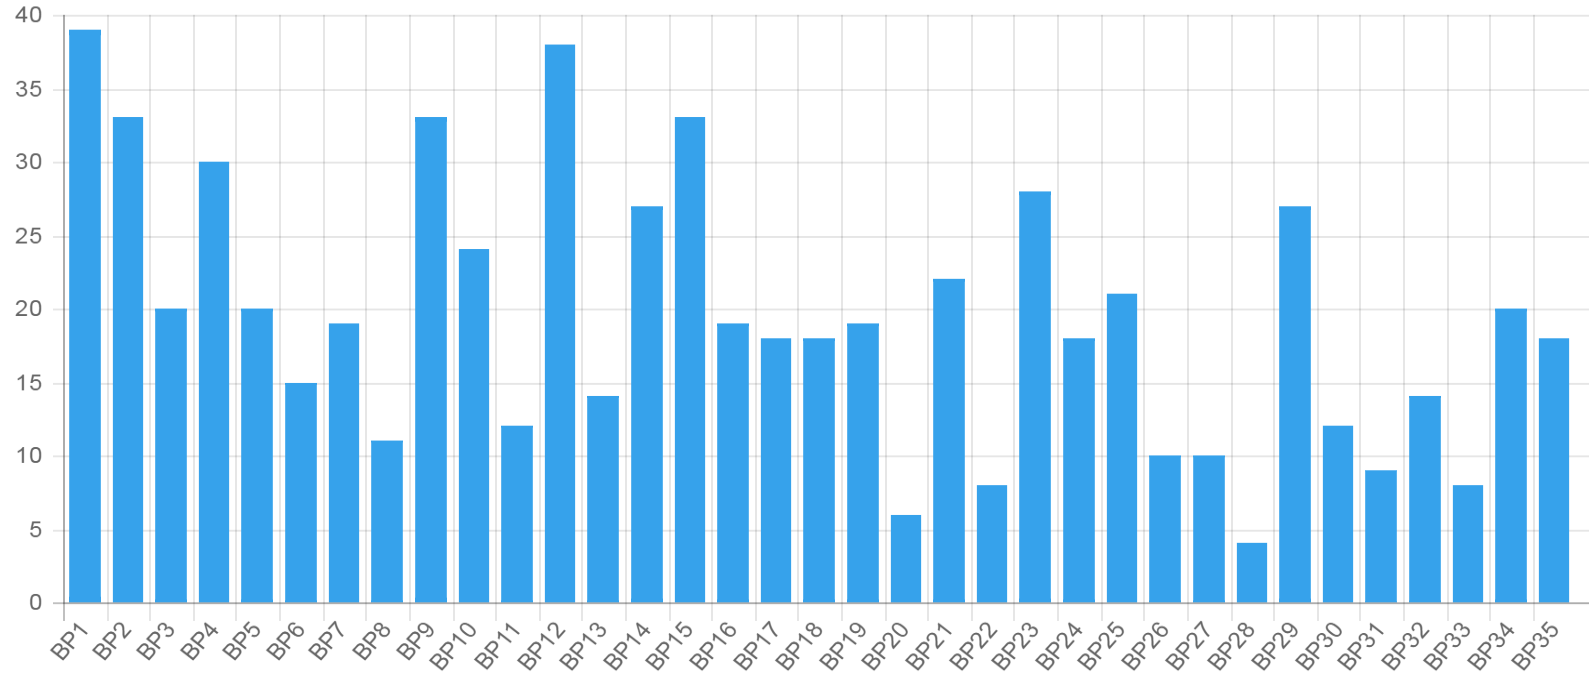
\includegraphics[width=\textwidth]{images/DwbpEvidence.png}
  \caption{DWBP Evidence: Number of candidates implementing a given best practice. \cite{dwbpimplrep}}
  \label{fig:evaldwbpevience}
\end{figure}

\begin{figure}[!htbp]
\centering
  \includegraphics[width=12cm]{images/evalDWBP.png}
  \caption{DWBP Implementation Report Summary: Candidates with number of practices implemented.}
  \label{fig:evaldwbpdatasets}
\end{figure}

\pagebreak
\subsection{The FAIR Data Principles} 
\label{sec:evalfair}

As in the previous section, I want to evaluate \dbpedia with its \dataid metadata against this collection of principles. In this case, I want to find out if \dbpedia offers not only Linked Open Data but if this data is also \textbf{FAIR} (cf. \Cref{sec:fair}). 

\begin{enumerate}
\item[\textbf{F}] \textbf{To be Findable:}
\begin{enumerate}[1]
\item (meta)data are assigned a globally unique and persistent identifier
\begin{flushright}\dataid \& \dbpedia provide unique identifiers \textbf{\color{ForestGreen}(2)}\end{flushright}
\item data are described with rich metadata (defined by R1 below)
\begin{flushright}\dbpedia provides rich metadata with \dataid \textbf{\color{ForestGreen}(2)}\end{flushright}
\item metadata clearly and explicitly include the identifier of the data it describes
\begin{flushright}\dataid includes the identifiers of datasets \textbf{\color{ForestGreen}(2)}\end{flushright}
\item (meta)data are registered or indexed in a searchable resource
\begin{flushright}\dbpedia provides the official \dbpedia SPARQL endpoint \textbf{\color{BurntOrange}(1)}\end{flushright}
\end{enumerate}
\item[\textbf{A}] \textbf{To be Accessible:}
\begin{enumerate}[1]
\item (meta)data are retrievable by their identifier using a standardized communications protocol
\begin{enumerate}
\item the protocol is open, free, and universally implementable
\item the protocol allows for an authentication and authorization procedure, where necessary
\end{enumerate}
\begin{flushright}
the official \dbpedia SPARQL endpoint supports these requirements \textbf{\color{BurntOrange}(1)}
\end{flushright}
\item metadata are accessible, even when the data are no longer available
\begin{flushright}
\dataid documents will remain available \textbf{\color{ForestGreen}(2)}
\end{flushright}
\end{enumerate}
\item[\textbf{I}] \textbf{To be Interoperable:}
\begin{enumerate}[1]
\item (meta)data use a formal, accessible, shared, and broadly applicable language for knowledge representation.
\begin{flushright} (Meta)data is RDF based on well-documented ontologies in both cases. \textbf{\color{ForestGreen}(2)}\end{flushright}
\item (meta)data use vocabularies that follow FAIR principles
\begin{flushright} The \dbpedia ontology and \core allow for FAIR principles. \textbf{\color{ForestGreen}(2)}\end{flushright}
\item (meta)data include qualified references to other (meta)data
\begin{flushright} This is especially true for both \dbpedia data and \dataid{}s. \textbf{\color{ForestGreen}(2)}\end{flushright}
\end{enumerate}
\item[\textbf{R}] \textbf{To be Reusable:}
\begin{enumerate}[1]
\item (meta)data are richly described with a plurality of relevant attributes
\begin{flushright} True for data and metadata. \textbf{\color{ForestGreen}(2)}\end{flushright}
\item (meta)data are released with a clear and accessible data usage license
\begin{flushright} True for data and metadata. \textbf{\color{ForestGreen}(2)}\end{flushright}
\item (meta)data are associated with detailed provenance
\begin{flushright} \dbpedia provides provenance on triple level (in the query of the graph URI), while \dataid{}s of \dbpedia provide origin relations and qualified agent relations (both can be improved) \textbf{\color{BurntOrange}(1)}\end{flushright}
\item (meta)data meet domain-relevant community standards
\begin{flushright} True for data and metadata. \textbf{\color{ForestGreen}(2)}\end{flushright}
\end{enumerate}
\end{enumerate}
The \dbpedia datasets released together with pertaining \dataid{}s prove to be in an excellent FAIR condition, ensuring findability, accessibility, Interoperability and reusability. The underlying prerequisite of these principles (i.e. machine-readability) is also targeted by the general approach of \dataid. According to the FORCE11\footnoteurl{https://www.force11.org} web page about the FAIR principles, \dbpedia releases can be classified as 'FAIR data with open access': "The metadata as well as the data elements themselves are fully FAIR and completely public, under well-defined license."\footnoteurl{https://www.force11.org/fairprinciples} This is equivalent to the fourth (and last) level in their ranking of 'increasingly FAIR digital objects' (cf. \Cref{sec:fair}).


\dataid seems to be a very capable metadata format to assist in the effort of releasing FAIR data.


\pagebreak
\section{Evaluating DataID as dataset metadata} 
\label{sec:evaldataid}

This section offers an evaluation of \dataid (and in particular \core) against multiple possible gauges. This approach will ensure an evaluation of \dataid from the perspective of different communities with their requirements and circumstances.

As in the previous section, requirements can be met in full \textbf{(2)}, partially \textbf{(1)} or not at all \textbf{(0)}. These ratings describe the ability of a vocabulary to fulfil a requirement and not an actual use case.

\subsection{Comparison of DataID core and DCAT}
\label{sec:evaldataid}
In this section, I want to extrapolate a general adequacy of \dataid metadata, from results of the last section, regarding the best practices reviewed.

\Cref{tab:evaldataid} singles out any best practice of the last section for which dataset metadata is a requirement, or it has a direct influence on the expected results. The  compliance of these practices by \core will be compared to the compliance of metadata recorded based solely on the \dcat vocabulary. 

Note: I have taken the liberty to curtail the language of some listed practices. Due to the lack of space, I also shortened \core to \dataid in the heading of the table. Also, while my decisions for each rating for core can be found in the previous section, in the case of \dcat this is not the case. \Cref{sec:dcat} discusses the shortcomings of \dcat in length, a reiteration in this chapter is not necessary.

I conclude that \core offers significant improvements, compared to \dcat, regarding Provenance, Licensing, Access, machine-readability, reusability and Interoperability. Further, a general increase in the richness of describable features is evident, aiding, for example, to describe citations, structural metadata, versioning and coverage.
I grant that multiple aspects still need further improvement (e.g. data quality description or specific properties for deprecated data etc.). \core is a general approach for dataset metadata by design. Its ability to extend easily (cf. \Cref{chap:dmp}) and the explicit context in which to do so (the \ecosystem), provides all necessary means to cover those requirements in a simply achieved extension.

\begin{table}[!htbp]
    \centering
    \begin{tabular}{l|l|l|l}
        \hline
        Ref. & Best Practice & \dataid & \dcat\\
        \hline
        \multicolumn{4}{c}{\textbf{Data on the Web Best Practices}} \\
        \hline
        1 & Provide metadata & \textbf{\color{ForestGreen}(2)} & \textbf{\color{ForestGreen}(2)}\\
        2 & Provide descriptive metadata & \textbf{\color{ForestGreen}(2)} & \textbf{\color{ForestGreen}(2)}\\
        3 & Provide structural metadata & \textbf{\color{ForestGreen}(2)} & \textbf{\color{BurntOrange}(1)}\\
        4 & Provide data license information & \textbf{\color{ForestGreen}(2)} & \textbf{\color{BurntOrange}(1)}\\
        5 & Provide data provenance information & \textbf{\color{ForestGreen}(2)} & \textbf{\color{Mahogany}(0)}\\
        6 & Provide data quality information & \textbf{\color{Mahogany}(0)} & \textbf{\color{Mahogany}(0)}\\
        7 & Provide a version indicator & \textbf{\color{ForestGreen}(2)} & \textbf{\color{ForestGreen}(2)}\\
        8 & Provide a version history & \textbf{\color{BurntOrange}(1)} & \textbf{\color{BurntOrange}(1)}\\
        9 & Use persistent URIs as identifiers of datasets & \textbf{\color{ForestGreen}(2)} & \textbf{\color{ForestGreen}(2)}\\
        12 & Use machine-readable standardized data formats & \textbf{\color{ForestGreen}(2)} & \textbf{\color{BurntOrange}(1)}\\
        13 & Use locale-neutral data representations & \textbf{\color{BurntOrange}(1)} & \textbf{\color{BurntOrange}(1)}\\
        15 & Reuse vocabularies, preferably standardized ones & \textbf{\color{ForestGreen}(2)} & \textbf{\color{ForestGreen}(2)}\\
        22 & Provide an explanation for data that is not available & \textbf{\color{BurntOrange}(1)} & \textbf{\color{BurntOrange}(1)}\\
        28 & Assess dataset coverage & \textbf{\color{ForestGreen}(2)} & \textbf{\color{BurntOrange}(1)}\\
        35 & Cite the Original Publication & \textbf{\color{ForestGreen}(2)} & \textbf{\color{BurntOrange}(1)}\\
        \hline
        \multicolumn{4}{c}{\textbf{FAIR Data Principles}} \\
        \hline
        F1 & globally unique and persistent identifier & \textbf{\color{ForestGreen}(2)} & \textbf{\color{ForestGreen}(2)}\\
        F3 & explicitly includes the identifier of data described & \textbf{\color{ForestGreen}(2)} & \textbf{\color{BurntOrange}(1)}\\
        I1 & uses formal, accessible, shared, applicable language & \textbf{\color{ForestGreen}(2)} & \textbf{\color{ForestGreen}(2)}\\
        I2 & uses vocabularies that follow FAIR principles & \textbf{\color{ForestGreen}(2)} & \textbf{\color{ForestGreen}(2)}\\
        I3 & includes qualified references to other metadata & \textbf{\color{ForestGreen}(2)} & \textbf{\color{Mahogany}(0)}\\
        R1 & is described with a plurality of relevant attributes & \textbf{\color{ForestGreen}(2)} & \textbf{\color{BurntOrange}(1)}\\
        R3 & is associated with detailed provenance & \textbf{\color{ForestGreen}(2)} & \textbf{\color{Mahogany}(0)}\\
        R4 & meets domain-relevant community standards & \textbf{\color{ForestGreen}(2)} & \textbf{\color{ForestGreen}(2)}
    \end{tabular}
    \caption{Comparison of \core and \dcat against metadata relevant best practices of DWBP and FAIR}
    \label{tab:evaldataid}
\end{table}

\subsection{Comparing DataID to a host of vocabularies}
\label{sec:evalvocabularies}

I want to go a pace further and compare \core to every vocabulary discussed in \Cref{sec:dv}, as well as some of their combinations. This will provide a clearer picture of what has been accomplished with this work. 

While the means of evaluation in the previous section, based on the principles discussed before, is a useful tool for comparing vocabularies, it is not sufficient. Important aspects of dataset metadata are not reflected in the best practices (such as reflection on Extensibility and Interoperability). Therefore, I will use the principle goals of dataset metadata, which I introduced in \Cref{sec:dv}, to evaluate \core against other metadata vocabularies.

\begin{enumerate}[A]
\item \textbf{The vocabulary encourages the use of richly described and machine-readable resources.} This is one of the underlying objectives of \dataid; to provide machine-readable resources where possible (cf. \Cref{sec:objectives}). 
\hfill\textbf{\color{ForestGreen}(2)}
\item \textbf{The vocabulary assigns globally unique URIs to metadata resources.}
That is a given for every RDF-based vocabulary. 
\hfill\textbf{\color{ForestGreen}(2)}
\item \textbf{The vocabulary can describe data access and access restrictions, consumable for humans and machines alike.} \core provides detailed descriptions of media types \prop{dataid:MediaType} and other related aspects (e.g. access procedures). Additional effort is needed to describe, for example, API endpoints. Extensions for such a purpose is subject to future work.
\hfill\textbf{\color{BurntOrange}(1)}
\item \textbf{The vocabulary can portray provenance information extensively.}
\prov is imported into \core and additional qualifications were created (such as \prop{dataid:Authorization}.
\hfill\textbf{\color{ForestGreen}(2)}
\item \textbf{The vocabulary provides for detailed descriptions of rights and licenses.}
Licenses and other policies can be described in detail with \prop{odrl:Policy}.
\hfill\textbf{\color{ForestGreen}(2)}
\item \textbf{The vocabulary provides properties to cite identifiers of the data described.}
This is achievable with axioms of the \prov ontology. The \textit{Activities \& Plans} extension of \dataid offers the class \prop{dataid-acp:SupportingEntity} which (with its sub-classes) can further delimit such entities.
\hfill\textbf{\color{BurntOrange}(1)}
\item \textbf{The vocabulary provides for qualified references between resources.}
In addition to the natural qualifying mechanisms of \prov, \core provides for further qualifications for related Agents and Datasets. 
\hfill\textbf{\color{ForestGreen}(2)}
\item \textbf{The vocabulary is easy to extend, to fit any given use case.}
This feature was demonstrated with \Cref{chap:dmp} of this thesis.
\hfill\textbf{\color{ForestGreen}(2)}
\item \textbf{The vocabulary is unambiguous and easy to map to other metadata vocabularies.}
\core does not impede the Extensibility of \dcat and is therefore easy to map to other vocabularies (cf. \Cref{chap:map}).
\hfill\textbf{\color{ForestGreen}(2)}
\item \textbf{The vocabulary offers additional properties to aid dissemination and discovery.}
Multiple properties have been introduced for Datasets to further describe its intended purpose and other useful information, applicable to dissemination tasks.
\hfill\textbf{\color{ForestGreen}(2)}
\end{enumerate}

This table includes all evaluations of that kind from \Cref{sec:dv}, compared to \core. I also included some amalgamation between \dcat and other ontologies to demonstrate how metadata based on such an approach would fare.
This rather crude method of gauging the quality of a vocabulary is of cause plagued with inadequacies, but it reflects the broader aspects of the \dataid approach compared to other dataset metadata in an assessable manner. 

\begin{table}[!htbp]
    \centering
    \begin{tabular}{|l|l|l|l|l|l|l|l|l|l|l|l|}
        \hline
        Vocabulary & A & B & C & D & E & F & G & H & I & J & Sum \\
        \hline
        \dcat & 1 & 2 & 1 & 0 & 0 & 1 & 0 & 2 & 2 & 1 & 10 \\
        \void & 1 & 2 & 0 & 0 & 0 & 0 & 1 & 1 & 2 & 1 & 8 \\
        \ckan & 0 & 2 & 0 & 0 & 0 & 0 & 0 & 1 & 1 & 0 & 4 \\
        \metashare & 2 & 2 & 1 & 1 & 2 & 0 & 0 & 0 & 1 & 1 & 10 \\
        \adms & 1 & 2 & 1 & 0 & 0 & 1 & 0 & 2 & 2 & 1 & 10 \\
        \dcatap & 1 & 2 & 1 & 0 & 0 & 1 & 0 & 1 & 2 & 1 & 9 \\
        HCLS Profile & 2 & 2 & 2 & 1 & 0 & 1 & 0 & 2 & 1 & 1 & 12 \\
        \cerif & 2 & 2 & 1 & 1 & 0 & 2 & 2 & 2 & 2 & 1 & 15 \\
        \cmdi & 1 & 2 & 0 & 0 & 1 & 2 & 0 & 2 & 0 & 1 & 9 \\
        \dataid 1.0.0 & 1 & 2 & 1 & 1 & 2 & 1 & 2 & 1 & 2 & 1 & 14 \\
        \hline
        \dcat \& \prov & 1 & 2 & 1 & 1 & 0 & 1 & 2 & 2 & 2 & 1 & 13 \\ 
        \dcat \& \void & 1 & 2 & 1 & 0 & 0 & 1 & 1 & 2 & 2 & 1 & 11 \\
        \dcat \& \prov \& \void & 1 & 2 & 1 & 1 & 0 & 1 & 2 & 2 & 2 & 1 & 13 \\
        \hline
        \core & 2 & 2 & 1 & 2 & 2 & 1 & 2 & 2 & 2 & 2 & 18 \\
        \hline
    \end{tabular}
    \caption{Comparison of dataset vocabularies introduced in \Cref{sec:dv} to \core}
    \label{tab:evaldcat}
\end{table}

As the table indicates, \dataid has made some strides to cover aspects of dataset metadata, which are inadequately represented or neglected altogether by other metadata formats. Especially aspects such as the representation of Licensing, Provenance, machine-readability, Access, discoverability, Extensibility and Interoperability were accomplished.

\pagebreak
\subsection{Implementation of Objectives}
\label{sec:evalimplementation}
\textit{Improving the portrayal of Provenance, Licensing and Access, while maintaining the easy Extensibility and Interoperability of \dcat, are the linchpin objectives in my effort to present a comprehensive, extensible and interoperable metadata vocabulary} (cf. \Cref{sec:objectives}).

With the evidence already gathered in this section, I want to assess the fulfilment of those goals set for \dataid in \Cref{sec:objectives}. I will list all possible proof for accomplishing each objective as a foundation for a final judgement of success.

\paragraph{Objective 1.} Provide sufficient support for extensive and machine-readable representations for Provenance, Licensing and data Access.

Beginning with the very first version of \dataid, Provenance was one of the topmost items on my list to improve dataset metadata, as an omnipresent requirement in most use cases with large or complex datasets. With the conception of the Provenance Ontology (\prov) and its characteristic way of representation and interchange of provenance information on the Web, the ideal companion ontology for \dcat was found. By creating the means to qualify relations, (re-) introducing the effective approach of inserting relationship objects as mediators between subject and object, relationships can express roles, temporal or spatial restrictions and experience state changes. This measure ensures the referential and functional integrity of the involved Entities.
\todo{talk about referential integrity}

In addition to the basic possibility to qualify relations between Entities, Agents and Activities, \core specialised in particular on relations between (dataset) Entities and Agents. With \prop{dataid:Authorization} a qualification object for such relations was introduced, providing a record about what an Agent is allowed to do with a particular collection of Entities. The \prop{dataid:DatasetRelationship} mediator between different datasets allows for a well-defined possibility to declare any relation, two datasets might enter into. 
Currently, the \ecosystem provides the extension \textit{Activities \& Plans}, which further specifies ways to record Provenance, focusing on Activities and Plans. Its applicability was demonstrated in \Cref{chap:dmp}.

The better portrayal of Licensing information was accomplished by the adoption of the \odrl ontology to represent any policy or license agreement. \odrl descriptions provide a flexible and interoperable mechanisms to support the  transparent use of digital content in publishing, distribution, and consumption of digital media in a machine-readable way. Restricting the range of \prop{dct:license} to instances of \prop{odrl:Policy}, ensuring the use of machine-readable licenses, offers a way to automatically decide if a dataset is admissible in the context of a particular transformation activity.

Various efforts have been made to support a sustainable mode of Access to the digital objects described in a \dataid document. The initial idea of separating Datasets as a concept and their possible manifestations in Distributions was a significant improvement of the \dcat vocabulary to previous representations. Alas, \dcat is too generic, which leaves too much room for interpretation and ambiguity.

To alleviate this lack of specificity, I implemented the \prop{dataid:MediaType} class, to define the type of a digital object in a machine-readable way. Multiple sub-classes of \prop{dataid:Distribution} offers an interface for further specification (e.g. for API endpoints). Additional properties (such as \prop{dataid:checksum} aid the acquisition of data in an automatic processing environment.

\paragraph{Objective 2.} Extend \dcat with well-established ontologies to resolve the pressing issues with dataset metadata if possible

Throughout the \ecosystem, I tried to reuse existing ontologies which are either well-establish in the Semantic Web community (preferably W3C recommended), or innovative and of sufficient maturity to contribute its semantics to \dataid.
This table shows the result of this effort. Each reused ontology from the \ecosystem is recorded here, together with its origin and a statement about its maturity. Those ontologies used in \core are marked with an asterisk.
%\footnote{Note: Ontology marked with an * are imported into \core, while a + mark, denotes that an ontology is reused only}.

\begin{table}[!htbp]
    \centering
    \begin{tabular}{|l|l|l|}
        \hline
        Ontology & Origin & Maturity \\
        \hline
        Dublin Core* & DCMI Initiative & deemed a Good Ontology (W3C)\\
        \dcat* & W3C Working Group & W3C recommended\\
        \prov* & W3C Working Group & W3C recommended\\
        \void* & W3C Interest Group & W3C Interest Group specification\\
        \foaf* & The FOAF project & deemed a Good Ontology (W3C)\\
        DataCite* & DataCite & Part of the SPAR ontology suite\\
        \dlo & ALIGNED project & parallel developed with \dataid\\
        \lvont* & Lexvo.org & widely used ontology through-\\
        & & out the NLP community\\
        \odrl* & W3C Community Group & final specification\\
        \org & W3C Working Group & W3C recommended\\
        \sd & W3C Working Group & W3C recommended\\
        \spdx* & Linux Foundation & specification\\
        \hline
    \end{tabular}
    \caption{All external vocabularies reused by ontologies of the \ecosystem}
    \label{tab:evalontos}
\end{table}

\core only imports recommended or otherwise supported ontologies by the W3C.
\todo{datacite?}
Ontologies, such as \lvont, \odrl and \spdx are used to restrict some property ranges but are not imported, as to keep a separation between \dataid and developments of the origin environment of these ontologies.

\paragraph{Objective 3.} Show, that by modularising into a landscape of ontologies, \dataid preserves the general character of \dcat, supporting Extensibility and Interoperability.

As discussed in \Cref{sec:multilayer}, to keep \dataid as extensible and interoperable as \dcat, I decided to modularize \dataid into multiple extension ontologies around a single core. 

The modular approach paired with the effort to keep \core as general (simplistic) as possible, without compromising on the goals lined out, has proven to be an expedient solution. As a side effect, \core adheres to profile OWL2 RL\footnote{with the exception of the 5 axioms of the \prov ontology pointed out in the \prov specification: \url{https://www.w3.org/TR/prov-o/#owl-profile}} 
\todo{put this somewhere not in a footnote} 
which adds additional possibilities to use cases where reasoning over metadata is of concern and simplifies the extending of this ontology.

Modularity and simplicity are general aspects of good metadata (cf. \Cref{sec:metadata}) and can be seen as the foundation for subsequent traits such as Extensibility and Interoperability. Both of these characteristics were demonstrated in \Cref{chap:dmp} and \Cref{chap:map} respectively. With these measures in place, \core extends \dcat in a way, which does not impede its wide applicability in data portals and other applications. Existing \dcat solutions can therefore easily be transformed into \dataid based metadata. 

\paragraph{Objective 4.} Prove that the resulting ecosystem is capable of serving for complex demands on dataset metadata (proving Extensibility).

I exemplified the implementation of specialised dataset metadata vocabularies extending \core in \Cref{chap:dmp}. Based on workflow for publishing \dataid metadata parallel to its datasets in \Cref{chap:bestprctice}. I have shown that by extending \core with existing addendums and even external ontologies, one could satisfy complex metadata requirements like those of Data Management Plans while keeping the ability to inter-operate with other metadata vocabularies (like \cmdi - cf. \Cref{chap:map}) in turn.

\paragraph{Objective 5.} Demonstrate the Interoperability with other metadata formats.

Exchanging information between systems using different metadata schemas is an important aspect in any such scenario. I have shown in \Cref{chap:map} how \dataid is supporting the Interoperability of its metadata. 

\begin{itemize}
\item By basing \dataid on \dcat, a well established and often used vocabulary for dataset metadata offering the easiest form of Interoperability: agreement on a schema.
\item By modularising \dataid, easing mapping efforts by reducing ambiguity. 
\item By allowing for extensions which could either incorporate the other vocabulary altogether or accommodate any missing expressiveness with a special extension.
\end{itemize}

\paragraph{Objective 6.} Evaluate the universal applicability of \dataid for datasets against common demands on data publications.

While objectives 1. to 5. represented the principle goals for \dataid, there are other important demands on dataset metadata which \dataid can serve. Most of these demands are already mentioned in \Cref{sec:evaldataid}. I will single out the more salient aspects.

\begin{itemize}
\item \textbf{Machine-readability} - \dataid tries to be as specific as possible. For example, replacing simple literals with \prop{dataid:SimpleStatement} or other concepts suitable for the property at hand.
\item \textbf{Versioning} - \dataid introduced simple (but effective) version pointers between dataset Entities.
\item \textbf{Identifiers} - by adopting the identifier concept of the DataCite ontology, \core provides a comprehensive means to specify (alternative) identifiers, for any digital object.
\item \textbf{Dissemination} - the Dataset concept of \core provides multiple textual statements for publishers to record intent, purpose or possible usefulness of datasets, all of which are helpful for dissemination tasks and general discoverability.
\item \textbf{Rights \& Responsibilities} - \dataid offers a prominent feature to not only define roles an Agent might have regarding an Entity but also what kind of responsibilities and rights this entails.
Exact definitions of authorisations in the context of datasets become feasible.
\end{itemize}

In summary, \dataid does not only fulfil the objectives set but extends a wide range of useful additions to the core model established by \dcat. 

\subsection{Conformity to the ALIGNED principles}
\label{sec:evalaligned}

In the context of the ALIGNED project, \dataid is part of a shared model of software and data engineering to enable unified governance and coordination between aligned co-evolving software and data lifecycles.
I want to confirm that the overall approach of \dataid does comply with the three principles of ALIGNED, which were set up to guide all relevant tasks:

\paragraph{To be part of a unified software and data engineering process;}
With the incorporation of the Data Lifecycle Ontology of the ALIGNED project (cf. \Cref{sec:dmpmodel}) into the \textit{Activities \& Plans} extension of \dataid, I combined both ontologies of the Data Management side of the ALIGNED Suite of Ontologies \cite{SolankiBFKDB16}, specifically designed to model the information exchange needs of combined software and data engineering.

\paragraph{describing the complete data lifecycle and domain model;}
Both ontologies can jointly describe a domain data model in the context of a progressing data lifecycle and provide the necessary artefacts to aid the software lifecycle advancing in parallel.

\paragraph{with an emphasis on quality, productivity and agility.}
Rich metadata of datasets will increase the quality of any dependent process and its results. The ability to adapt easily to a given use case and its high level of Interoperability provides sufficient flexibility for agile engineering processes. The focus on machine-readability and detailed descriptions of resources is an excellent basis for a high degree of automation in data engineering workflows.

The \dataid project started out solely as a tool to publish \dbpedia datasets with more descriptive metadata. With the start of the ALIGNED project, which uses \dbpedia as one of its use cases, \dataid has been included in the ALIGNED suite of ontologies that provide semantic models of design intents, domain-specific datasets, software engineering processes, quality heuristics and error handling mechanisms \cite{SolankiBFKDB16}.  The suite contributes immensely towards enabling Interoperability and alleviating some of the complexities involved.

Combining data and software engineering processes to increase quality, productivity and agility, is a challenge being faced by several organisations aiming to exploit the benefits of Big Data. Ontologies and vocabularies developed in accordance with competency questions, objective criteria and ontology engineering principles can provide useful support to data scientists and software engineers undertaking the challenge. 
%As ontologies from the suite are now in various stages of adoption by the ALIGNED use cases, the next steps would incorporate their empirical evaluation.

\chapter{Conclusion and Future Work}
\label{chap:future}

This work presented a comprehensive introduction to \dataid, providing structured dataset metadata for any domain, type of data or dataset structure. In particular, \core was portrayed in great detail as the kernel element of the \ecosystem. 

Based on a study of existing metadata vocabularies, an extensive list of inadequacies and further demands on dataset metadata was compiled, guiding the course of this work.
As a result, the monolithic approach of a first version of the \dataid ontology was modularised into multiple extension ontologies around a single core.
\core extends the \dcat vocabulary to provide greater specificity on many important issues (such as Access, Licensing and Provenance), without encroaching on the central traits of \dcat, easy Extensibility and Interoperability with other existing dataset metadata formats. 
Furthermore, this thesis demonstrated the abilities of the \ecosystem to accommodate for complex metadata requirements (i.e. Data Management Plans), by extending \core and even incorporating external ontologies (i.e. \redata ontology), while keeping the ability to interoperate with other metadata vocabularies (such as \cmdi) in turn.
Its ability to model complex authorisations with minimal effort for any dataset environment offers additional possibilities for comprehensive metadata demands.
%It serves as a controlled environment in which to extend \core with existing extensions and use case specific adaptations

\dataid metadata has proven to be a very promising partner for dataset publishers, such as \dbpedia, aiding not only publication tasks, but providing the comprehensive metadata needed to align with the best practices of FAIR and the Data on the Web W3C working group.
Moreover, \dataid has shown that it is capable of serving as a pivotal member in the ALIGNED Suite of Ontologies to cover all demands for dataset metadata in the context of the co-evolving lifecycles of software and data management.

In total, \core consists of 19 classes, 43 object properties, eight datatype properties and 29 named individuals. It is consistent with the OWL2 RL profile (with minor adaptations, see \Cref{}).
\todo{todo} 
The \ecosystem provides a controlled environment, in which the interplay of different extensions and \core is regulated and documented, making it easy to combine multiple extensions with \core to solve a given usage scenario. Currently, \core can be extended by three existing extensions from the common layer of the \ecosystem, with more already planned.

Additional work has to be done in defining the proper inter-semantics of the \ecosystem.
In that, appropriate regulations and guidelines have to be in place before incorporating new \dataid extensions into the common layer of ontologies. A toolchain for validating the interoperability of multiple extensions in one ontology would go a long way in helping users to compile their use case extensions. I have suggested the Dacura Data Curation System\footnoteurl{http://dacura.cs.tcd.ie} as a possible solution.

Currently, a \dataid service stack and website is being implemented, to simplify and automate the creation, validation and dissemination of \dataid{}s, supporting humans in creating \dataid{}s manually, as well as automation tasks with a service endpoint. Multiple \dataid related tasks will be usable for humans and machines:

\begin{itemize}
\item support for the creation of dataset metadata, guiding the user through all necessary steps in creating a \dataid
\item providing help when selecting the right combination of \dataid extensions to solve a particular use case
\item validation of newly created \dataid{}s or any other \dataid document with a website or directly through a service endpoint
\item automatic publication of \dataid documents to dataset portals like Datahub\footnoteurl{https://datahub.io} or Linghub\footnoteurl{http://linghub.lider-project.eu}
\end{itemize}

Integrating \dataid fully into the processes and tools defined by the ALIGNED project is another outstanding task.


%************************************************************************************************************************
%* glossary, appendix, bibliography, etc.
%************************************************************************************************************************

\addchap{Glossary}   
\begin{description}
\item[Vocabulary] On the Semantic Web, vocabularies define the concepts and relationships (also referred to as "terms") used to describe and represent an area of concern. Vocabularies are used to classify the terms that can be used in a particular application, characterize possible relationships, and define possible constraints on using those terms. In practice, vocabularies can be very complex (with several thousands of terms) or very simple (describing one or two concepts only)\cite{W3CVOCONTO}.

\item[Ontology] There is no clear division between what is referred to as "vocabularies" (cf. Vocabulary) and "ontologies". The trend is to use the word "ontology" for more complex, and possibly quite formal collection of terms, whereas "vocabulary" is used when such strict formalism is not necessarily used or only in a very loose sense. Vocabularies are the basic building blocks for inference techniques on the Semantic Web\cite{W3CVOCONTO}.

\item[Application Profile] a set of metadata elements defined for a particular application or other limited purposes, often based on a broader schema (like an ontology). Such a profile is either constructed under a closed world assumption or provides many restrictions to create a view \todo{go on}

\item[AP-NISO]Profiles are subsets of a scheme
that are implemented by a particular
interest group. Profiles can
constrain the number of elements
that will be used, refine element
definitions to describe the specific
types of resources more accurately,
and specify values that an element
can take.

\item[Extension] An extension is the
addition of elements to an
already developed
scheme to support the
description of an information
resource of a
particular type or subject
or to meet the needs of a
particular interest group.
Extensions increase the
number of elements.

\item[Entity–relationship model] describes inter-related things of interest in a specific domain of knowledge. An ER model is composed of entity types (which classify the things of interest) and specifies relationships that can exist between instances of those entity types.
\end{description}

%\bibliographystyle{alpha}
%\bibliography{own.bib}
\printbibliography[title=References]

\addchap{Appendix I}
\label{chap:appendix1}

\paragraph{DataID core specification}

This work will not include the whole specification of \core.
Instead I provide the revision number at the time of writing of the ontology specification file (dataid.ttl):

\textbf{bbdacd50dd6389bc435a576a03753c7101a6ac02}\footnoteurl{https://github.com/dbpedia/DataId-Ontology/commit/bbdacd50dd6389bc435a576a03753c7101a6ac02}
\\\\
The latest version of this specification is always available under the namespace URI of \dataid:

\textbf{\url{http://dataid.dbpedia.org/ns/core.ttl}}

\addchap{Appendix II}
\label{chap:appendix2}
\begin{lstlisting}[language=ttl, captionpos=b, label=lst:dcex,linewidth=\columnwidth,breaklines=true,basicstyle=\ttfamily\scriptsize]
@prefix dataid: <http://dataid.dbpedia.org/ns/core#> .
@prefix dataid-ld: <http://dataid.dbpedia.org/ns/ld#> .
@prefix dataid-mt: <http://dataid.dbpedia.org/ns/mt#> .
@prefix dcat:  <http://www.w3.org/ns/dcat#> .
@prefix datacite: <http://purl.org/spar/datacite/> .
@prefix void:  <http://rdfs.org/ns/void#> .
@prefix spdx:  <http://spdx.org/rdf/terms#> .
@prefix owl:   <http://www.w3.org/2002/07/owl#> .
@prefix rdfs:  <http://www.w3.org/2000/01/rdf-schema#> .
@prefix prov:  <http://www.w3.org/ns/prov#> .
@prefix foaf:  <http://xmlns.com/foaf/0.1/> .
@prefix dct:    <http://purl.org/dc/terms/> .
@prefix sd:    <http://www.w3.org/ns/sparql-service-description#> .
@base <http://downloads.dbpedia.org/2015-10/core-i18n/ar/2015-10_> .

<dataid_ar.ttl>
        a                          dataid:DataId ;
        dataid:associatedAgent     <http://wiki.dbpedia.org/dbpedia-association> , <http://wiki.dbpedia.org/dbpedia-association/persons/Freudenberg> ;
        dataid:inCatalog           <http://downloads.dbpedia.org/2015-10/2015-10_dataid_catalog.ttl> ;
        dataid:latestVersion       <http://downloads.dbpedia.org/2016-04/core-i18n/ar/2016-04_dataid_ar.ttl> ;
        dataid:nextVersion         <http://downloads.dbpedia.org/2016-04/core-i18n/ar/2016-04_dataid_ar.ttl> ;
    	dataid:previousVersion     <http://downloads.dbpedia.org/2015-04/core-i18n/ar/2015-04_dataid_ar.ttl> ;
        dataid:underAuthorization  <dataid_ar.ttl?auth=maintainerAuthorization> , <dataid_ar.ttl?auth=creatorAuthorization> ;
        dct:hasVersion              <dataid_ar.ttl?version=1.0.0> ;
        dct:issued                  "2016-08-02"^^xsd:date ;
        dct:modified                "2016-10-13"^^xsd:date ;
        dct:publisher               <http://wiki.dbpedia.org/dbpedia-association> ;
        dct:title                   "DataID metadata for the Arabic DBpedia"@en ;
        foaf:primaryTopic          <dataid_ar.ttl?set=maindataset> .

#### Agents & Authorizations ####

<http://wiki.dbpedia.org/dbpedia-association/persons/Freudenberg>
        a                        dataid:Agent ;
        dataid:hasAuthorization  <dataid_ar.ttl?auth=maintainerAuthorization> ;
        dataid:identifier        <http://www.researcherid.com/rid/L-2180-2016> ;
        foaf:mbox                "freudenberg@informatik.uni-leipzig.de" ;
        foaf:name                "Markus Freudenberg" .
        
<dataid_ar.ttl?auth=maintainerAuthorization>
        a                          dataid:Authorization ;
        dataid:authorityAgentRole  dataid:Maintainer ;
        dataid:authorizedAgent     <http://wiki.dbpedia.org/dbpedia-association/persons/Freudenberg> ;
        dataid:authorizedFor       <dataid_ar.ttl> ;
        dataid:isInheritable       true .

<http://www.researcherid.com/rid/L-2180-2016>
        a                              dataid:Identifier ;
        dataid:literal                  "L-2180-2016" ;
        dct:issued                      "2016-08-01"^^xsd:date ;
        dct:references                  <http://www.researcherid.com/rid/L-2180-2016> ;
        datacite:usesIdentifierScheme  datacite:researcherid .

<http://wiki.dbpedia.org/dbpedia-association>
        a                        dataid:Agent ;
        dataid:hasAuthorization  <dataid_ar.ttl?auth=creatorAuthorization> ;
        foaf:homepage            <http://dbpedia.org> ;
        foaf:mbox                "dbpedia@infai.org" ;
        foaf:name                "DBpedia Association" .

<dataid_ar.ttl?auth=creatorAuthorization>
        a                          dataid:Authorization ;
        dataid:authorityAgentRole  dataid:Creator ;
        dataid:authorizedAgent     <http://wiki.dbpedia.org/dbpedia-association> ;
        dataid:authorizedFor       <dataid_ar.ttl> ;
        dataid:isInheritable       true .
        
<https://wikimediafoundation.org>
        a                        dataid:Agent ;
        dataid:hasAuthorization  <http://dbpedia.org/dataset/pages_articles?lang=ar&dbpv=2016-04&file=pages_articles_ar.xml.bz2&auth=publisherAuthorization> , <http://dbpedia.org/dataset/pages_articles?lang=ar&dbpv=2016-04&auth=publisherAuthorization> ;
        foaf:mbox                "info@wikimedia.org" ;
        foaf:name                "Wikimedia Foundation, Inc." .
        
<dataid_ar.ttl?auth=publisherAuthorization>
        a                          dataid:Authorization ;
        dataid:authorityAgentRole  dataid:Creator, dataid:Publisher ;
        dataid:authorizedAgent     <https://wikimediafoundation.org> ;
        dataid:authorizedFor       <dataid_ar.ttl?set=pages_articles> ;
        dataid:isInheritable       true .
        
########## Main Dataset ##########

<dataid_ar.ttl?set=maindataset>
        a                       dataid:Superset ;
        dataid:associatedAgent  <http://wiki.dbpedia.org/dbpedia-association> , <http://wiki.dbpedia.org/dbpedia-association/persons/Freudenberg>  ;
        dataid:growth               <dataid_ar.ttl?stmt=growth> ;
        dataid:openness             <dataid_ar.ttl?stmt=openness> ;
        dataid:reuseAndIntegration  <dataid_ar.ttl?stmt=reuseAndIntegration> ;
        dataid:similarData          <dataid_ar.ttl?stmt=similarData> ;
        dataid:usefulness           <dataid_ar.ttl?stmt=usefulness> ;
        dct:description          """DBpedia is a crowd-sourced community effort to extract structured information from Wikipedia and make this information available on the Web. DBpedia allows you to ask sophisticated queries against Wikipedia, and to link the different data sets on the Web to Wikipedia data. We hope that this work will make it easier for the huge amount of information in Wikipedia to be used in some new interesting ways. Furthermore, it might inspire new mechanisms for navigating, linking, and improving the encyclopedia itself."""@en ;
        dct:hasVersion           <dataid_ar.ttl?version=1.0.0> ;
        dct:issued               "2016-07-02"^^xsd:date ;
        dct:language             <http://lexvo.org/id/iso639-3/ara> ;
        dct:license              <http://purl.oclc.org/NET/rdflicense/cc-by-sa3.0> ;
        dct:modified             "2016-08-01"^^xsd:date ;
        dct:publisher            <http://wiki.dbpedia.org/dbpedia-association> ;
        dct:rights               <dataid_ar.ttl?rights=dbpedia-rights> ;
        dct:title                "DBpedia root dataset for Arabic, version 2015-10"@en ;
        void:subset             <dataid_ar.ttl?set=long_abstracts_en_uris>, <dataid_ar.ttl?set=interlanguage_links> ;
        void:vocabulary         <http://downloads.dbpedia.org/2015-04/dbpedia_2015-10.owl> ;
        dcat:keyword            "maindataset"@en , "DBpedia"@en ;
        dcat:landingPage        <http://dbpedia.org/> ;
        foaf:isPrimaryTopicOf   <dataid_ar.ttl> ;
        foaf:page               <http://wiki.dbpedia.org/Downloads2015-10> .

############ Datasets #############
     
<dataid_ar.ttl?set=interlanguage_links>
        a                       dataid:Dataset, dataid-ld:LinkedDataDataset ;
        rdfs:label              "interlanguage links"@en ;
        dataid:associatedAgent  <http://wiki.dbpedia.org/dbpedia-association> , <http://wiki.dbpedia.org/dbpedia-association/persons/Freudenberg> ;
        dct:description          "Dataset linking a DBpedia resource to the same resource in other languages and in Wikidata."@en ;
        dct:hasVersion           <dataid_ar.ttl?version=1.0> ;
        dct:isPartOf             <dataid_ar.ttl?set=maindataset> ;
        dct:issued               "2016-07-02"^^xsd:date ;
        dct:language             <http://lexvo.org/id/iso639-3/ara> ;
        dct:license              <http://purl.oclc.org/NET/rdflicense/cc-by-sa3.0> ;
        dct:modified             "2016-08-02"^^xsd:date ;
        dct:publisher            <http://wiki.dbpedia.org/dbpedia-association> ;
        dct:title                "interlanguage links"@en ;
        void:rootResource       <dataid_ar.ttl?set=maindataset> ;
        void:triples            7480764 ;
        dcat:distribution       <dataid_ar.ttl?file=interlanguage_links_ar.ttl.bz2> , <dataid_ar.ttl?file=interlanguage_links_ar.tql.bz2> ;
        dcat:keyword            "DBpedia"@en , "interlanguage_links"@en ;
        dcat:landingPage        <http://dbpedia.org/> ;
        sd:defaultGraph         <http://ar.dbpedia.org> ;
        foaf:page               <http://wiki.dbpedia.org/Downloads2015-10> .
        
<dataid_ar.ttl?set=long_abstracts_en_uris>
        a                       dataid:Dataset, dataid-ld:LinkedDataDataset ;
        rdfs:label              "long abstracts en uris"@en ;
        dataid:associatedAgent  <http://wiki.dbpedia.org/dbpedia-association> , <http://wiki.dbpedia.org/dbpedia-association/persons/Freudenberg> ;
        dataid:qualifiedDatasetRelation   <dataid_ar.ttl?relation=source&target=pages_articles> ;
        dataid:relatedDataset   <dataid_ar.ttl?set=pages_articles> ;
        dct:description          "Full abstracts of Wikipedia articles, usually the first section. Normalized resources matching English DBpedia."@en ;
        dct:hasVersion           <dataid_ar.ttl?version=1.0.0> ;
        dct:isPartOf             <dataid_ar.ttl?set=maindataset> ;
        dct:issued               "2016-07-02"^^xsd:date ;
        dct:language             <http://lexvo.org/id/iso639-3/ara> ;
        dct:license              <http://purl.oclc.org/NET/rdflicense/cc-by-sa3.0> ;
        dct:modified             "2016-08-02"^^xsd:date ;
        dct:publisher            <http://wiki.dbpedia.org/dbpedia-association> ;
        dct:title                "long abstracts en uris"@en ;
        void:rootResource       <dataid_ar.ttl?set=maindataset> ;
        void:triples            232801 ;
        void:sparqlEndpoint      <http://dbpedia.org/sparql> ;
        dcat:distribution       <dataid_ar.ttl?sparql=DBpediaSparqlEndpoint> , <dataid_ar.ttl?file=long_abstracts_en_uris_ar.ttl.bz2> , <dataid_ar.ttl?file=long_abstracts_en_uris_ar.tql.bz2> ;
        dcat:keyword            "long_abstracts_en_uris"@en , "DBpedia"@en ;
        dcat:landingPage        <http://dbpedia.org/> ;
        sd:defaultGraph         <http://ar.dbpedia.org> ;
        foaf:page               <http://wiki.dbpedia.org/Downloads2015-10> .
        
<dataid_ar.ttl?set=pages_articles>
        a                          dataid:Dataset ;
        rdfs:label                 "Wikipedia XML source dump file"@en ;
        dataid:associatedAgent     <https://wikimediafoundation.org> ;
        dataid:needsSpecialAuthorization  <dataid_ar.ttl?auth=publisherAuthorization> ;
        dct:description             "The Wikipedia dump file, which is the source for all other extracted datasets."@en ;
        dct:hasVersion              "20160305" ;
        dct:issued                  "2016-03-05"^^xsd:date ;
        dct:language                <http://lexvo.org/id/iso639-3/ara> ;
        dct:license                 <http://purl.oclc.org/NET/rdflicense/cc-by-sa3.0> ;
        dct:publisher               <https://wikimediafoundation.org> ;
        dct:title                   "Wikipedia XML source dump file"@en ;
        dcat:distribution          <http://dbpedia.org/dataset/pages_articles?lang=ar&dbpv=2016-04&file=pages_articles_ar.xml.bz2> ;
        dcat:keyword               "Wikipedia"@en , "XML dump file"@en ;
        dcat:landingPage           <https://meta.wikimedia.org/wiki/Data_dumps> .
        
########## Distributions ###########

<dataid_ar.ttl?file=interlanguage_links_ar.ttl.bz2>
        a                            dataid:SingleFile ;
        rdfs:label                   "interlanguage_links_ar.ttl.bz2" ;
        dataid:associatedAgent       <http://wiki.dbpedia.org/dbpedia-association> , <http://wiki.dbpedia.org/dbpedia-association/persons/Freudenberg> ;
        dataid:checksum              <dataid_ar.ttl?file=interlanguage_links_ar.ttl.bz2&checksum=md5> ;
        dataid:isDistributionOf      <dataid_ar.ttl?set=interlanguage_links> ;
        dataid:preview               <http://downloads.dbpedia.org/preview.php?file=2015-10_sl_core-i18n_sl_ar_sl_interlanguage_links_ar.ttl.bz2> ;
        dataid:uncompressedByteSize  1184687767 ;
        dct:description               "Dataset linking a DBpedia resource to the same resource in other languages and in Wikidata."@en ;
        dct:hasVersion                <dataid_ar.ttl?version=1.0> ;
        dct:issued                   "2016-07-02"^^xsd:date ;
        dct:license                   <http://purl.oclc.org/NET/rdflicense/cc-by-sa3.0> ;
        dct:modified                  "2016-08-02"^^xsd:date ;
        dct:publisher                 <http://wiki.dbpedia.org/dbpedia-association> ;
        dct:title                     "interlanguage links"@en ;
        dcat:byteSize                62761863 ;
        dcat:downloadURL             <http://downloads.dbpedia.org/2015-10/core-i18n/core-i18n/ar/interlanguage_links_ar.ttl.bz2> ;
        dcat:mediaType               dataid-mt:MediaType_turtle_x-bzip2 .

<dataid_ar.ttl?file=interlanguage_links_ar.tql.bz2>
        a                            dataid:SingleFile ;
        rdfs:label                   "interlanguage_links_ar.tql.bz2" ;
        dataid:associatedAgent       <http://wiki.dbpedia.org/dbpedia-association> , <http://wiki.dbpedia.org/dbpedia-association/persons/Freudenberg> ;
        dataid:checksum              <dataid_ar.ttl?file=interlanguage_links_ar.tql.bz2&checksum=md5> ;
        dataid:isDistributionOf      <dataid_ar.ttl?set=interlanguage_links> ;
        dataid:preview               <http://downloads.dbpedia.org/preview.php?file=2015-10_sl_core-i18n_sl_ar_sl_interlanguage_links_ar.tql.bz2> ;
        dataid:uncompressedByteSize  1598056873 ;
        dct:description               "Dataset linking a DBpedia resource to the same resource in other languages and in Wikidata."@en ;
        dct:hasVersion                <dataid_ar.ttl?version=1.0> ;
        dct:issued                   "2016-07-02"^^xsd:date ;
        dct:license                   <http://purl.oclc.org/NET/rdflicense/cc-by-sa3.0> ;
        dct:modified                  "2016-08-02"^^xsd:date ;
        dct:publisher                 <http://wiki.dbpedia.org/dbpedia-association> ;
        dct:title                     "interlanguage links"@en ;
        dcat:byteSize                71946917 ;
        dcat:downloadURL             <http://downloads.dbpedia.org/2015-10/core-i18n/core-i18n/ar/interlanguage_links_ar.tql.bz2> ;
        dcat:mediaType               dataid-mt:MediaType_n-quads_x-bzip2 .

<dataid_ar.ttl?file=long_abstracts_en_uris_ar.ttl.bz2>
        a                            dataid:SingleFile ;
        rdfs:label                   "long_abstracts_en_uris_ar.ttl.bz2" ;
        dataid:associatedAgent       <http://wiki.dbpedia.org/dbpedia-association> , <http://wiki.dbpedia.org/dbpedia-association/persons/Freudenberg> ;
        dataid:checksum              <dataid_ar.ttl?file=long_abstracts_en_uris_ar.ttl.bz2&checksum=md5> ;
        dataid:isDistributionOf      <dataid_ar.ttl?set=long_abstracts_en_uris> ;
        dataid:preview               <http://downloads.dbpedia.org/preview.php?file=2015-10_sl_core-i18n_sl_ar_sl_long_abstracts_en_uris_ar.ttl.bz2> ;
        dataid:uncompressedByteSize  186573907 ;
        dct:description               "Full abstracts of Wikipedia articles, usually the first section. Normalized resources matching English DBpedia."@en ;
        dct:hasVersion                <dataid_ar.ttl?version=1.0> ;
        dct:issued                   "2016-07-02"^^xsd:date ;
        dct:license                   <http://purl.oclc.org/NET/rdflicense/cc-by-sa3.0> ;
        dct:modified                  "2016-08-02"^^xsd:date ;
        dct:publisher                 <http://wiki.dbpedia.org/dbpedia-association> ;
        dct:title                     "long abstracts en uris"@en ;
        dcat:byteSize                33428372 ;
        dcat:downloadURL             <http://downloads.dbpedia.org/2015-10/core-i18n/core-i18n/ar/long_abstracts_en_uris_ar.ttl.bz2> ;
        dcat:mediaType               dataid-mt:MediaType_turtle_x-bzip2 .
        
<dataid_ar.ttl?file=long_abstracts_en_uris_ar.tql.bz2>
        a                            dataid:SingleFile ;
        rdfs:label                   "long_abstracts_en_uris_ar.tql.bz2" ;
        dataid:associatedAgent       <http://wiki.dbpedia.org/dbpedia-association> , <http://wiki.dbpedia.org/dbpedia-association/persons/Freudenberg> ;
        dataid:checksum              <dataid_ar.ttl?file=long_abstracts_en_uris_ar.tql.bz2&checksum=md5> ;
        dataid:isDistributionOf      <dataid_ar.ttl?set=long_abstracts_en_uris> ;
        dataid:preview               <http://downloads.dbpedia.org/preview.php?file=2015-10_sl_core-i18n_sl_ar_sl_long_abstracts_en_uris_ar.tql.bz2> ;
        dataid:uncompressedByteSize  204174726 ;
        dct:description               "Full abstracts of Wikipedia articles, usually the first section. Normalized resources matching English DBpedia."@en ;
        dct:hasVersion                <dataid_ar.ttl?version=1.0> ;
        dct:issued                   "2016-07-02"^^xsd:date ;
        dct:license                   <http://purl.oclc.org/NET/rdflicense/cc-by-sa3.0> ;
        dct:modified                  "2016-08-02"^^xsd:date ;
        dct:publisher                 <http://wiki.dbpedia.org/dbpedia-association> ;
        dct:title                     "long abstracts en uris"@en ;
        dcat:byteSize                36026709 ;
        dcat:downloadURL             <http://downloads.dbpedia.org/2015-10/core-i18n/core-i18n/ar/long_abstracts_en_uris_ar.tql.bz2> ;
        dcat:mediaType               dataid-mt:MediaType_n-quads_x-bzip2 .
        
<dataid_ar.ttl?sparql=DBpediaSparqlEndpoint>
        a                        dataid-ld:SparqlEndpoint ;
        rdfs:label               "The official DBpedia sparql endpoint"@en ;
        dataid:accessProcedure   <dataid_ar.ttl?stmt=sparqlaccproc> ;
        dataid:associatedAgent   <http://support.openlinksw.com/> ;
        dataid:isDistributionOf  <dataid_ar.ttl?set=long_abstracts_en_uris> ;
        dct:description           "The official sparql endpoint of DBpedia, hosted graciously by OpenLink Software (http://virtuoso.openlinksw.com/), containing all datasets of the /core directory."@en ;
        dct:hasVersion            <dataid_ar.ttl?version=1.0> ;
        dct:issued                "2016-07-02"^^xsd:date ;
        dct:license               <http://purl.oclc.org/NET/rdflicense/cc-by-sa3.0> ;
        dct:modified              "2016-08-02"^^xsd:date ;
        dct:title                 "The official DBpedia sparql endpoint"@en ;
        sd:endpoint				 <http://dbpedia.org/sparql> ;
        sd:supportedLanguage	 sd:SPARQL11Query ;
        sd:resultFormat			 <http://www.w3.org/ns/formats/RDF_XML>, <http://www.w3.org/ns/formats/Turtle> ;
        dcat:accessURL           <http://dbpedia.org/sparql> ;
        dcat:mediaType           <http://dataid.dbpedia.org/ns/mt#MediaType_sparql-results+xml> .
        
########### Relations ############

<dataid_ar.ttl?relation=source&target=pages_articles>
        a                           dataid:DatasetRelationship ;
        dataid:datasetRelationRole  dataid:SourceRole ;
        dataid:qualifiedRelationOf  <dataid_ar.ttl?set=long_abstracts_en_uris> ;
        dataid:qualifiedRelationTo  <dataid_ar.ttl?set=pages_articles> .

########### Checksums ############

<dataid_ar.ttl?file=interlanguage_links_ar.ttl.bz2&checksum=md5>
        a                   spdx:Checksum ;
        spdx:algorithm      spdx:checksumAlgorithm_md5 ;
        spdx:checksumValue  "b1a6885fba528b08c53b0ad800a94f7a"^^xsd:hexBinary .


<dataid_ar.ttl?file=interlanguage_links_ar.tql.bz2&checksum=md5>
        a                   spdx:Checksum ;
        spdx:algorithm      spdx:checksumAlgorithm_md5 ;
        spdx:checksumValue  "d34de153e77570f118b7425e5cf1ca0b"^^xsd:hexBinary .

<dataid_ar.ttl?file=long_abstracts_en_uris_ar.ttl.bz2&checksum=md5>
        a                   spdx:Checksum ;
        spdx:algorithm      spdx:checksumAlgorithm_md5 ;
        spdx:checksumValue  "2503179cd96452d33becd1e974d6a163"^^xsd:hexBinary .

<dataid_ar.ttl?file=long_abstracts_en_uris_ar.tql.bz2&checksum=md5>
        a                   spdx:Checksum ;
        spdx:algorithm      spdx:checksumAlgorithm_md5 ;
        spdx:checksumValue  "ffdf034c2477d81b5aaeced0312984d4"^^xsd:hexBinary .
        
########### Statements ###########

<dataid_ar.ttl?rights=dbpedia-rights>
        a                 dataid:SimpleStatement ;
        dataid:literal  """DBpedia is derived from Wikipedia and is distributed under the same licensing terms as Wikipedia itself. As Wikipedia has moved to dual-licensing, we also dual-license DBpedia starting with release 3.4. Data comprising DBpedia release 3.4 and subsequent releases is licensed under the terms of the Creative Commons Attribution-ShareAlike 3.0 license and the GNU Free Documentation License. Data comprising DBpedia releases up to and including release 3.3 is licensed only under the terms of the GNU Free Documentation License."""@en .

<dataid_ar.ttl?version=1.0.0>
        a                 dataid:SimpleStatement ;
        dataid:literal  "1.0.0" .

<dataid_ar.ttl?stmt=sparqlaccproc>
        a                 dataid:SimpleStatement ;
        dct:references    <https://www.w3.org/TR/sparql11-overview/> ;  
        dataid:literal  "An endpoint for sparql queries: provide valid queries." .
        
<dataid_ar.ttl?stmt=openness>
        a                 dataid:SimpleStatement ;
        dataid:statement  "DBpedia is an open dataset, licensed under CC-BY-SA 3.0."@en .
        
<dataid_ar.ttl?stmt=growth>
        a                 dataid:SimpleStatement ;
        dataid:statement  "DBpedia is an ongoing open-source project. Goal of the project is the extraction of the Wikipedia, as complete as possible. Currently, 126 languages are being extracted. In the future, DBpedia will try to increase its importance as the center of the LOD cloud by adding further external datasets"@en .
        
<dataid_ar.ttl?stmt=similarData>
        a                 dataid:SimpleStatement ;
        dataid:statement  "Similar data can be found in datasets like Freebase (https://freebase.com), Wikidata (https://www.wikidata.org), Yago (http://www.mpi-inf.mpg.de/departments/databases-and-information-systems/research/yago-naga/yago//) or OpenCyc (http://opencyc.org)."@en .

<dataid_ar.ttl?stmt=usefulness>
        a                 dataid:SimpleStatement ;
        dataid:statement  "DBpedia is a useful resource for interlinking general datasets with encyclopedic knowledge. Users profitting from DBpedia are open data developers, SMEs and researchers in data science and NLP"@en .

<dataid_ar.ttl?stmt=reuseAndIntegration>
        a                 dataid:SimpleStatement ;
        dataid:statement  "DBpedia data can be integrated into other datasets and reused for data enrichment or mashup purposes"@en .

########### MediaTypes ###########

<http://dataid.dbpedia.org/ns/mt#MediaType_sparql-results+xml>
        a                    dataid:MediaType ;
        dataid:typeTemplate  "application/sparql-results+xml" ;
        dct:conformsTo        <http://dataid.dbpedia.org/ns/core> .

dataid-mt:MediaType_turtle_x-bzip2
        a                      dataid:MediaType ;
        dataid:innerMediaType  dataid:MediaType_turtle ;
        dataid:typeExtension   ".bz2" ;
        dataid:typeTemplate    "application/x-bzip2" ;
        dct:conformsTo          <http://dataid.dbpedia.org/ns/core> .

dataid-mt:MediaType_n-quads_x-bzip2
        a                      dataid:MediaType ;
        dataid:innerMediaType  dataid:MediaType_n-quads ;
        dataid:typeExtension   ".bz2" ;
        dataid:typeTemplate    "application/x-bzip2" ;
        dct:conformsTo          <http://dataid.dbpedia.org/ns/core> .

dataid:MediaType_n-quads
        a                     dataid:MediaType ;
        dataid:typeExtension  ".nq", ".tql" ;
        dataid:typeTemplate   "application/n-quads" ;
        dct:conformsTo         <http://dataid.dbpedia.org/ns/core> .

dataid:MediaType_turtle
        a                     dataid:MediaType ;
        dataid:typeExtension  ".ttl" ;
        dataid:typeTemplate   "text/turtle" ;
        dct:conformsTo         <http://dataid.dbpedia.org/ns/core> .
\end{lstlisting}

\addchap{Declaration}
\thispagestyle{empty}
"Ich versichere, dass ich die vorliegende Arbeit selbständig und nur unter Verwendung der angegebenen Quellen und Hilfsmittel angefertigt habe, insbesondere sind wörtliche oder sinngemäße Zitate als solche gekennzeichnet. Mir ist bekannt, dass Zuwiderhandlung auch nachträglich zur Aberkennung des Abschlusses führen kann".

\vspace{3cm}
\begin{tabularx}{\linewidth}{X X X}
Ort & Datum	& Unterschrift\\
\end{tabularx}
\end{document}
